%!TEX TS-program = xelatex
\documentclass[10pt,table,a4]{article}\usepackage[]{graphicx}\usepackage[]{color}

\usepackage{alltt}
\usepackage{graphicx}
\usepackage{gensymb}
\usepackage[top=1cm, bottom=1.5cm, left=1.2cm, right=1.2cm]{geometry}
\usepackage[font=small]{caption}
\usepackage{adjustbox}
\usepackage{fancyhdr}
\usepackage{layout}
%\usepackage{booktabs}
%\usepackage{kpfonts}
\usepackage[explicit]{titlesec}
\usepackage{wrapfig}
\usepackage{tcolorbox}
\usepackage{xcolor}
\usepackage{setspace}
\usepackage{parskip}
\usepackage{tikz}
\usepackage{fontspec}
\usepackage{anyfontsize}
\usepackage{hyperref}
\usepackage{multicol}
\usepackage{datetime}
\usepackage{fixltx2e}

% Colours
\definecolor{Yellow1}{RGB}{252, 190, 14}
\definecolor{Yellow2}{RGB}{252, 190, 54}
\definecolor{Yellow3}{RGB}{254, 238, 207}

\definecolor{OffBlack}{RGB}{61,61,60}
\definecolor{LightGray}{RGB}{208,208,208}

\definecolor{ColRed}{RGB}{244,123,115}
\definecolor{ColOrange}{RGB}{253,226,145}
\definecolor{ColYellow}{RGB}{255,255,204}
\definecolor{ColGreen}{RGB}{195,214,155}

\pagestyle{fancy}
\fancyhf{}
\fancyhead[R]{\thepage}
\renewcommand{\headrulewidth}{0pt}



\setlength{\parskip}{10pt}

%\pagenumbering{gobble}

\newcommand*{\PageHeadingSingleLine}{%
	\begin{tikzpicture}[remember picture,overlay]
	\node[anchor=north west,minimum width=.375cm,minimum height=1.2cm,fill=Yellow1] (RB) at (-1.2,1.2){\Large };
	\node[text=OffBlack, right of=RB, xshift = 18cm, yshift=0.75cm] at (0,0){\thepage};
	\end{tikzpicture}}
\newcommand*{\PageHeadingDoubleLine}{%
	\begin{tikzpicture}[remember picture, overlay]
	\node[anchor=north west,minimum width=.375cm,minimum height=1.9cm,fill=Yellow1] (RB) at (-1.2,1.2){\Large };
	\node[text=OffBlack, right of=RB, xshift = 18cm, yshift=0.6cm] at (0,0){\thepage};
	\end{tikzpicture}}
\newcommand{\HeaderSingle}[1]{
	\PageHeadingSingleLine 
	
	\vspace{-1.2cm}
	{\Large\textbf{#1}}
	\vspace{.2cm}}
\newcommand{\HeaderDouble}[2]{
	\PageHeadingDoubleLine
	
	\vspace{-1.2cm}
	{\Large\textbf{#1 \\[2pt] #2}}
	\vspace{.45cm}}
\newcommand*{\SectionHeadingBox}[1]{%
	\begin{tikzpicture}[remember picture, overlay]
	\node[anchor=north west,minimum width=.375cm,minimum height=#1,fill=Yellow1] (RB) at (-1.2,-16){\Large };
	\end{tikzpicture}
	\vspace{.8cm}}
\newcommand{\SectionHeading}[2]{
	\SectionHeadingBox{3cm}
	
	\vspace{15.7cm}
	\textbf{{\Huge #1 \\[6pt]\Huge  #2}}}
\newcommand{\SectionHeadingDouble}[3]{
	\SectionHeadingBox{4cm}
	
	\vspace{15.7cm}
	\textbf{{\Huge #1 \\[6pt]\Huge  #2\\[6pt]\Huge  #3}}}
\newcommand{\PageFooterFirst}{% The number indicates the sector..... 
	\begin{tikzpicture}[remember picture, overlay]
	\node[text=OffBlack,above = .8cm, left = 6cm,font=\bf\small,align=center] at (current page.south){01-INTRODUCTION};
	\node[text=LightGray,above = .8cm, left = 1.7cm,font=\bf\small,align=center] at (current page.south){02-CURRENT EXPOSURE};
	\node[text=LightGray,above = .8cm, left = -1cm,font=\bf\small,align=center] at (current page.south){03-5YR TREND};
	\node[text=LightGray,above = .8cm, left = -5cm,font=\bf\small,align=center] at (current page.south){04-EXPOSURE IN 5YRS};
	\node[text=LightGray,above = .8cm, left = -9cm,font=\bf\small,align=center] at (current page.south){05-COMPANY RESULTS};	
	\node[left=6cm,minimum width = 3.0cm, minimum height =0.01cm, fill = Yellow1] at (current page.south){};
	\end{tikzpicture}
}
\newcommand{\PageFooterSecond}{% The number indicates the sector..... 
	\begin{tikzpicture}[remember picture, overlay]
	\node[text=LightGray,above = .8cm, left = 6cm,font=\bf\small,align=center] at (current page.south){01-INTRODUCTION};
	\node[text=OffBlack,above = .8cm, left = 1.7cm,font=\bf\small,align=center] at (current page.south){02-CURRENT EXPOSURE};
	\node[text=LightGray,above = .8cm, left = -1cm,font=\bf\small,align=center] at (current page.south){03-5YR TREND};
	\node[text=LightGray,above = .8cm, left = -5cm,font=\bf\small,align=center] at (current page.south){04-EXPOSURE IN 5YRS};
	\node[text=LightGray,above = .8cm, left = -9cm,font=\bf\small,align=center] at (current page.south){05-COMPANY RESULTS};	
	\node[left=1.75cm,minimum width = 3.6cm, minimum height =0.01cm, fill = Yellow1] at (current page.south){};
	\end{tikzpicture}
}
\newcommand{\PageFooterThird}{% The number indicates the sector..... 
	\begin{tikzpicture}[remember picture, overlay]
	\node[text=LightGray,above = .8cm, left = 6cm,font=\bf\small,align=center] at (current page.south){01-INTRODUCTION};
	\node[text=LightGray,above = .8cm, left = 1.7cm,font=\bf\small,align=center] at (current page.south){02-CURRENT EXPOSURE};
	\node[text=OffBlack,above = .8cm, left = -1cm,font=\bf\small,align=center] at (current page.south){03-5YR TREND};
	\node[text=LightGray,above = .8cm, left = -5cm,font=\bf\small,align=center] at (current page.south){04-EXPOSURE IN 5YRS};
	\node[text=LightGray,above = .8cm, left = -9cm,font=\bf\small,align=center] at (current page.south){05-COMPANY RESULTS};	
	\node[left=-.9cm,minimum width = 2.2cm, minimum height =0.01cm, fill = Yellow1] at (current page.south){};
	\end{tikzpicture}
}
\newcommand{\PageFooterFourth}{% The number indicates the sector..... 
	\begin{tikzpicture}[remember picture, overlay]
	\node[text=LightGray,above = .8cm, left = 6cm,font=\bf\small,align=center] at (current page.south){01-INTRODUCTION};
	\node[text=LightGray,above = .8cm, left = 1.7cm,font=\bf\small,align=center] at (current page.south){02-CURRENT EXPOSURE};
	\node[text=LightGray,above = .8cm, left = -1cm,font=\bf\small,align=center] at (current page.south){03-5YR TREND};
	\node[text=OffBlack,above = .8cm, left = -5cm,font=\bf\small,align=center] at (current page.south){04-EXPOSURE IN 5YRS};
	\node[text=LightGray,above = .8cm, left = -9cm,font=\bf\small,align=center] at (current page.south){05-COMPANY RESULTS};	
	\node[left=-5cm,minimum width = 3.5cm, minimum height =0.01cm, fill = Yellow1] at (current page.south){};
	\end{tikzpicture}
}
\newcommand{\PageFooterFifth}{% The number indicates the sector..... 
	\begin{tikzpicture}[remember picture, overlay]
	\node[text=LightGray,above = .8cm, left = 6cm,font=\bf\small,align=center] at (current page.south){01-INTRODUCTION};
	\node[text=LightGray,above = .8cm, left = 1.7cm,font=\bf\small,align=center] at (current page.south){02-CURRENT EXPOSURE};
	\node[text=LightGray,above = .8cm, left = -1cm,font=\bf\small,align=center] at (current page.south){03-5YR TREND};
	\node[text=LightGray,above = .8cm, left = -5cm,font=\bf\small,align=center] at (current page.south){04-EXPOSURE IN 5YRS};
	\node[text=OffBlack,above = .8cm, left = -9cm,font=\bf\small,align=center] at (current page.south){05-COMPANY RESULTS};	
	\node[left=-8.9cm,minimum width = 3.4cm, minimum height =0.01cm, fill = Yellow1] at (current page.south){};
	\end{tikzpicture}
}

\setmainfont{ClearSans}
\color{OffBlack}


% Box with a shaded border
\newtcolorbox{shadedbox}{colback=Yellow3}

\begin{document}
\section*{} % Front Page


		\thispagestyle{empty}
		\pagecolor{Yellow1}
		
		\vspace{-2.6cm}
		
		\begin{tikzpicture}[remember picture, overlay]
		\vspace{7cm}
			\node[below=-.6cm] (CN) at (current page.north){\adjincludegraphics[height=15cm,trim={0cm 0cm 0cm 2cm},clip]{ReportGraphics/FrontPagePic.jpeg}
			};
			
			\node[below = 4.5cm, right,align = left, white, text width=10cm](TN) at (current page.center){
				\Huge{\textbf{2° SCENARIO ANALYSIS}}\\[10pt]
			
				\vspace{2cm}
				{\baselineskip=20pt\Huge\raggedright{\textbf{Sample Investor }\par}}};
			
			\node[below = 3.8cm,right= .12cm, minimum width = .8cm, minimum height =0.3cm,fill= OffBlack] at (current page.center){};
			
		\end{tikzpicture}


	\begin{tikzpicture}[remember picture,overlay]
		\node[anchor=south west, yshift = 0cm ,minimum width=21.6cm,minimum height=4cm,fill=white] (RB) at (current page.south west){};
		\node[left= 7cm, above=1.cm] (WS) at (current page.south){\adjincludegraphics[height=1.8cm,trim={0cm 0cm 0cm 0cm},clip]{ReportGraphics/Logo_front}};
		\node[ below = 1.8cm, minimum width = 3.5cm, minimum height =0.05cm, fill = Yellow1] at (WS){};
	\end{tikzpicture}


\newpage
\pagecolor{white}
	\section*{} % Exec Summary p1
	\HeaderSingle{EXECUTIVE SUMMARY}
	
	\begin{multicols}{2}
		\textbf{This report provides a 2°C scenario analysis of your financial portfolio.} 
		
		It responds to the recommendations of the G20's Task Force on Climate-Related Financial Disclosures (TCFD) and towards the implementation of the Paris Agreement to make finance flows consistent with a pathway low carbon emissions (Article 2.1c). Over 1,000 financial institutions have been assessed using the model applied in this report, as part of direct partnerships with over 200 institutional investors, and collaborations with  a number of financial supervisory authorities and climate ministries. 
		
		The outputs provided in this report – based on the scope of analysis summarized in the table on the right – provide an analysis of the portfolio relative to an economic transition consistent with limiting global warming to 2°C above pre-industrial levels, as well as a comparision to peers. The analysis provides answers to three questions: 
		
		\begin{enumerate}
			\item{What is my exposure to economic activities exposured to the transition to a low-carbon economy today?}
			\item{Is my portfolio building or reducing risk in terms of being aligned / misaligned with a 2°C transition over the next 5 years?}
			\item{What is my expected transition risk exposure?}
		\end{enumerate}
		

			\begin{center}
			{\rowcolors{2}{white}{Yellow3}
				\setlength{\tabcolsep}{10pt} % Default value: 6pt
				\renewcommand{\arraystretch}{1.5} % Default value: 1
				\begin{tabular}{ p{.35\linewidth} p{.49\linewidth} }
					\hline
					\multicolumn{2}{c}{\textbf{Scope of Analysis}} \\
					\hline
					Investor Name & Sample Investor  \\
					Portfolio Name & Sample Portfolio \\ 
					Size of portfolio & 10,000,000  \\ 
					Climate Scenario & IEA 2° Scenario  \\ 
					Geography - \newline Financial Assets & Global \\ 
					Geography - \newline Economic Assets & Global  \\ 
					Asset Class & Equity and Corporate Bonds \\ 
					Comparison Group & 600 Global Funds  \\
					Portfolio Timestamp & 12.31.2016  \\ 
					Date of Analysis & 04.05.2018  \\ 
					\hline
				\end{tabular}
			}
			
		\end{center}
		
		
		
		
		\vspace{1.2cm}
		
		
	\end{multicols}	

	\begin{multicols}{2}
		Of your investments, this analysis is limited to specific security types and sectors that are both climate relevant and have sufficiently granular scenario data. Equity and corporate bonds are included in this analysis (see graph bottom left), and for the purposes of this report this subset of your total investments is referred to as "your portfolio".  Of your portfolio, the fossil fuel, power, automotive, shipping, aviation, cement and steel sectors are analyzed (see graph bottom right). This chart shows the percentage of your analyzed portfolio within these sectors, seperated by bonds and equity as relevant.
		
		
	\end{multicols}	
		
		\vspace{.5cm}
		

				
	\begin{multicols}{2}
			
		\textbf{ Investments included in this analysis, by asset class \newline }
		
		
		\textbf{Share of investments included in this analysis exposed to business activities covered by the International Energy Agency 2°C scenario}
	
	\end{multicols}	

	\begin{multicols}{2}
		\centering{\adjincludegraphics[width = .9\linewidth,trim={0cm 0.2cm 0cm .2cm},clip]{Figures/Fig01}}
		
	
		
		\centering{\adjincludegraphics[width = .9\linewidth,trim={0cm 0.2cm 0cm .2cm},clip]{Figures/Fig02}}
		
	\end{multicols}	
		

	\newpage
	\section*{} % Exec Summary p2
	\HeaderSingle{EXECUTIVE SUMMARY}
	
	\begin{multicols}{2}
	
		\textbf{The figure below shows the 2023 alignment of your portfolio in the covered technologies compared to a market portfolio which represents the 2° Market Benchmark.}
		
		A negative  percentage, a bar below the line, indicates that your portfolio is not aligned with the with the 2° Benchmark.  For technologies that the IEA scenario specifies should decrease over the next 5 years ("brown" technologies), this means that your portfolio has more exposure than specificed by the 2° scenario; for technologies that the scenario says should increase ("green" technologies) a negative percentage means that your portfolio is underexposed relative to the  2° Benchmark .

		A positive percentage, a bar above the line, indicates that your portfolio is aligned with the 2° Benchmark. For technologies that the IEA scenario specifies should decrease over the next 5 years, this means that your portfolio has less exposure than specificed by the 2° scenario; for technologies that the scenario says should increase, a positive  percentage means your portfolio has more exposure than the 2° Benchmark. 
		
	\end{multicols}
	
		\textbf{Bond portfolio deviation from the benchmark in climate-relevant technologies in 2023}	%CBSpecificS
		
		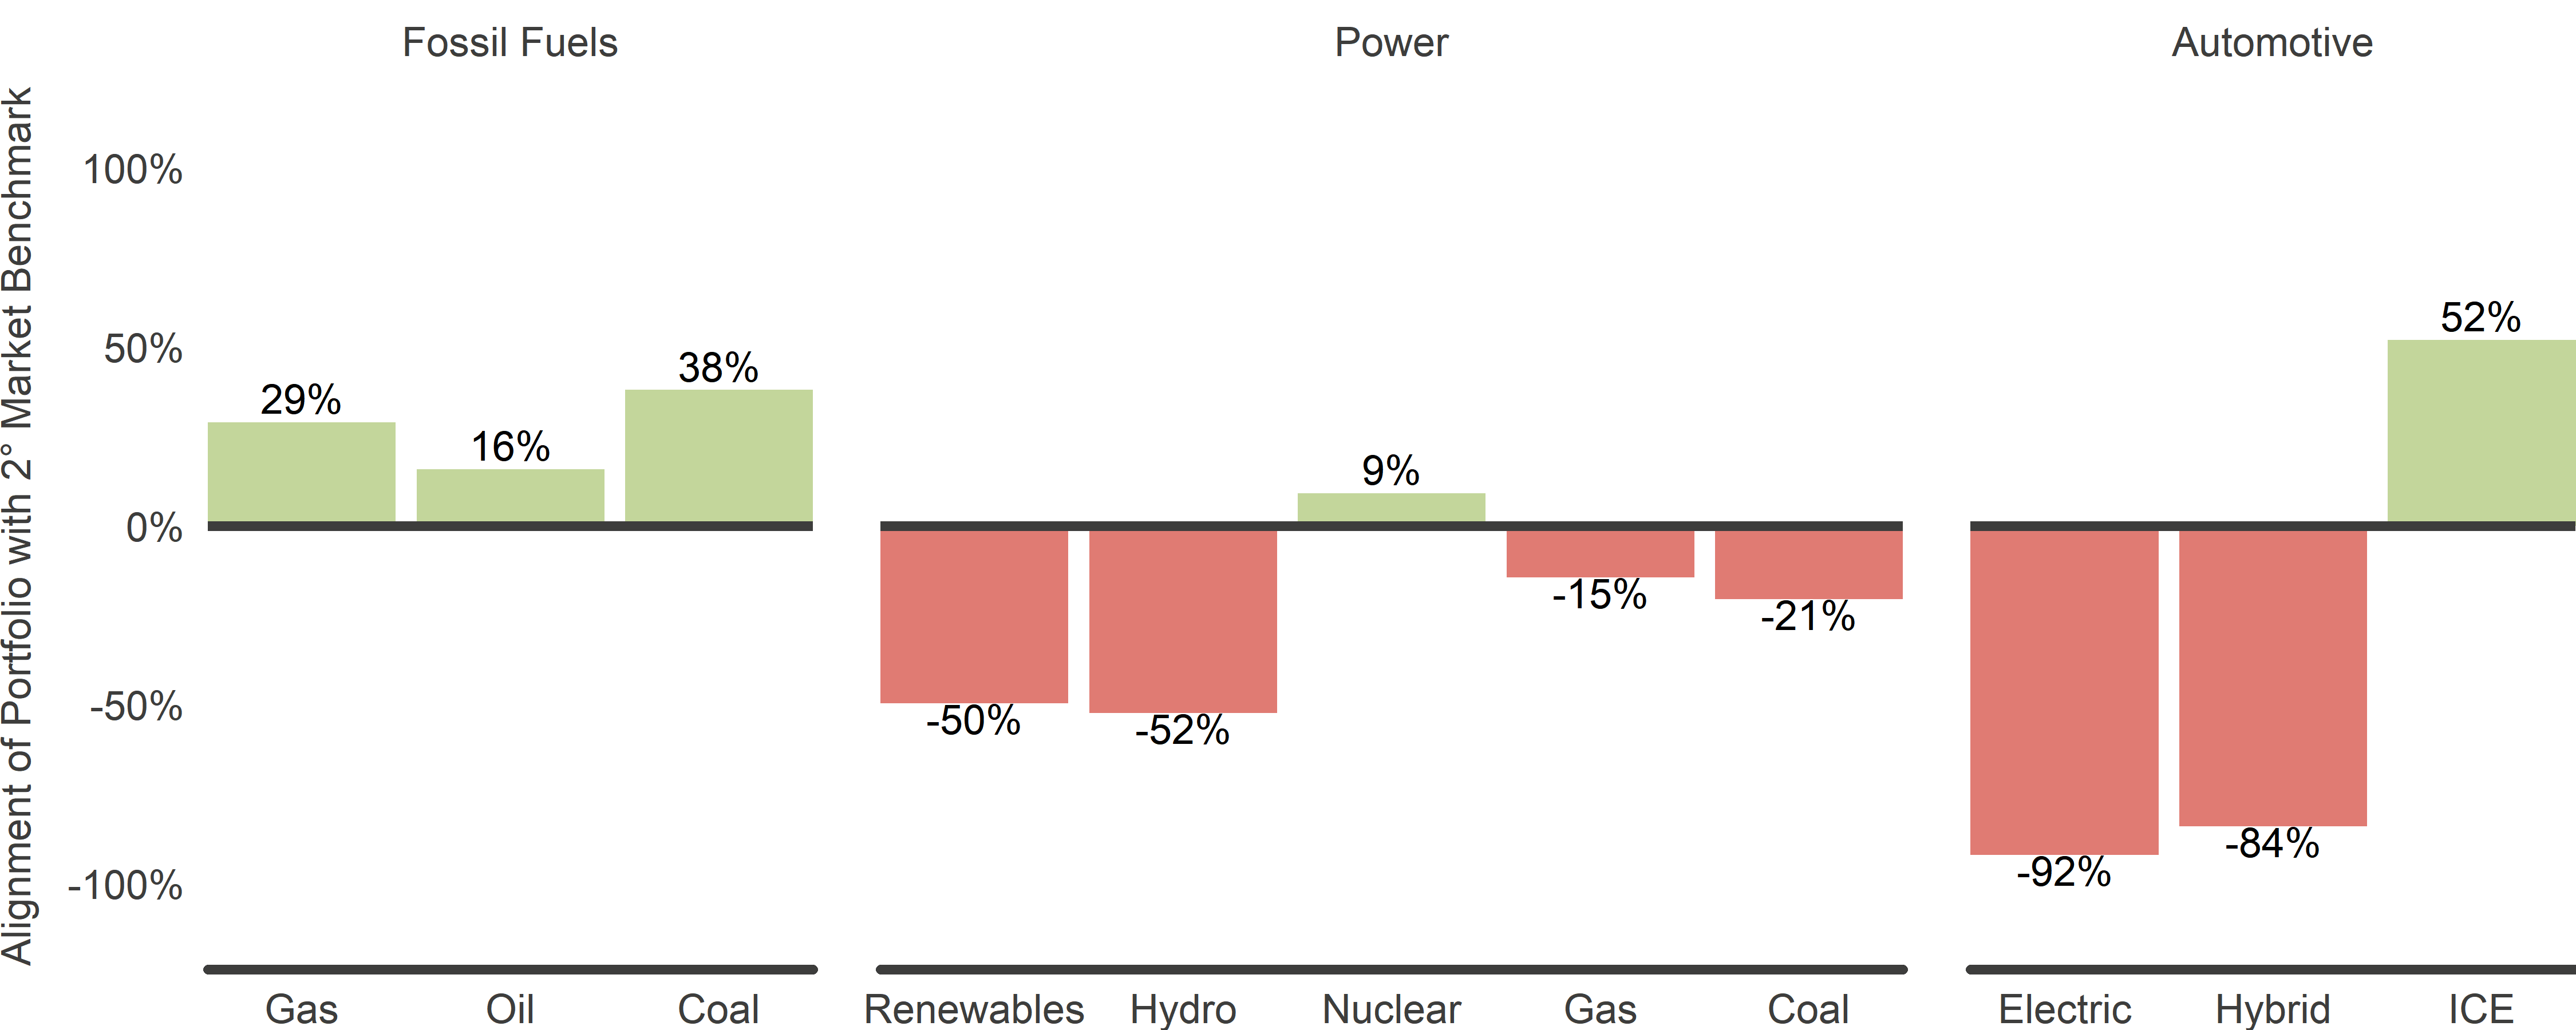
\includegraphics[trim = {0 0cm 0 0cm},width=1\linewidth]{Figures/Fig07} %CBSpecificE
	

		\textbf{Equity portfolio deviation from the benchmark in climate-relevant technologies in 2023} %EQSpecificS
		
		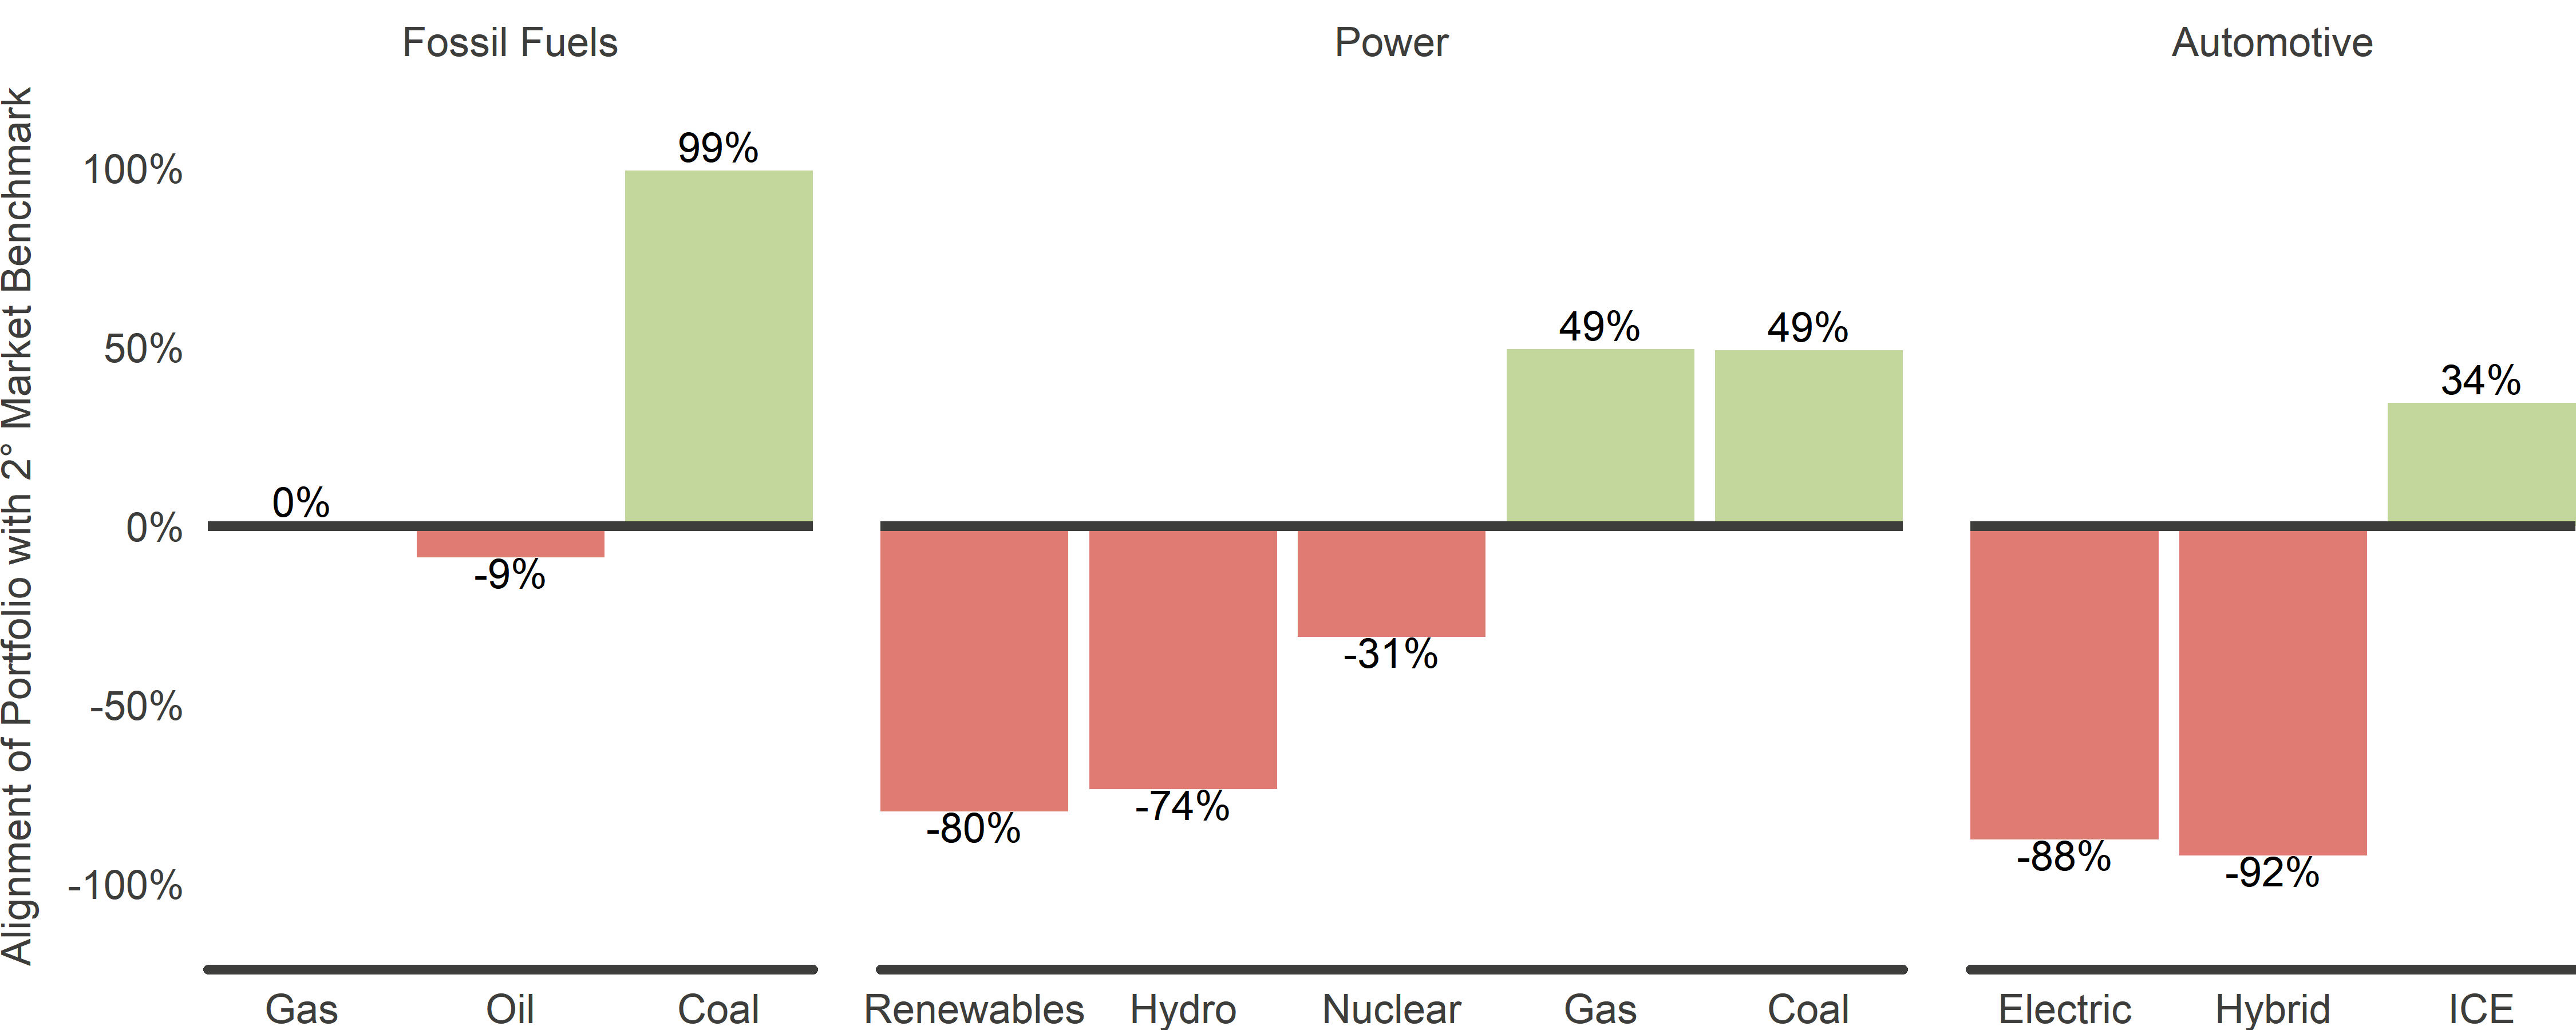
\includegraphics[trim = {0 0cm 0 0cm},width=1\linewidth]{Figures/Fig06}	%EQSpecificE	
		


	\newpage
\section*{} % 1st Section
\SectionHeading{SECTION 1:}{INTRODUCTION}
	

	\newpage
	\section*{} % Report Contents
	\HeaderSingle{REPORT CONTENTS}
	
	\begin{multicols}{2}
	
		\textbf{This report provides a scenario analysis of your equity and bond portfolios, following the recommendations of the G20's Task Force on Climate-Related Financial Disclosures (TCFD). It also addresses your 2° target alignment as agreed upon by the international community in the Paris Agreement. Specifically, it seeks to inform the reader about four issues.}
		
		\begin{enumerate}
			\item{\textbf{What is the current exposure of my portfolio to the 2°C scenario and transition risk? (Section 2)}
			}
			
			The first part of the report summarizes the exposures of the portfolio (in terms of \% of the portfolio) to business activities potentially affected by the transition to a low-carbon economy and by extension more broadly its exposure to transition risk. Specifically, it will quantify the percent of the portfolio that can be included in 2°C scenario analysis, the relative exposure to low-carbon and high-carbon fuels and technologies across the energy, power, and automobile sector, as well as the application of the Moody’s environmental risk assessment framework on the debt portfolio. The analysis will also benchmark the results compared to the peers included in this assessment and a market portfolio.
			
			\item{\textbf{Is my portfolio building or reducing risk in terms of being aligned / misaligned with a 2°C transition over the next 5 years? (Section 3)}
			}
			
			The second part of the report will quantify the extent to which the portfolio is building or reducing risk in terms of being aligned / misaligned with the 2°C scenario pathway over the next 5 years across key business activities. The analysis will focus on the fossil fuel related sectors in terms of energy (oil production, gas production), electric power (coal power, gas power, nuclear power, renewables power), and automobile (Internal combustion engine vehicles and electric vehicles). The analysis will currently planned production / investment trend in the portfolio with the production / investment that would be requried under the 2°C scenario. 
			
			\item{\textbf{What is my expected alignment in 5 five years? (Section 4)}
			}
			
			The third part of the report will quantify the extent to which your portfolio's currently planned production / investments until 2023 over- or under-weight high-carbon and low-carbon technologies, relative to a market portfolio in alignment with the 2° benchmark.
			
			\item{\textbf{What is driving the results? (Section 5)}}
			
			The final section will provide some more granular information on the companies behind the securities in your portfolio and the extent to which they are driving the results.
			
			You will also be able to find further background information on the scenarios and modelling at the end of the report.
			
			
		\end{enumerate}
				
	\end{multicols}

%	\vspace{1cm}
	\begin{tikzpicture}[remember picture, overlay]
		\node[anchor=north west,minimum width=.375cm,minimum height=6.5cm,fill=Yellow1] (ToC) at (-1.2,-.4){};
		\end{tikzpicture}	
	
	\begin{minipage}[t]{.5\linewidth}
		\textbf{Section 1: }Introduction\\
		
		\textbf{Section 2: }Current exposure to transition risk and 2°C scenario\\
		
		\textbf{Section 3: }5 Year Trend of transition risk and alignment with 2°C, 4°C, 6°C scenarios\\
		
		\textbf{Section 4: }Exposure in 5 years to transition risk and 2°C scenario \\
		
		\textbf{Section 5: }Company information\\
		
		\textbf{Section 6: }Capacity building on 2° transition scenarios and methodology\\
	\end{minipage}

	\PageFooterFirst
	\newpage
\section*{} % 2nd Section
\SectionHeading{SECTION 2:}{THE CURRENT EXPOSURE}
		
	\newpage
	\section*{} % 2° SCENARIO - CURRENT EXPOSURE 2018
	\HeaderSingle{2° SCENARIO - CURRENT EXPOSURE 2018}
	
		\begin{multicols}{2}
		
			
			\textbf{This page provides information on the exposure of the portfolio to business activities covered in 2°C scenarios. }
			
			These business activities account for roughly 70-90\% of GHG emissions in the typical investor portfolio. The figure on the right shows the percent of the portfolio (by asset class) exposed to the fossil fuels, power, and automotive sectors. The figures below show the weight of each technology/fuel within each sector, by asset class. The graphs below highlight the relative weight of high-carbon and low-carbon technologies within each sector.  For context, the results for a portfolio of peer companies and the relevant stock or bond market is also included in this analysis.
			
			
			\textbf{Share of the portfolio exposed to business activities covered by the International Energy Agency 2°C scenario}
			
			\vspace{-.2cm}
			\center{\adjincludegraphics[width = .8\linewidth,trim={0cm 0.2cm 0cm 0cm},clip]{Figures/Fig02}	}
			\vspace{-1.2cm}
			\newline
				
			
		\end{multicols}
		
		\vspace{.3cm}
		
			\textbf{Technology breakdown of the sectors analyzed in your bond portfolio} %CBSpecificS
			
			\vspace{-0.2cm}
			
			\adjincludegraphics[width = 1\linewidth,trim={0cm 0cm 0cm 0cm},clip]{Figures/Fig10}	
			%CBSpecificE


			\textbf{Technology breakdown of the sectors analyzed in your equity portfolio} %EQSpecificS

			\vspace{-0.2cm}
			
			\adjincludegraphics[width = 1\linewidth,trim={0cm 0cm 0cm 0cm},clip]{Figures/Fig09}
			
			%EQSpecificE
		
	\PageFooterSecond
	\newpage	
%	\section*{} % 2°C SCENARIO CURRENT EXPOSURE – COMPARISION TO PEERS
%	\HeaderDouble{2°C SCENARIO CURRENT EXPOSURE}{COMPARISION TO PEERS}	
%	
%	
%		\begin{multicols}{2}
%			\textbf{This page provides information on the comparison of the exposure of the portfolio to transition risk among investors.}
%			
%			It takes the information from the previous page and contextualizes it relative to the other investors compared in this assessment. More specifically it compares the distribution of fossil fuel exposure within all portfolios. The results show that for bond portfolios no portfolio has an exposure to fossil fuels greater than 10\% For equity portfolios, the distribution is greater ranging from 0\% exposure to 100\% exposure.
%			
%		\end{multicols}
%
%		
%	
%		
%		\textbf{Distribution of exposure to Fossil fuels within all bond portfolios} %CBSpecificS
%		
%		\adjincludegraphics[width = 1\linewidth,trim={0cm 0cm 0cm 0cm},clip]{Figures/Fig12}	%CBSpecificE
%	
%	
%	
%		\textbf{Distribution of exposure to Fossil fuels within all equity portfolios} %EQSpecificS
%	
%		\adjincludegraphics[width = 1\linewidth,trim={0cm 0cm 0cm 0cm},clip]{Figures/Fig11} %EQSpecificE	 
%		
%		
%	\PageFooterSecond
%	\newpage
%	\section*{} % ENVIRONMENTAL RISK CURRENT EXPOSURE –BONDS %CBSpecificS
%	\HeaderSingle{ENVIRONMENTAL RISK CURRENT EXPOSURE - BONDS}	
%
%		\begin{multicols}{2}
%					\textbf{For the bonds portfolios, Moody’s has developed an environmental risk sector classification that goes beyond climate to a broader suite of environmental risks.} 
%			
%			The classification – developed in 2015 / 2016 – has been previously applied by a range of insurance companies and supervisors to identify risk exposures. Moody’s creates a risk level for each bond based on the sector in which they operate.  These ratings are based on sectoral breakdown. 
%			
%			\textbf{The following four risk levels are represented in the classification:  }
%		\end{multicols}
%
%		
%		\begin{center}
%			{\setlength{\tabcolsep}{10pt} % Default value: 6pt
%				\renewcommand{\arraystretch}{1.5} % Default value: 1
%				\begin{tabular}{ p{.2\linewidth}| p{.7\linewidth} }
%					\hline
%					\textbf{Risk Level} & \textbf{Sector}  \\ 
%					\hline
%					\cellcolor{ColRed} Immediate Elevated & Independent Power Producers, Coal and Consumable Fuels \\ 
%					\hline
%					\cellcolor{ColOrange} Emerging Elevated & Steel, Aluminum, Oil and Gas E\&P, Construction Materials, Diversified Metals and Mining, Auto Manufacturers \\ 
%					\hline
%					\cellcolor{ColYellow} Emerging Moderate & Regulated Utilities, Airlines, Integrated Oil and Gas, Paper, Oil and Gas services, Auto Parts, Gas Utilities \\ 
%					\hline
%					\cellcolor{ColGreen} Low & Marine, Diversified Chemicals, Industrial Gases, Marine Ports  \\ 
%					\hline
%				\end{tabular}
%			}
%		\end{center}
%		
%		\begin{multicols}{2}
%			\textbf{The following chart presents the percentage of your portfolio by AUM that is rated as Immediate Elevated, Emerging Elevated or Emerging Moderate.} 
%			
%			While there is some variation, almost all investors, have some exposure to sectors of elevated risk. While this is primarily only in emerging elevated sectors, it gives an indication that the invested debt market is quite exposed to risk. 
%			
%			The portfolio is above the average in terms of environmental risk exposure, the average being 11\%. Crucially, the assessment provided here does not build on the 	type of granularity described earlier in terms of high-carbon and low-carbon exposures, but remains at sector level. It is thus by design more imprecise than alternative approaches.
%		\end{multicols}	
%		
%		
%		\textbf{The environmental risk exposure of your portfolio relative to its peers}
%		
%		\begin{centering}
%					
%			\adjincludegraphics[width = 1\linewidth,trim={0cm 0cm 0cm 0cm},clip]{Figures/Fig13}
%		\end{centering}
%		
%\PageFooterSecond
%\newpage	%CBSpecificE
\section*{} % 3rd Section
\SectionHeadingDouble{SECTION 3:}{TRAJECTORY OF THE PORTFOLIO}{RELATIVE TO A 2°C SCENARIO}
	
	
	\newpage	
	\section*{} % TRAJECTORY – BONDS – POWER  %CBSpecificS
	\HeaderDouble{5 YEAR TREND - BONDS}{POWER}		

		\begin{multicols}{2}
			\textbf{The alignment graphs below show the alignment of selected power technologies in your bond portfolio relative to the IEA scenarios for 2°C, 4°C and 6°C temperature change, the global bond universe and the average of the comparison group.} 
			
			These charts present the trajectory of buildout in the power sector for the companies with production within your bond portfolio. This has been normalized to the 2°C benchmark, so the plotted lines show the difference to a 2°C scenario outcome. This is overlayed over the different IEA scenarios for these technologies, represented by the shaded background. This shows how the buildout of capacity allocated to your portfolio is aligned to the scenarios.  The forward-looking estimates for your portfolio are based on asset-level data analysis by sector and technology provided by GlobalData for the power and fossil fuel sector, and WardsAuto / AutoForecastSolutions for the automobile sector. Further background information on the data sources can be found in Section 5. 
			
		\end{multicols}
		
		\vspace{-.4cm}	
		
		\begin{minipage}[t]{.49\linewidth}
			\textbf{Trajectory of Coal Power Capacity }
		
			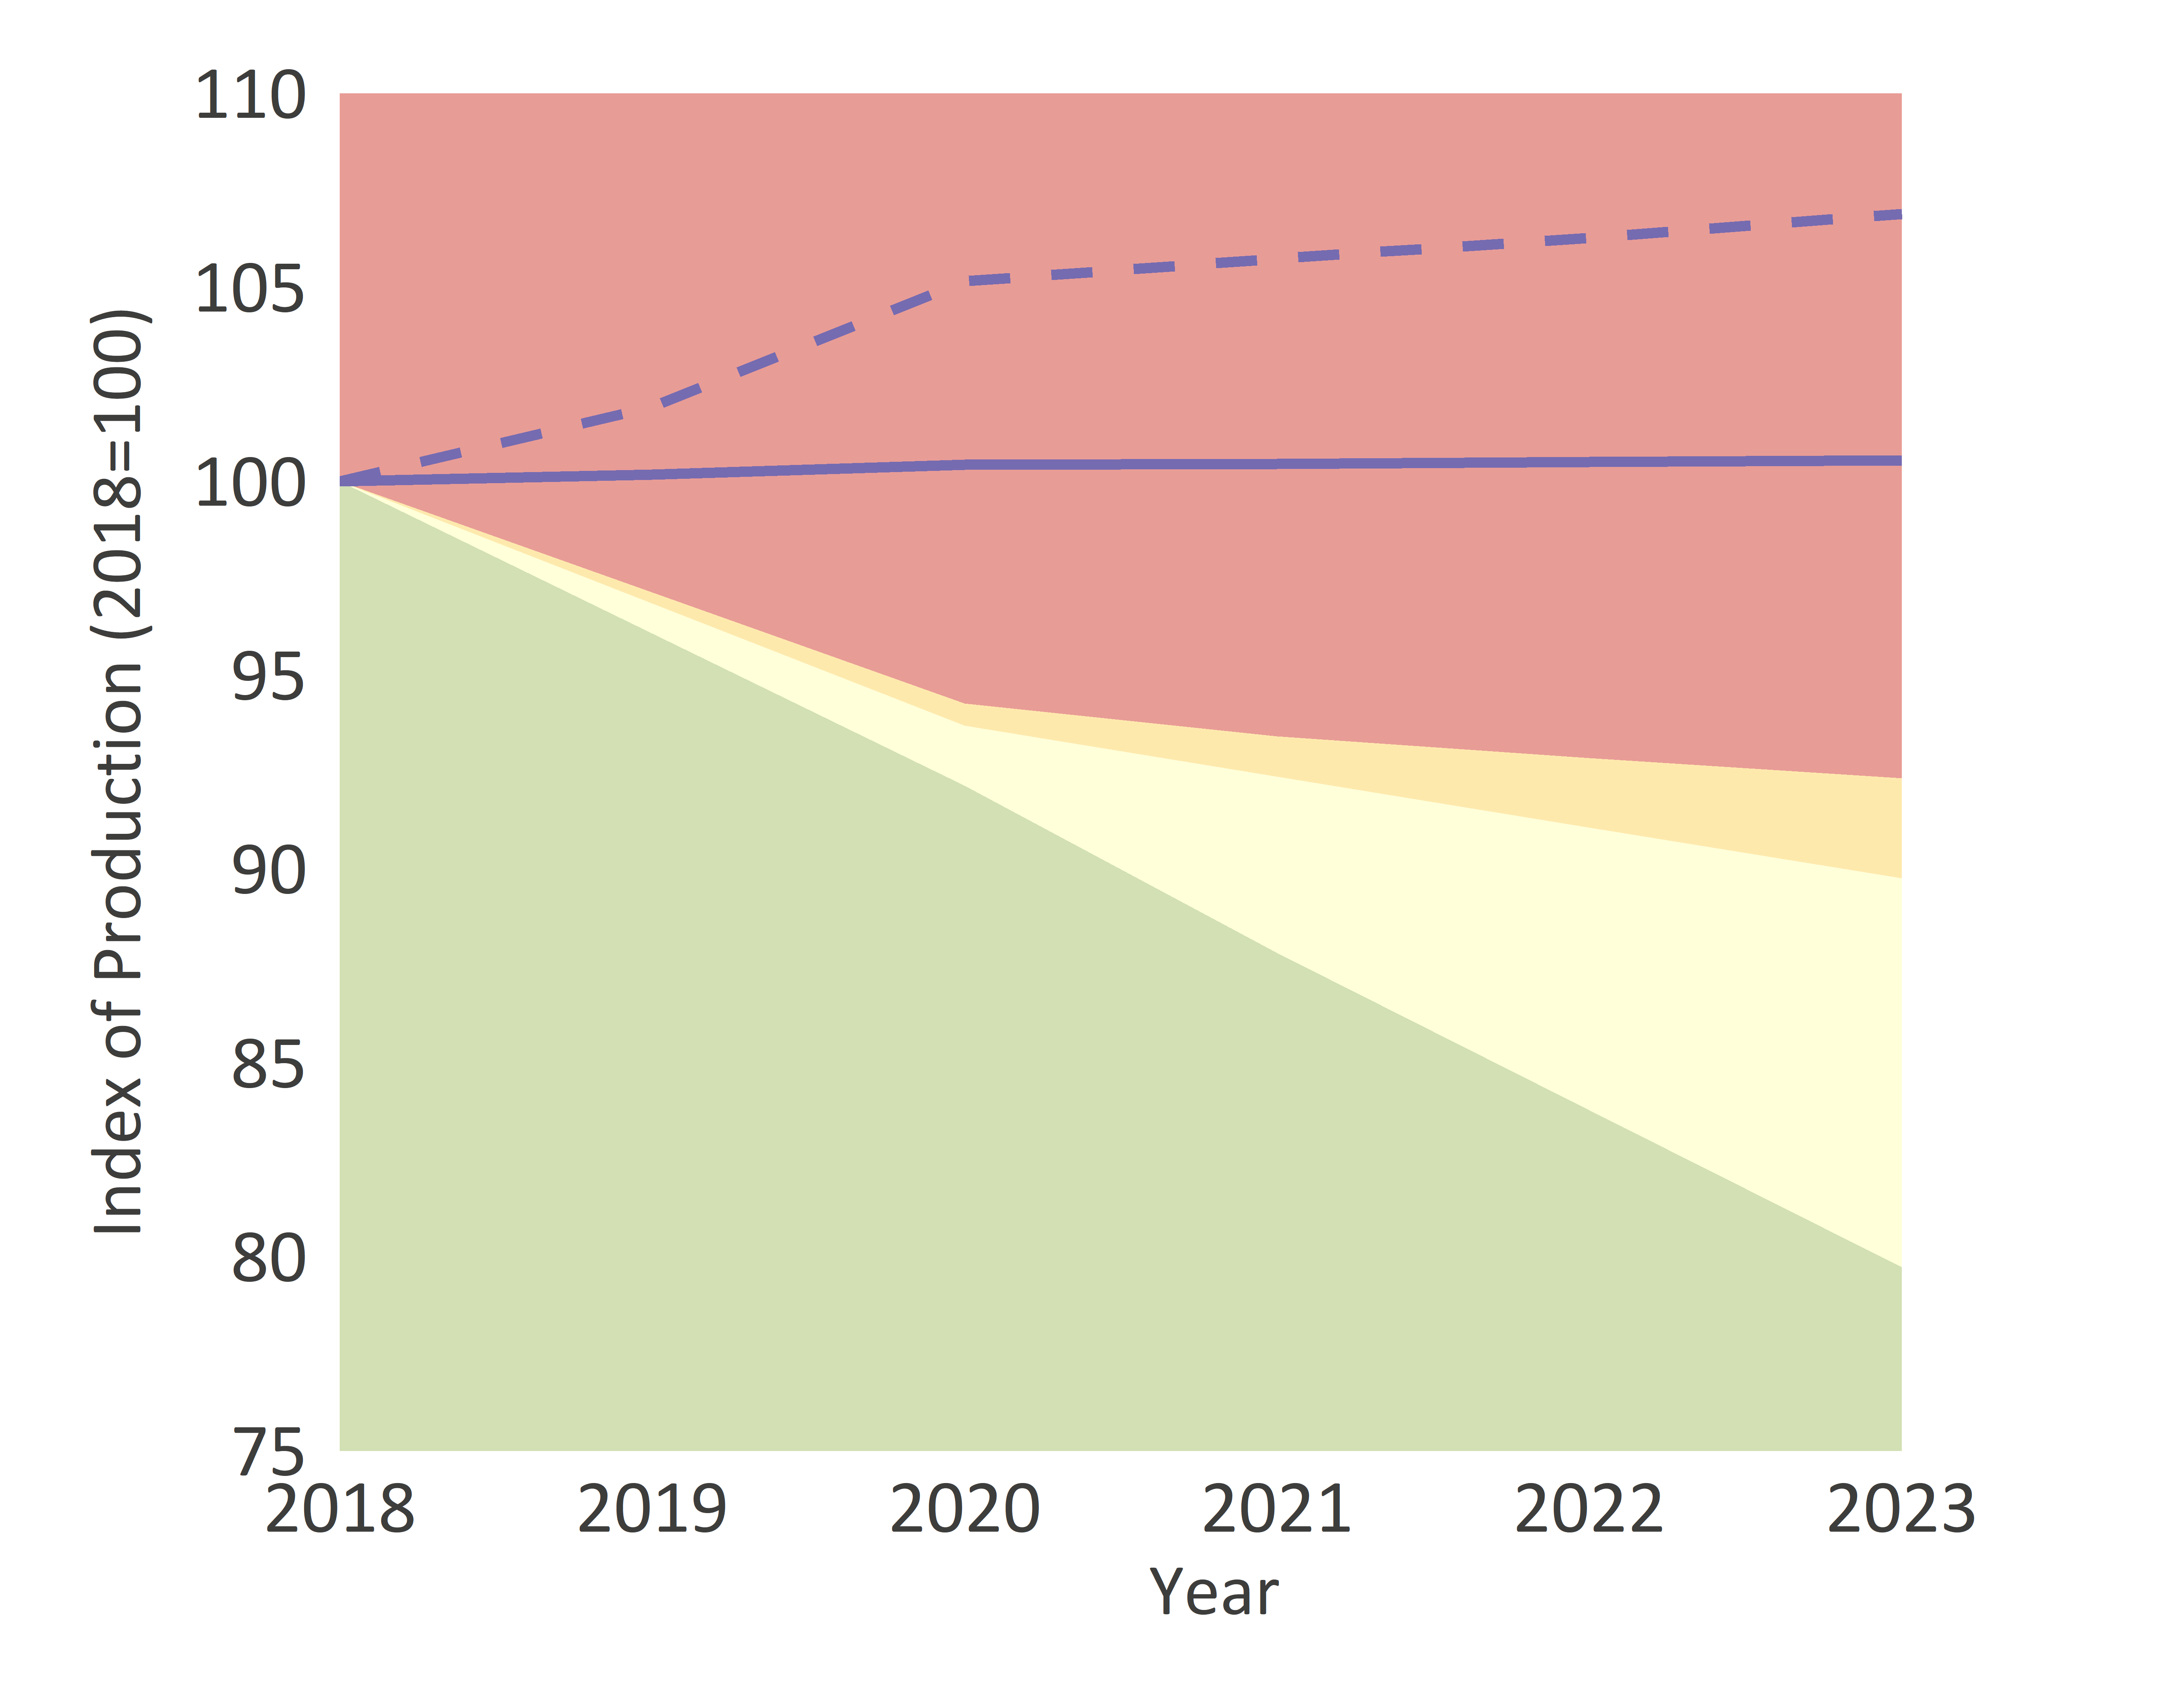
\includegraphics[trim = {0 0cm 0 0},width=1\linewidth]{Figures/Fig14}
			
			\textbf{Trajectory of Renewable Power Capacity }

			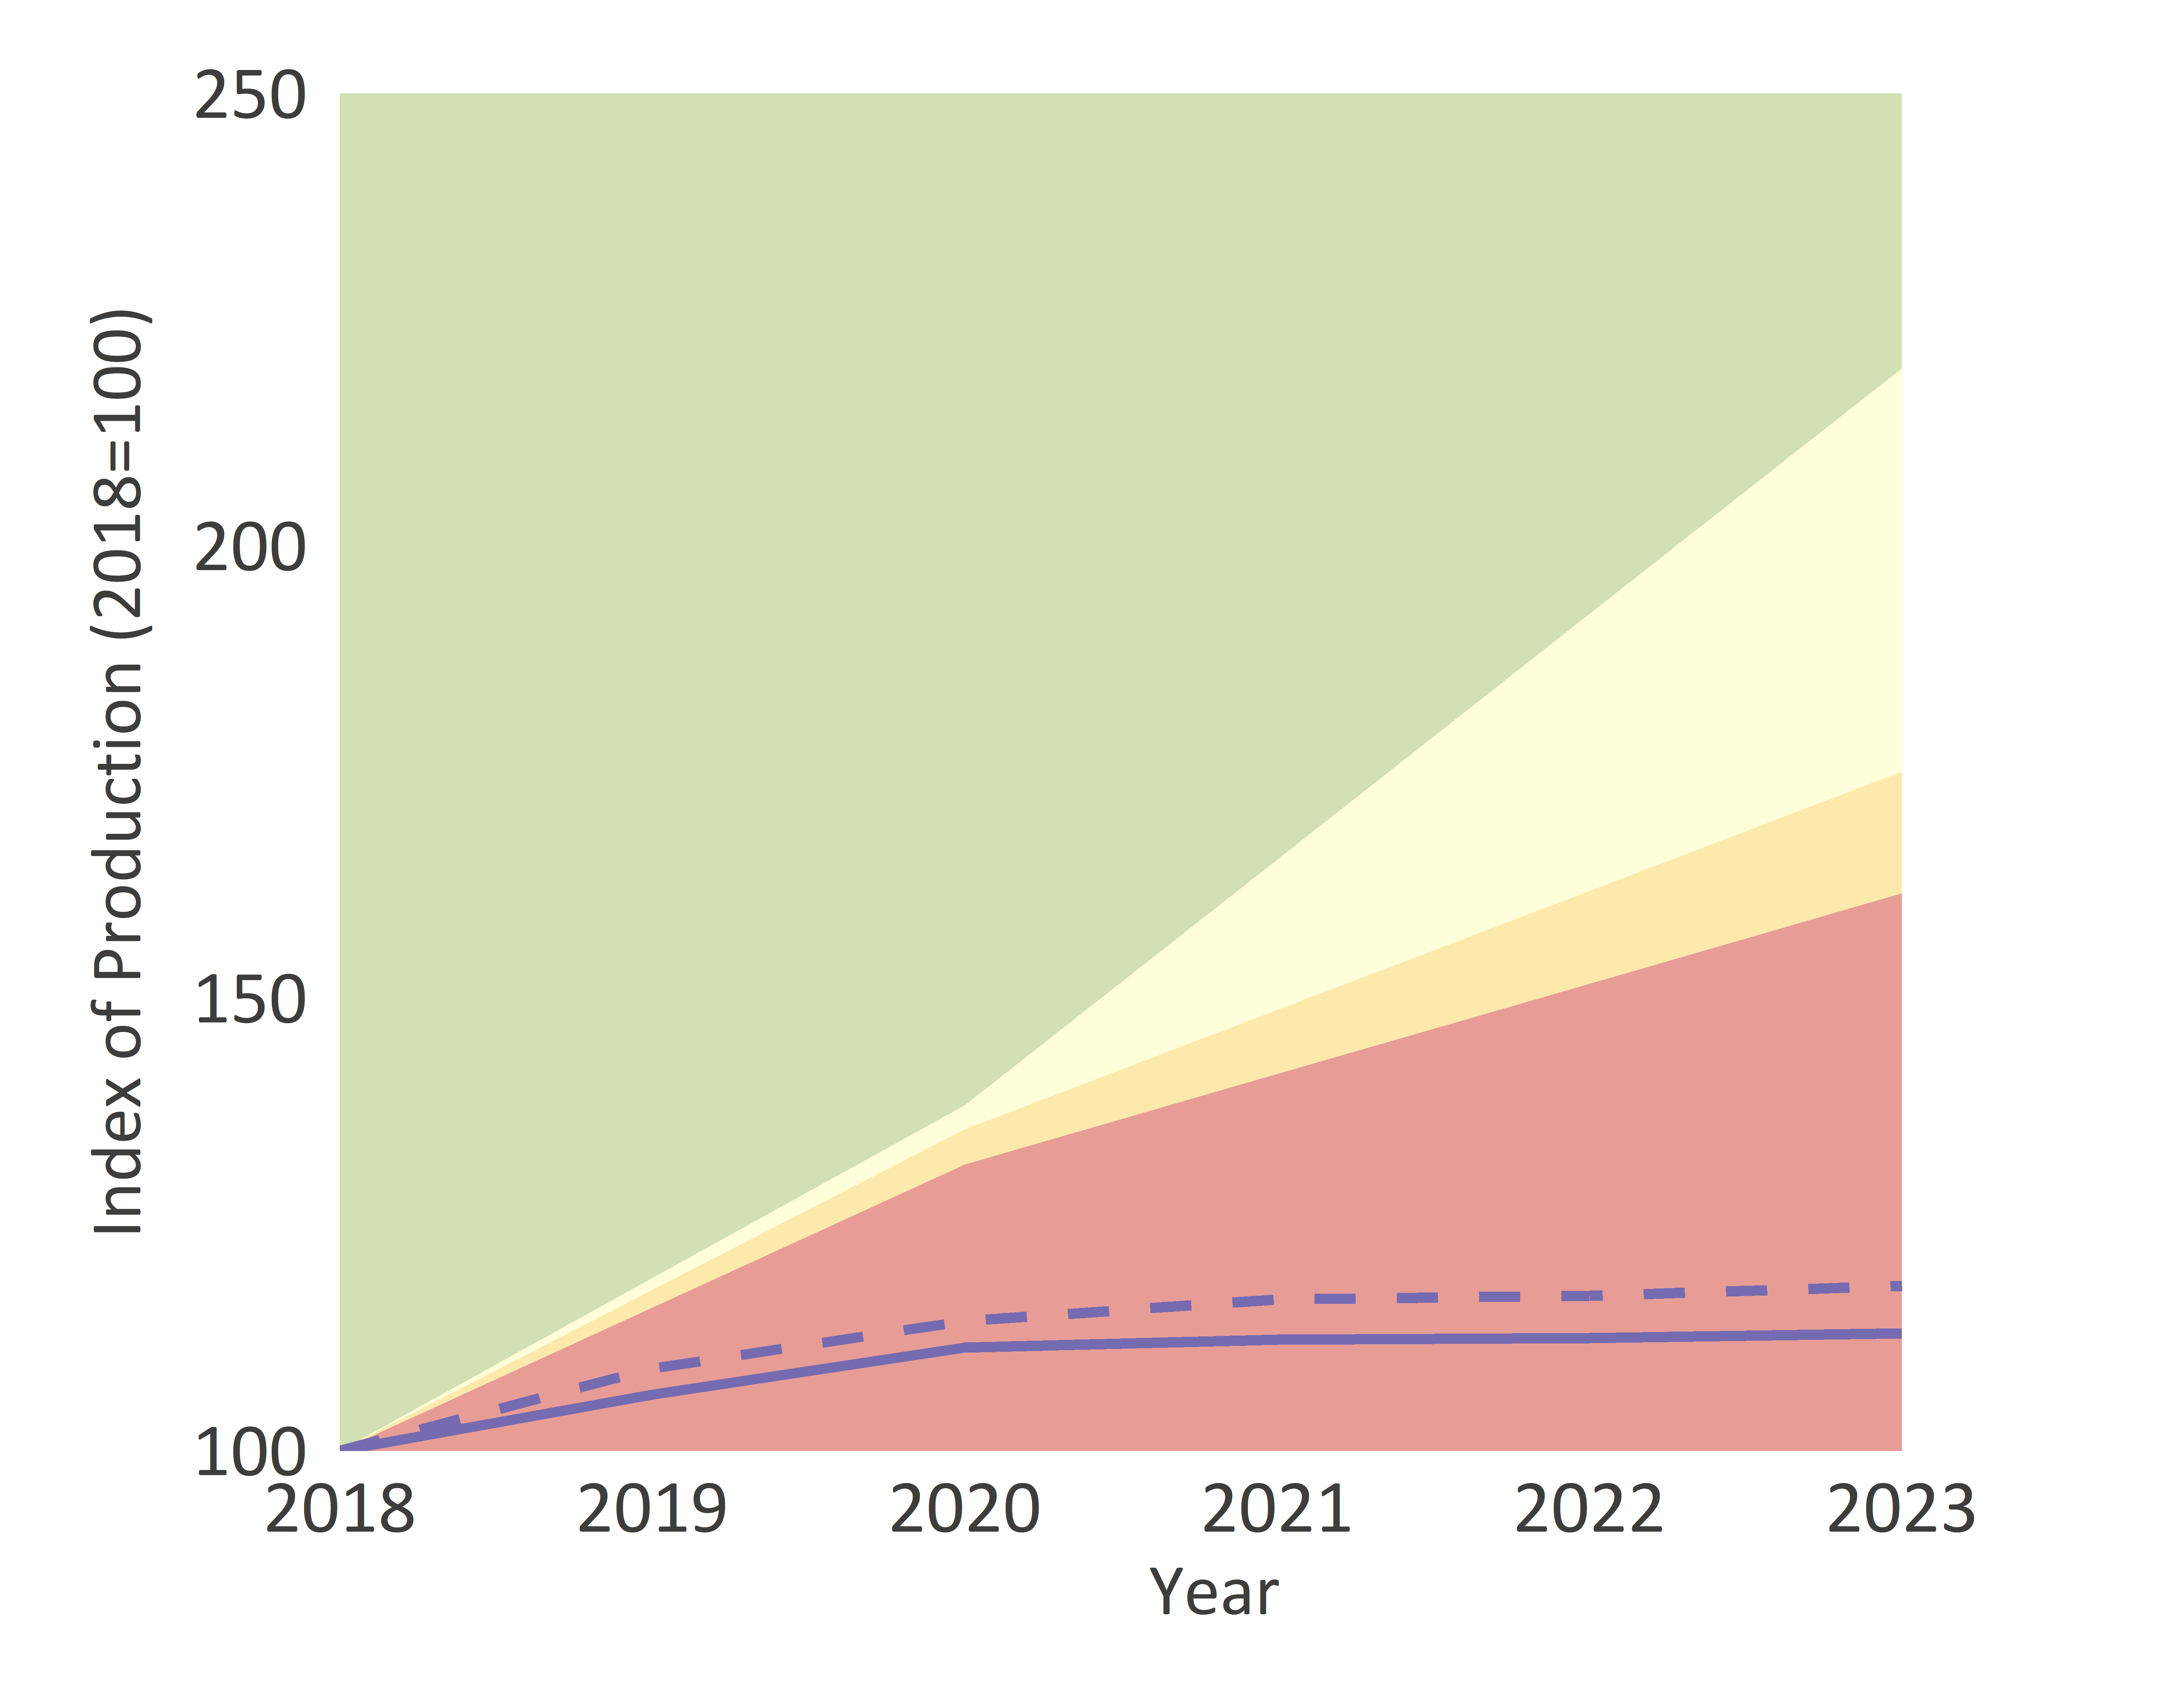
\includegraphics[trim = {0 0cm 0 0},width=.99\linewidth]{Figures/Fig15}
		\end{minipage}	
		\hspace{.02\linewidth}
		\begin{minipage}[t]{.49\textwidth}
			\textbf{Trajectory of Gas Power Capacity }
			
			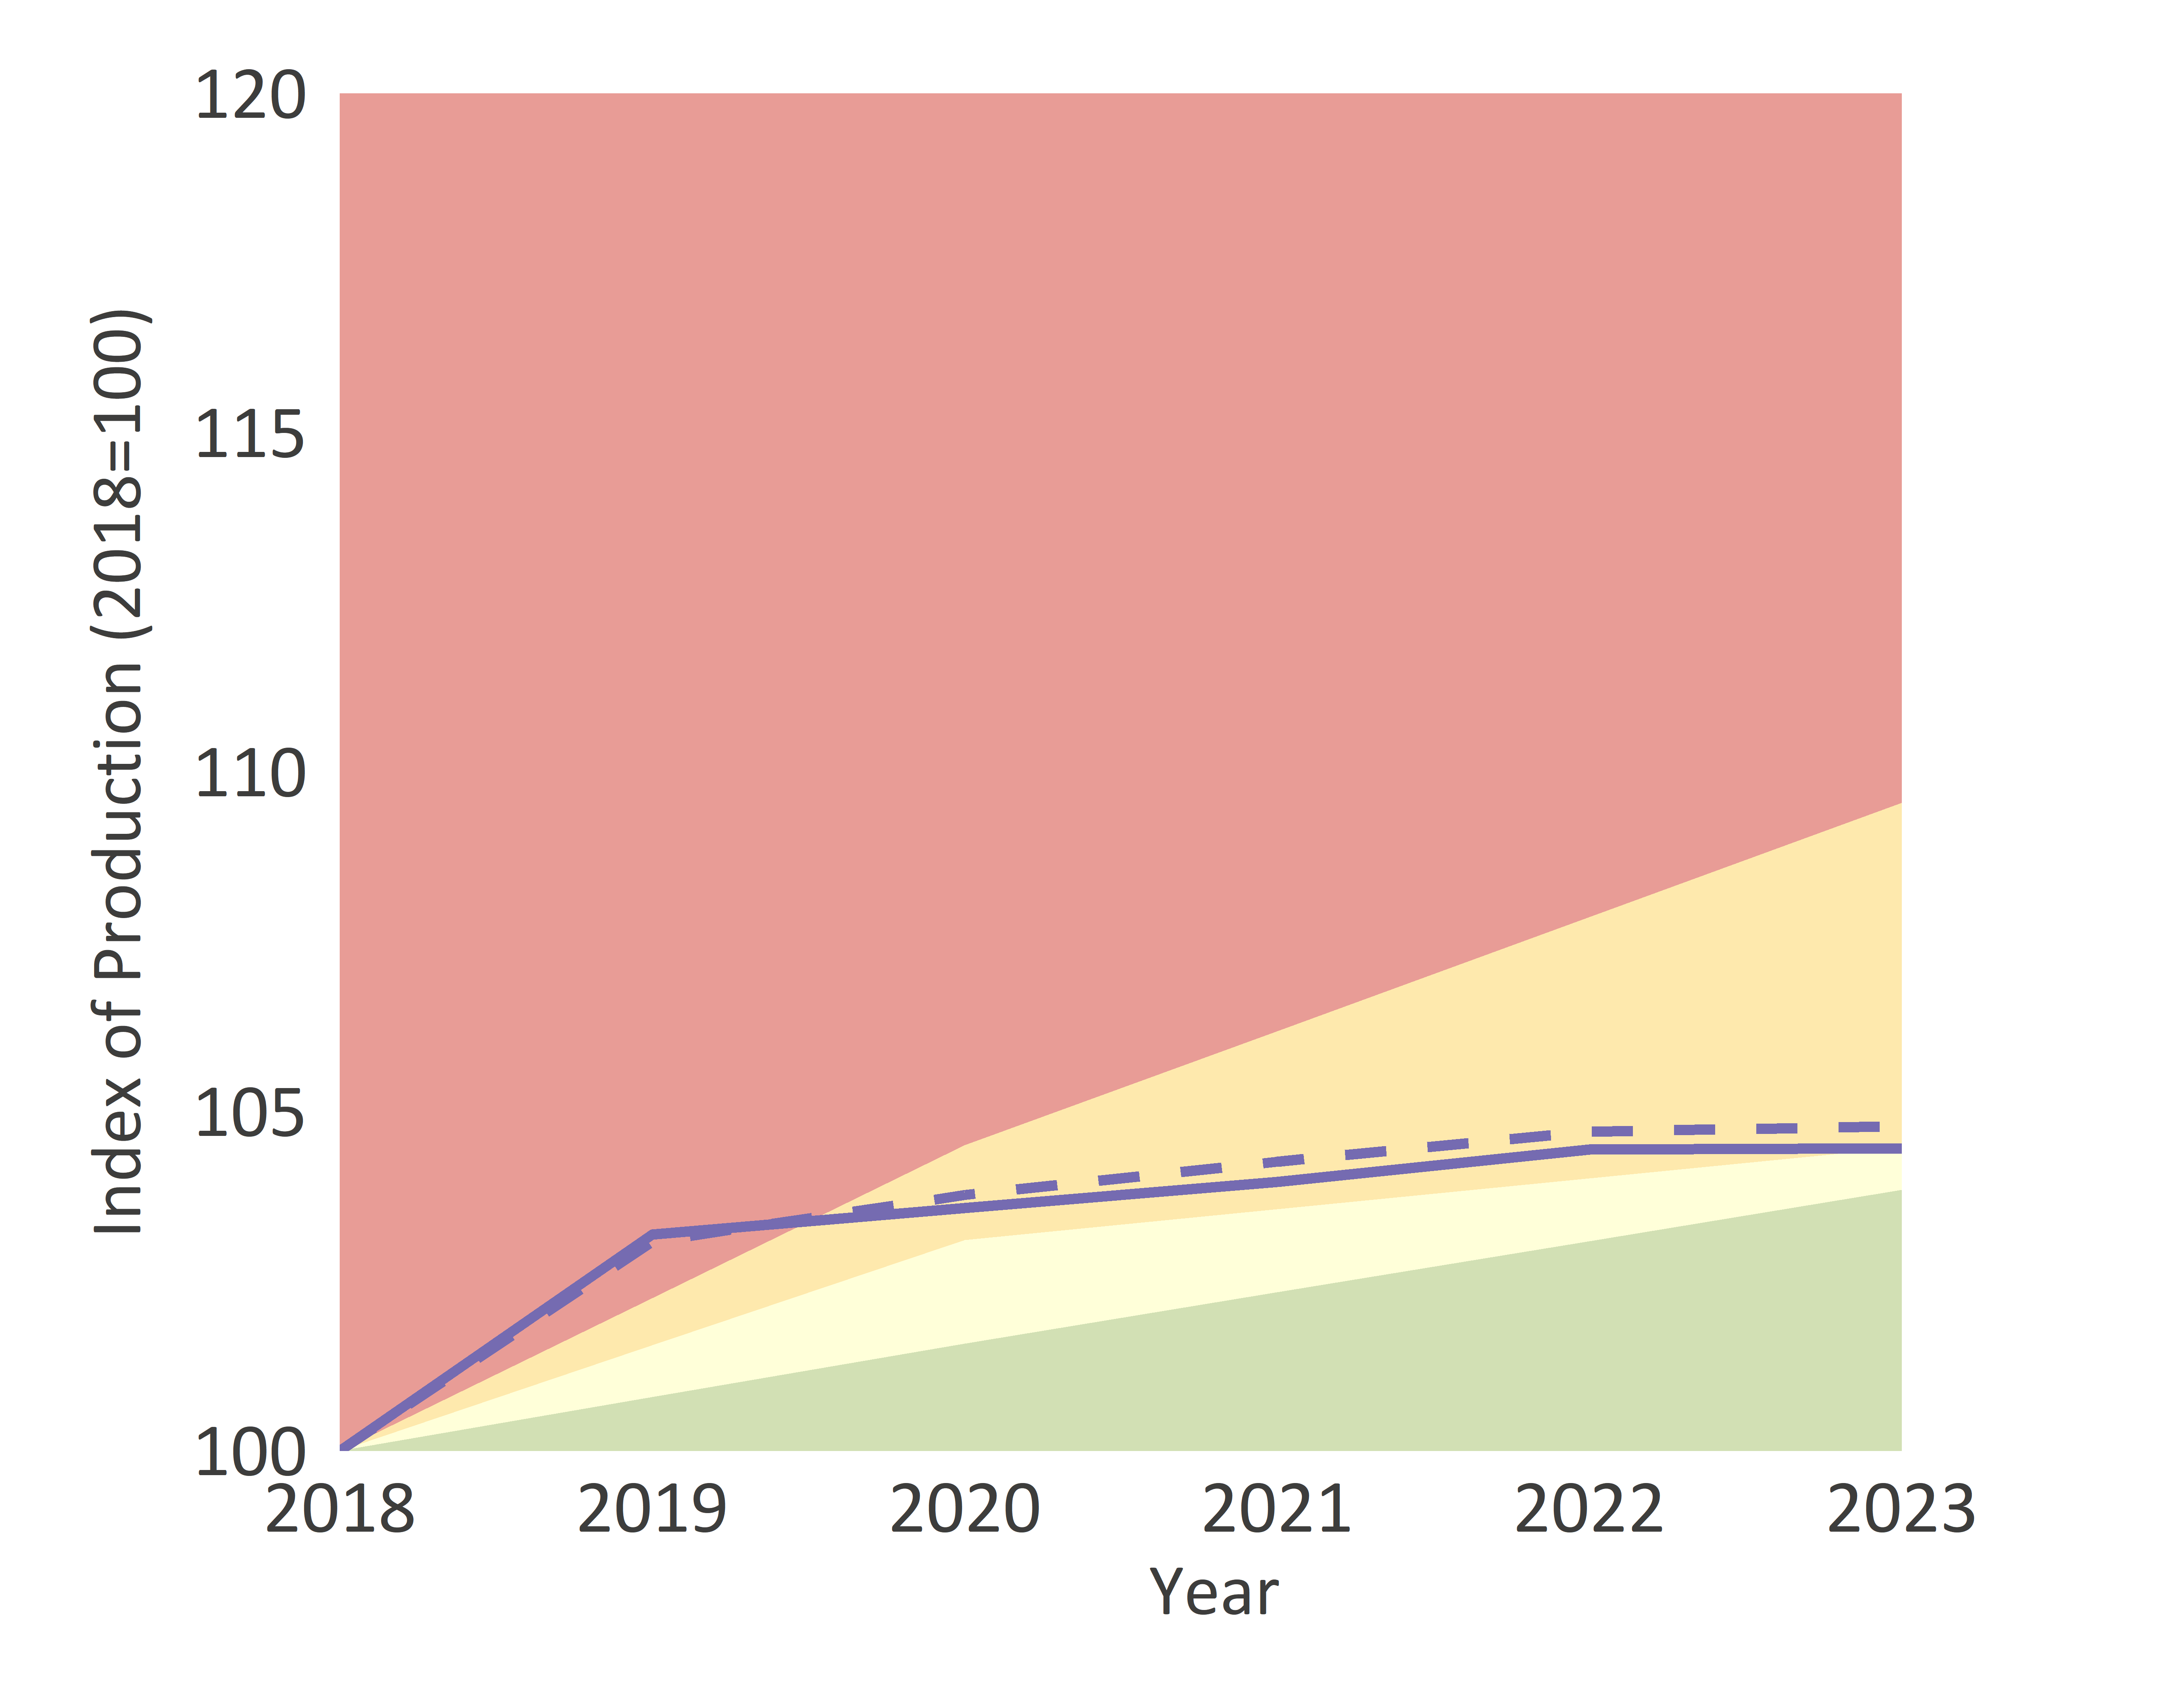
\includegraphics[trim = {0 0cm 0 0},width=1\linewidth]{Figures/Fig16}
		
			\textbf{Trajectory of Nuclear Power Capacity }
			
			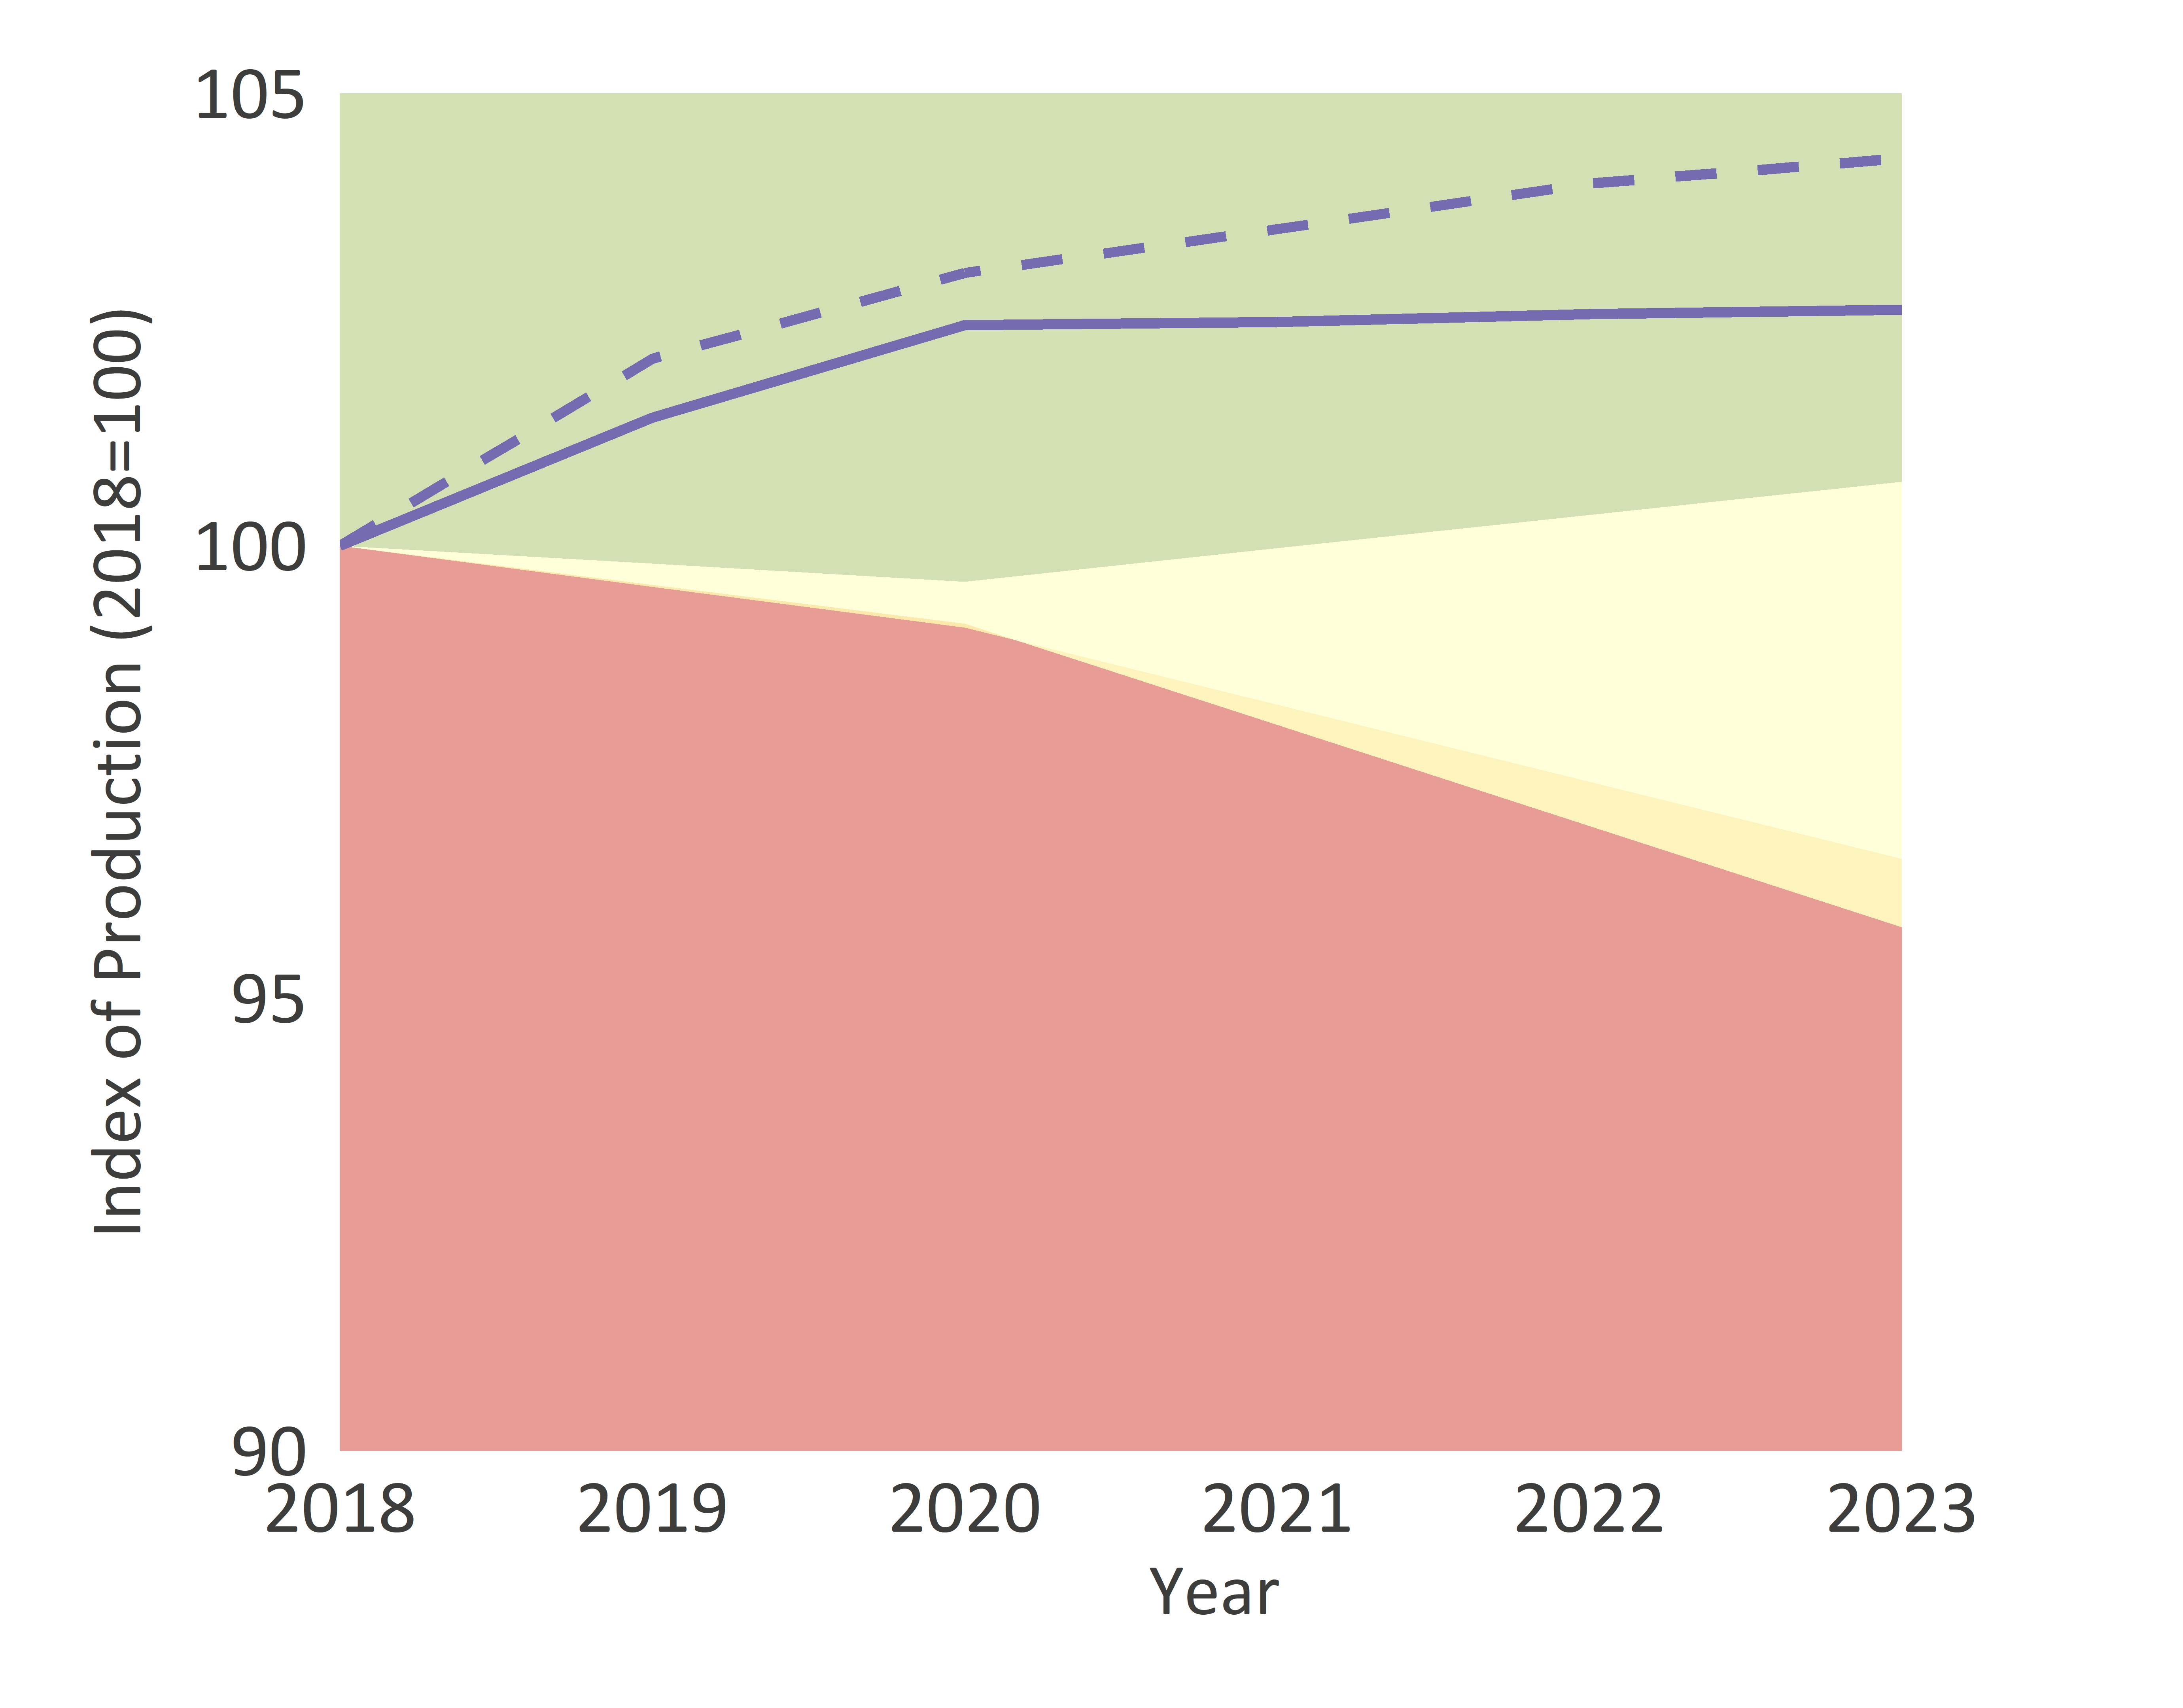
\includegraphics[trim = {0 0cm 0 0},width=1\linewidth]{Figures/Fig17}
	
		\end{minipage}
	
		\vspace{-0.4cm}
		\begin{center}
			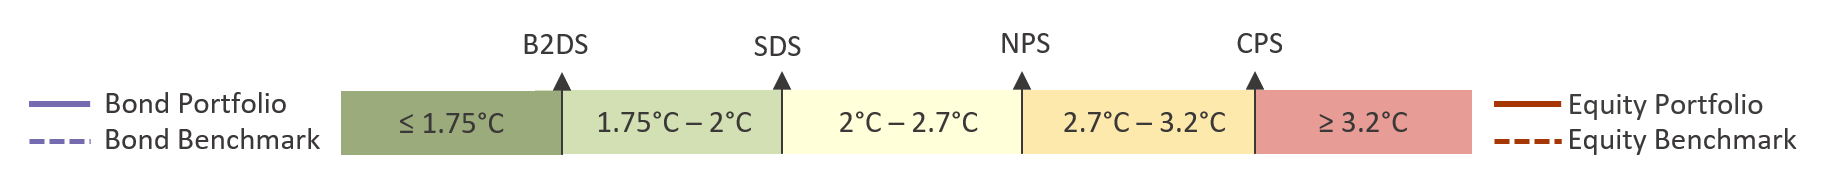
\includegraphics[trim = {0 0cm 0 0},width=.8\linewidth]{ReportGraphics/246Legend.png}
		\end{center}
		
		
	\PageFooterThird
	\newpage 
	\section*{} % TRAJECTORY – EQUITY – FOSSIL FUELS AND AUTOMOTIVE 
	\HeaderDouble{5 YEAR TREND - BONDS}{FOSSIL FUELS AND AUTOMOTIVE}	
		
		\begin{multicols}{2}
		\textbf{The alignment graphs below show the alignment of selected fossil fuels and automobile technologies in your bond portfolio relative to the IEA scenarios for 2°C, 4°C and 6°C temperature change, the global bond universe and the average of the comparison group. } 

		The page brings together data on the upstream supply of fossil fuels and the largest downstream user of oil, namely the automotive sector. It highlights the extent to which within a portfolio the strategies across sectors may be more or less consistent, relative to a 2°C scenario.
		
		\end{multicols}		
		
		\begin{center}
			\textbf{Fossil Fuel Sector}
		\end{center}
		
		\begin{minipage}[t]{.49\linewidth}
			\textbf{Trajectory of Oil Production }
		
			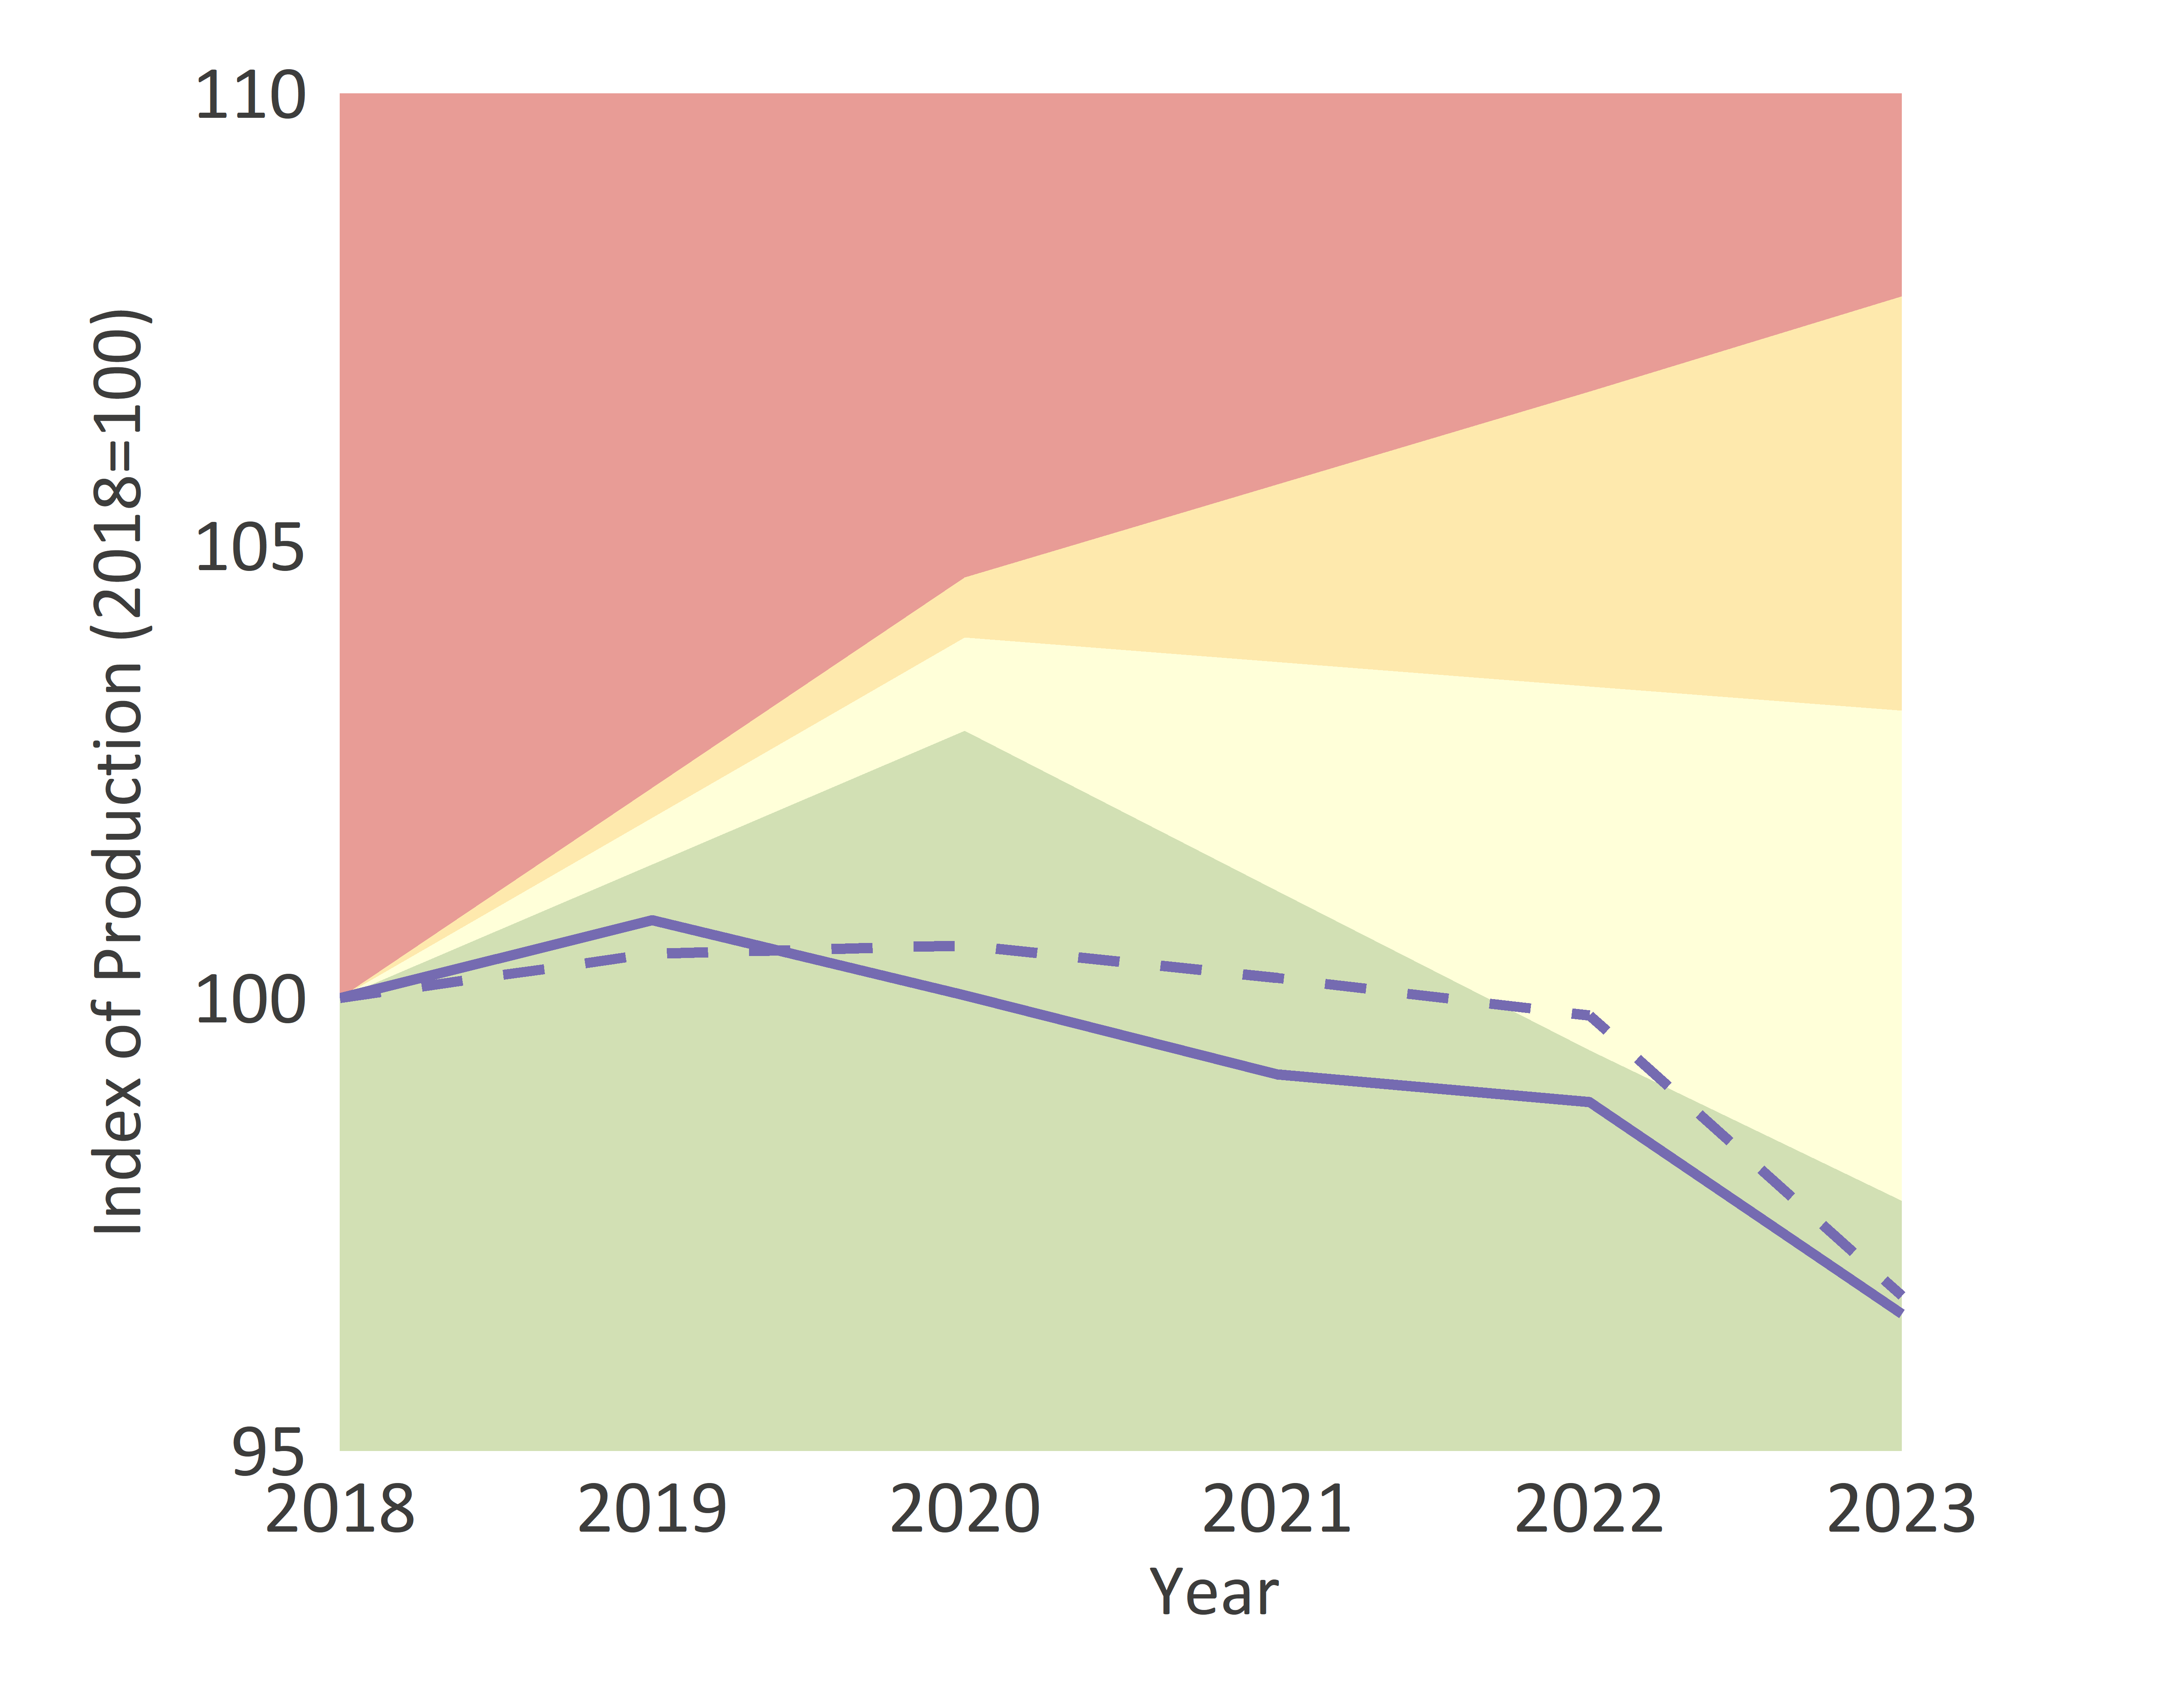
\includegraphics[trim = {0 0cm 0 0},width=1\linewidth]{Figures/Fig18}
			
		\end{minipage}	
		\hspace{.02\linewidth}
		\begin{minipage}[t]{.49\textwidth}
			\textbf{Trajectory of Gas Production }

			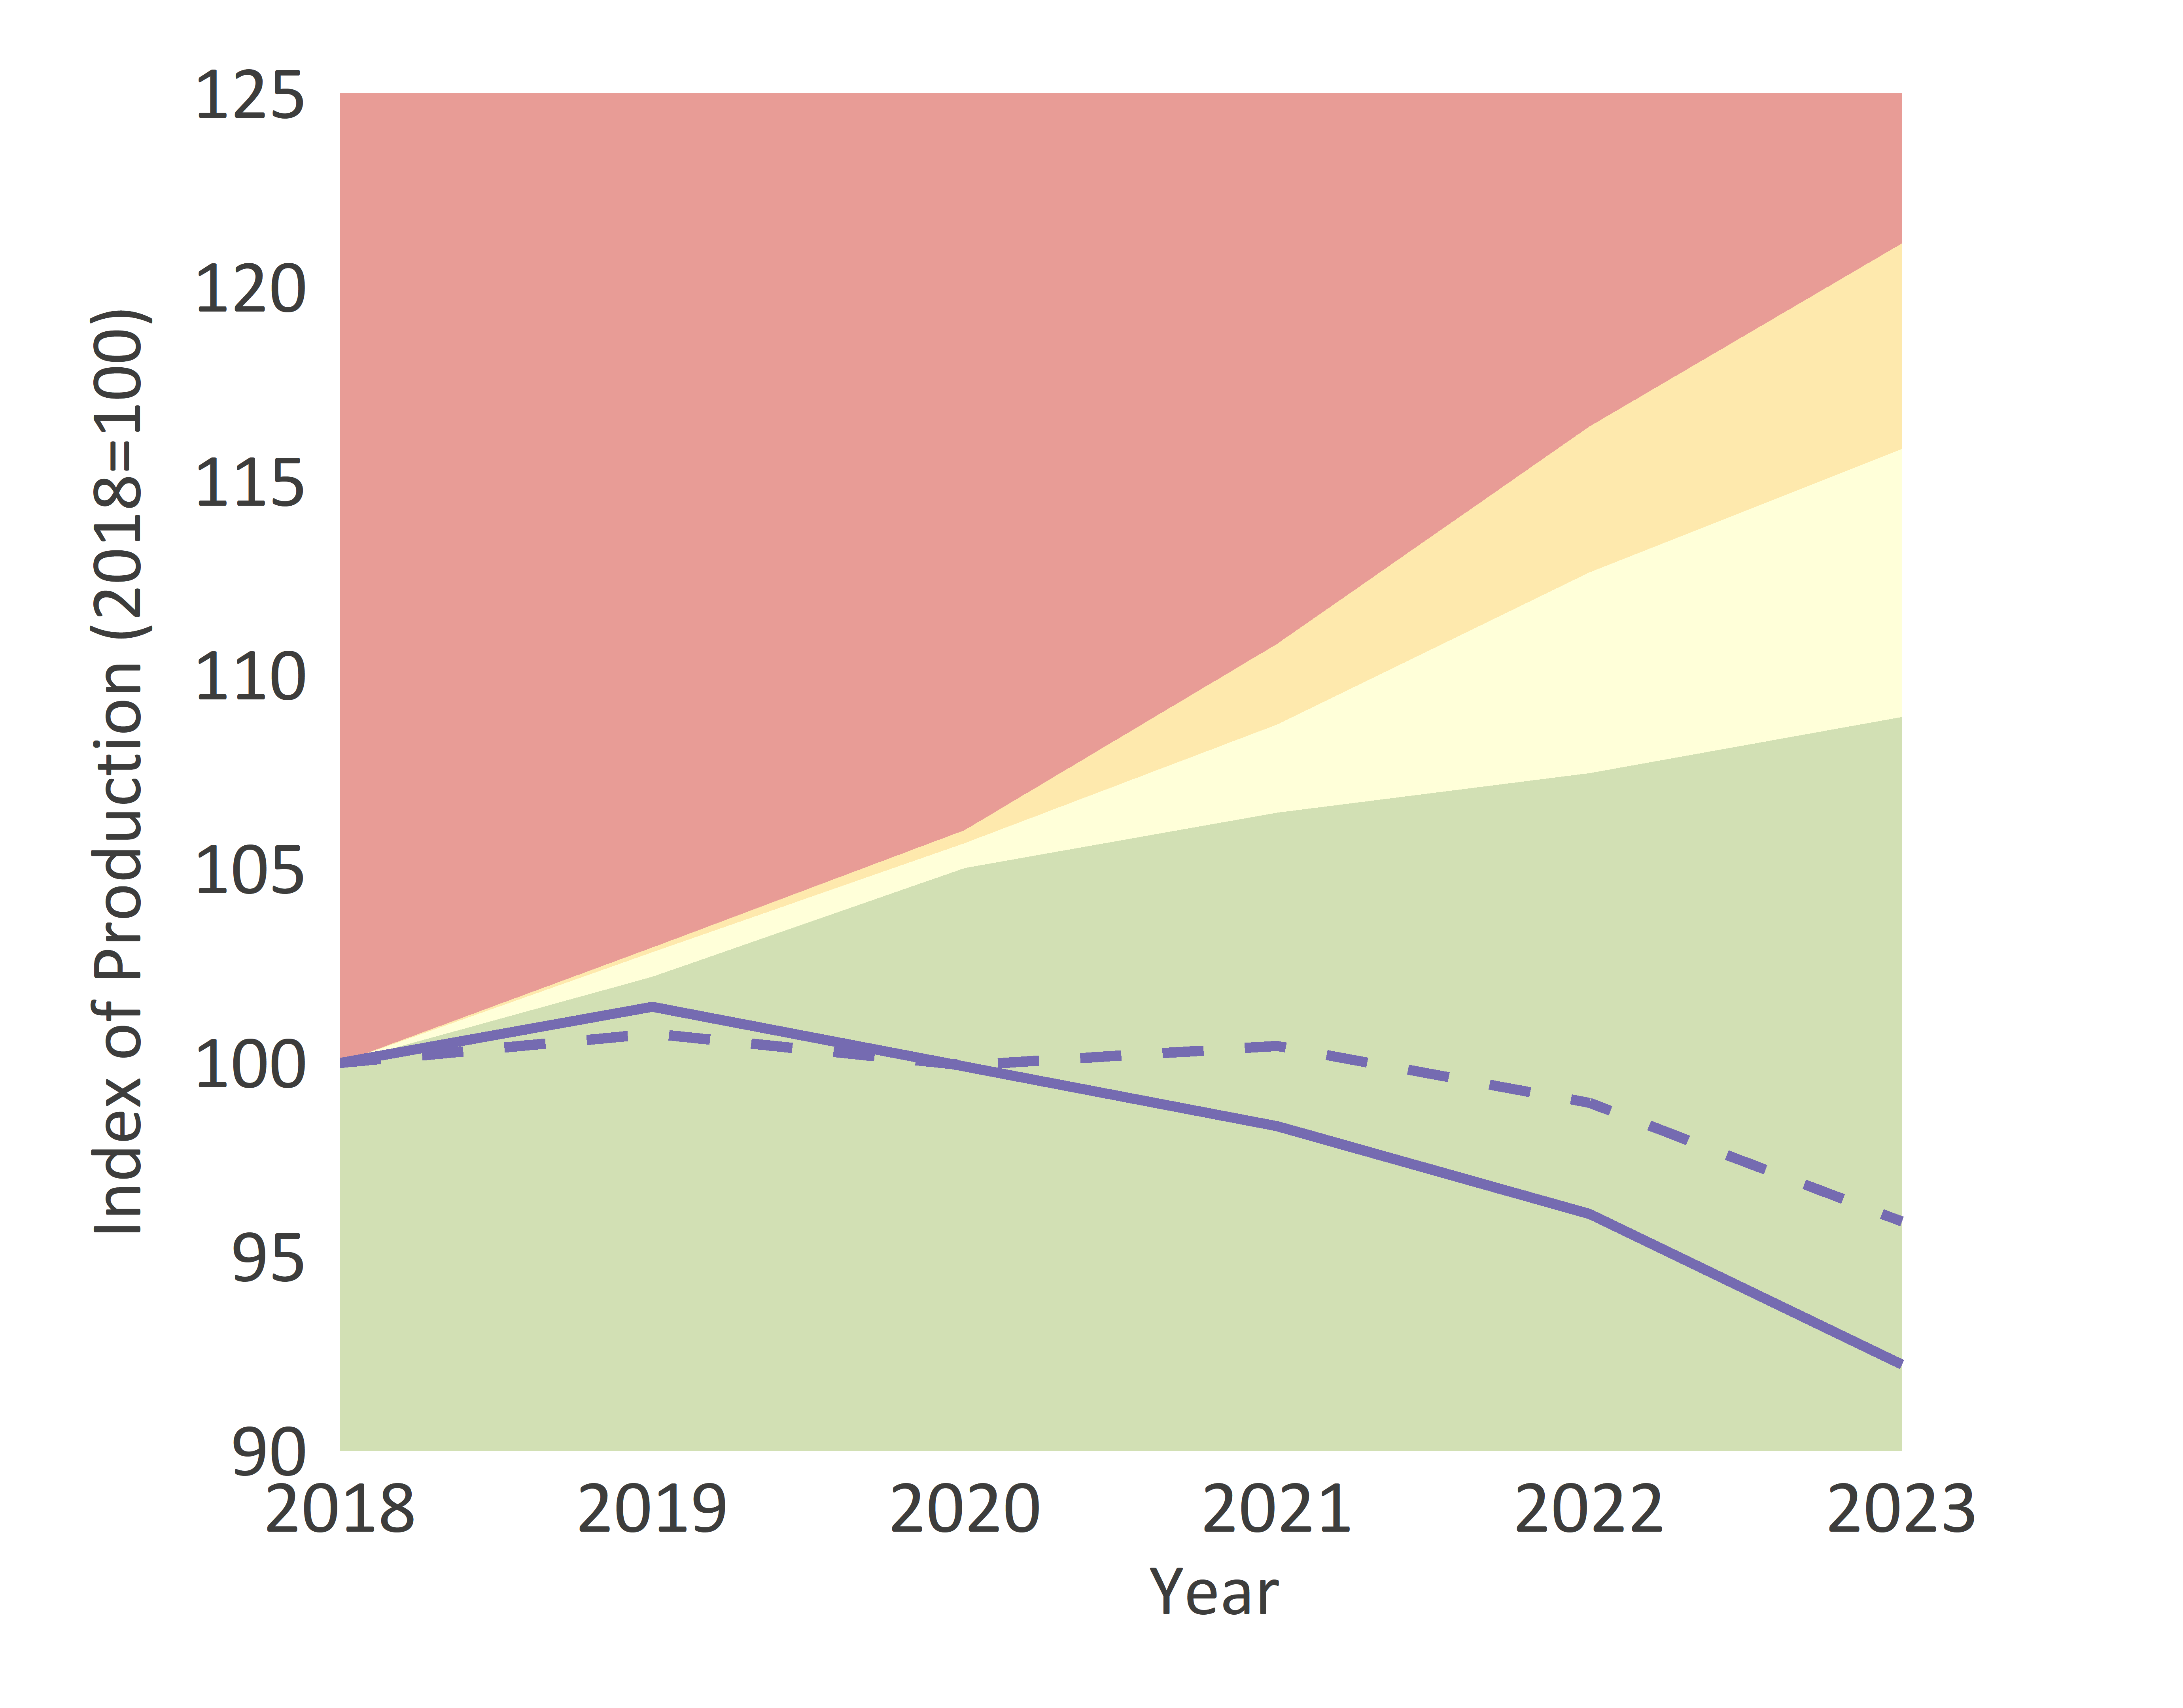
\includegraphics[trim = {0 0cm 0 0},width=1\linewidth]{Figures/Fig19}
			
		\end{minipage}
		
		
		\begin{center}
			\textbf{Automotive Sector}
		\end{center}
		
		\begin{minipage}[t]{.49\linewidth}
			\textbf{Trajectory of Combustion Engine Vehicle Production}
	
			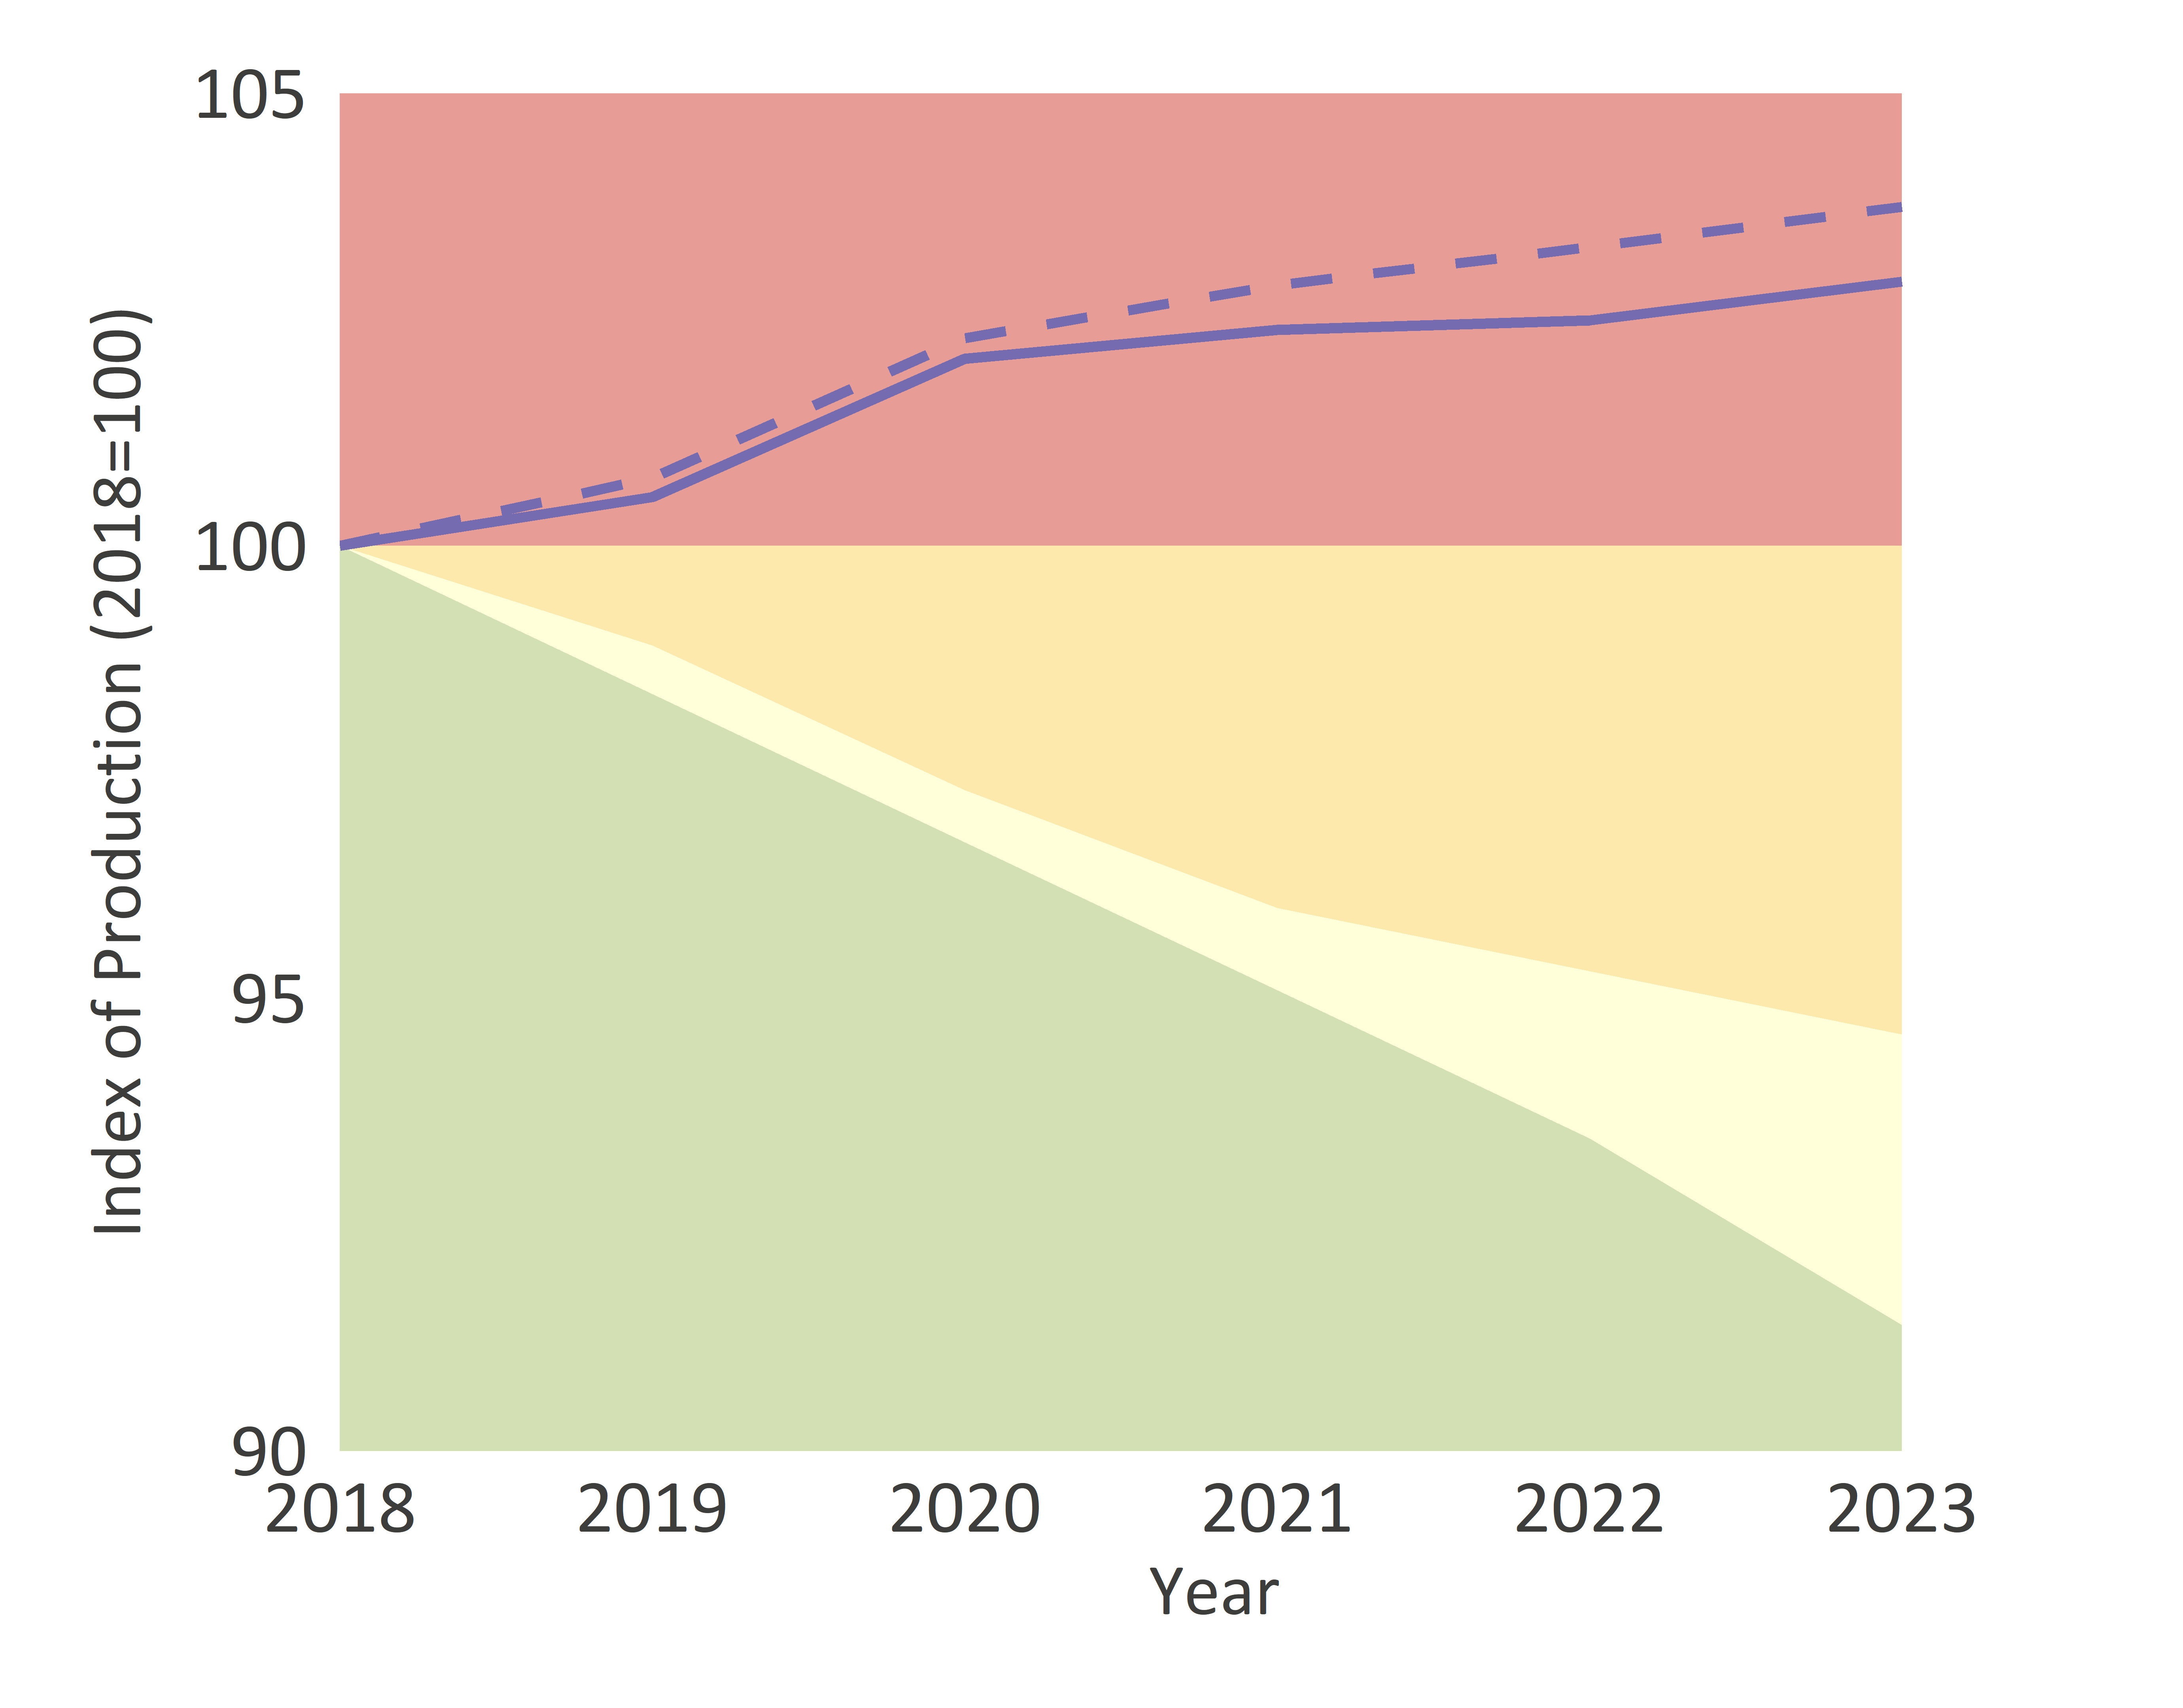
\includegraphics[trim = {0 0cm 0 0},width=1\linewidth]{Figures/Fig20}
			
		\end{minipage}	
		\hspace{.02\linewidth}
		\begin{minipage}[t]{.49\textwidth}
			\textbf{Trajectory of Electric Vehicle Production}
			
			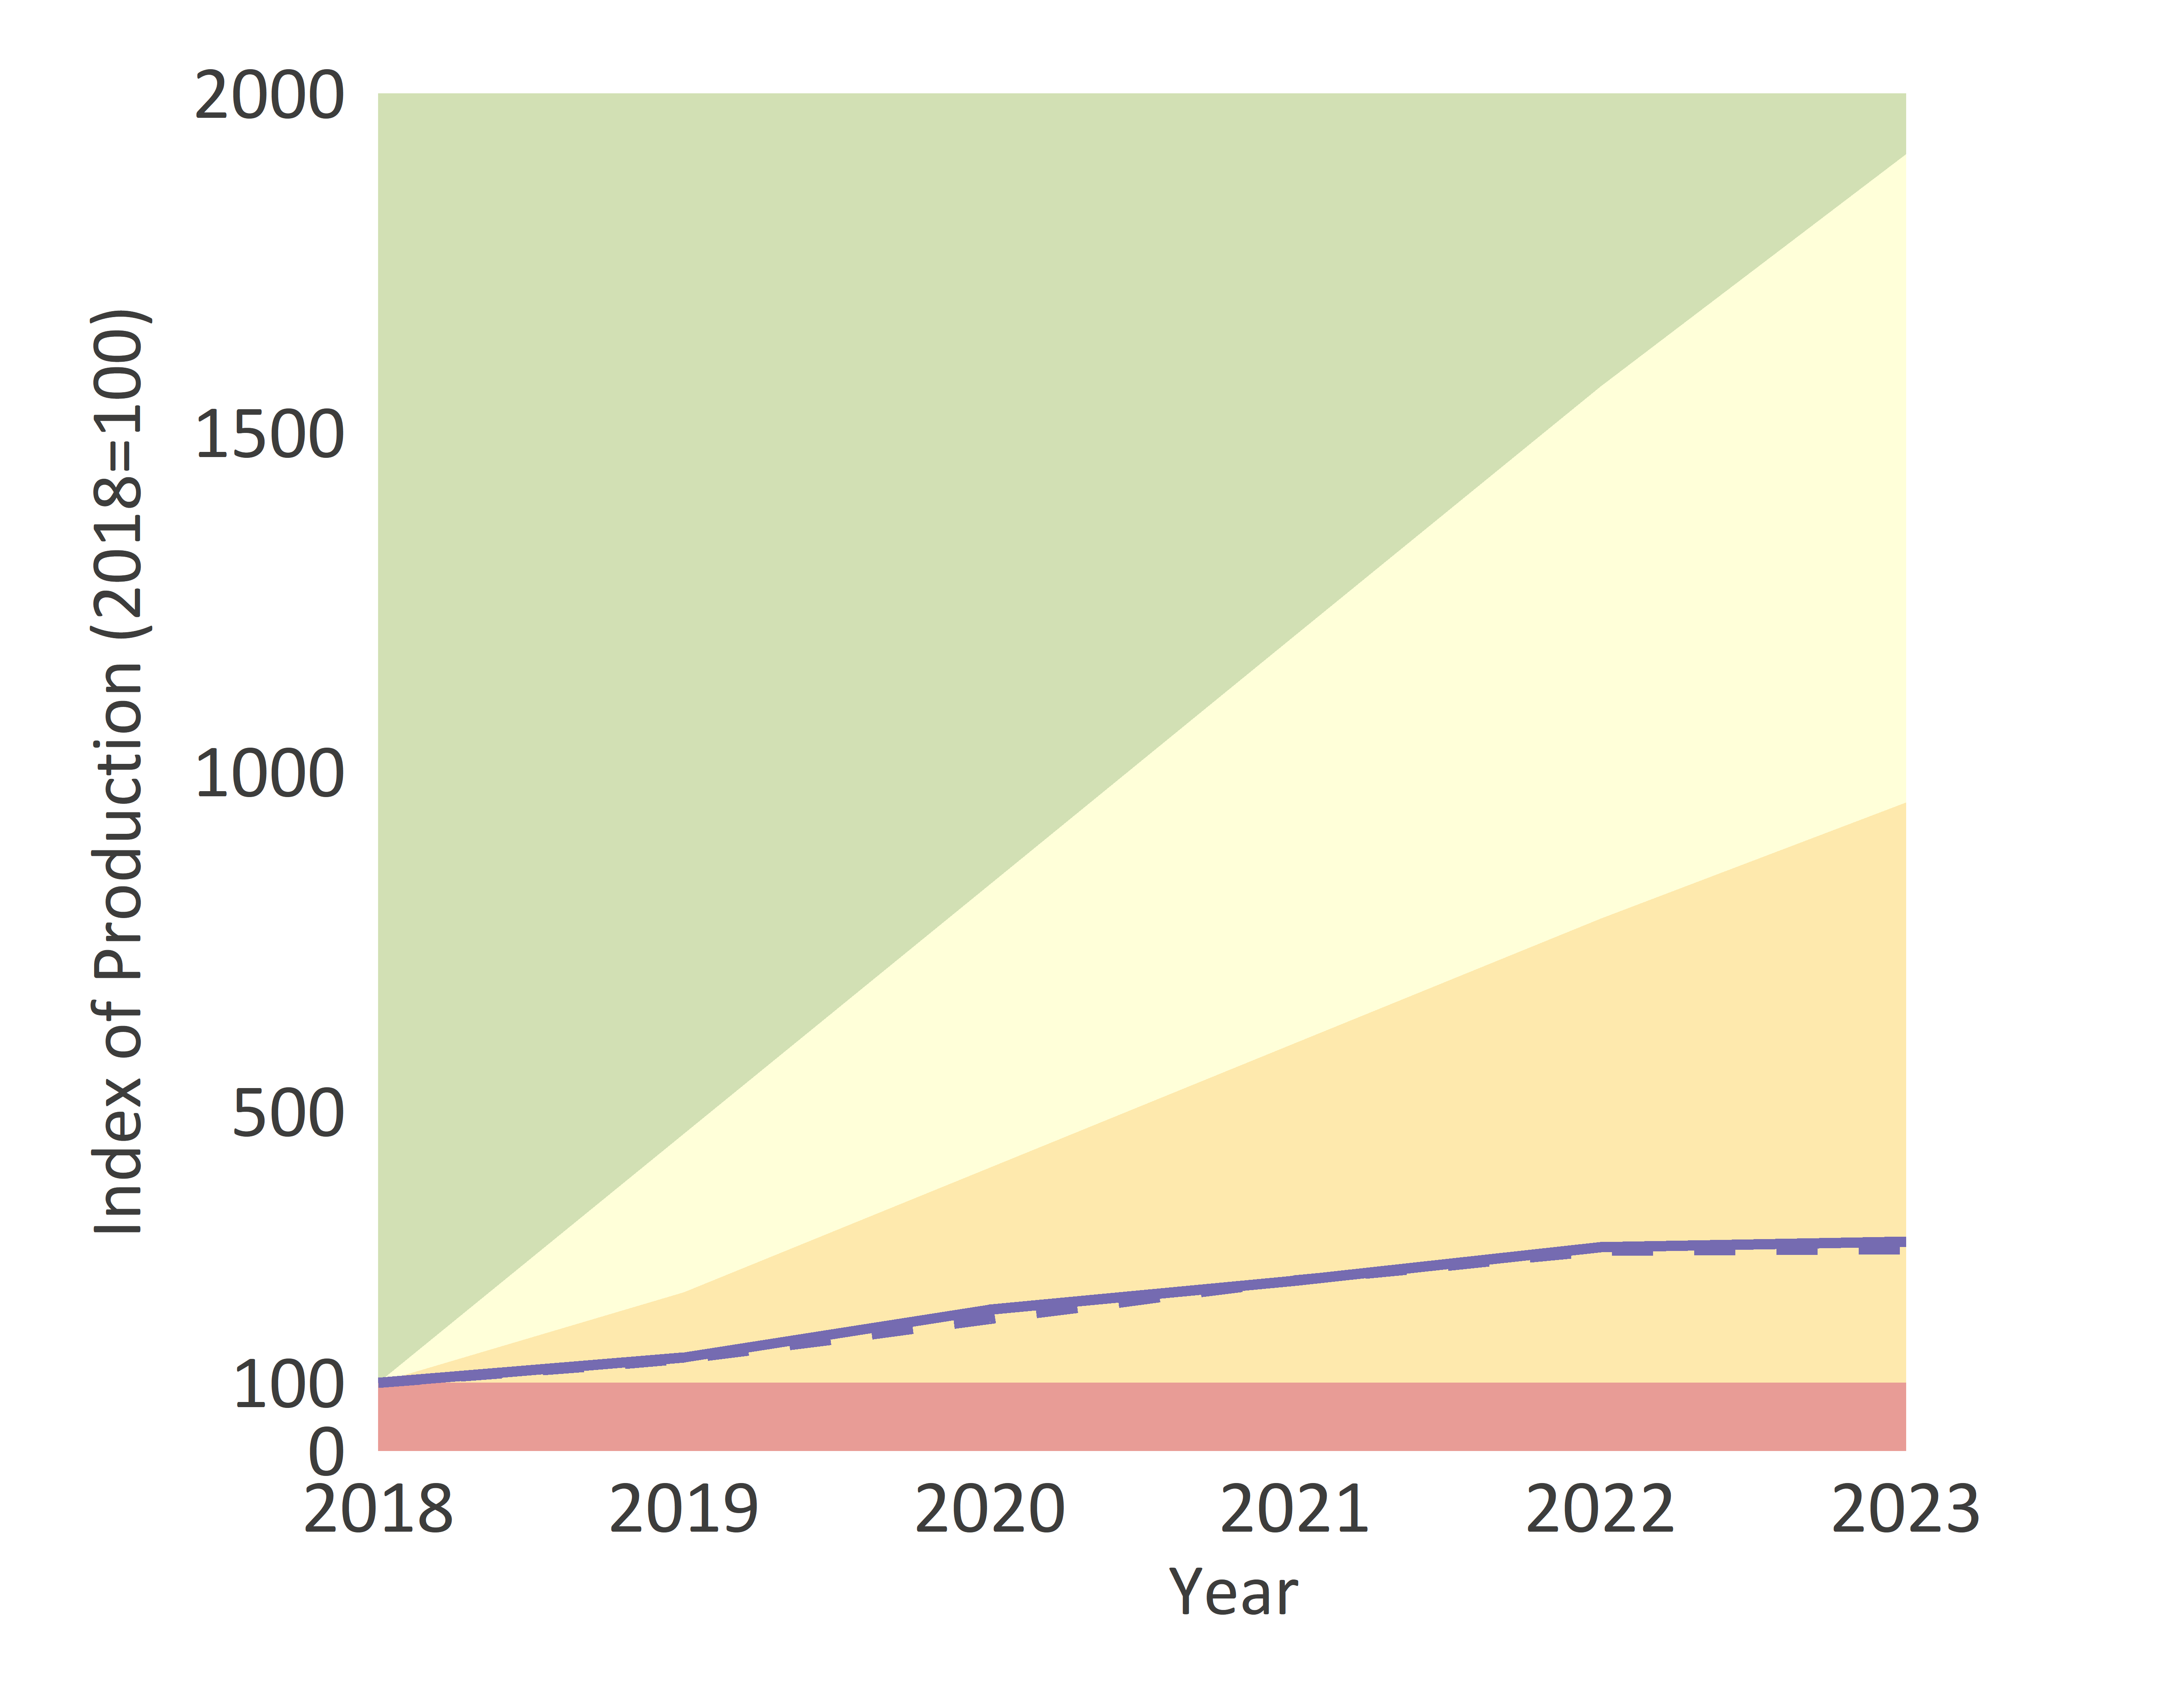
\includegraphics[trim = {0 0cm 0 0},width=1\linewidth]{Figures/Fig21}
			
		\end{minipage}		
		
		
		\begin{center}
			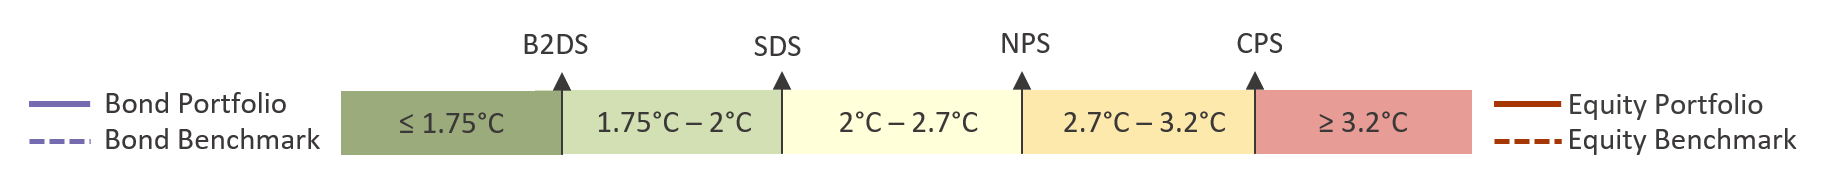
\includegraphics[trim = {0 0cm 0 0},width=.8\linewidth]{ReportGraphics/246Legend.png}
		\end{center}
		
	\PageFooterThird
	\newpage %CBSpecificE
		\section*{} % TRAJECTORY – EQUITY – POWER %EQSpecificS
	\HeaderDouble{5 YEAR TREND - EQUITY}{POWER}		
	
	\begin{multicols}{2}
		\textbf{The alignment graphs below show the alignment of selected power technologies in your equity portfolio relative to the IEA scenarios for 2°C, 4°C and 6°C temperature change, the global stock market and the average of the comparison group.} 
		
		These charts present the trajectory of buildout in the power sector for the companies with production within your equity portfolio. This has been normalized to the 2°C benchmark, so the plotted lines show the difference to a 2°C scenario outcome. This is overlayed over the different IEA scenarios for these technologies, represented by the shaded background. This shows how the buildout of capacity allocated to your portfolio is aligned to the scenarios.  The forward-looking estimates for your portfolio are based on asset-level data analysis by sector and technology provided by GlobalData for the power and fossil fuel sector, and WardsAuto / AutoForecastSolutions for the automobile sector. Further background information on the data sources can be found in Section 5. 
		
	\end{multicols}
	
	\vspace{-.4cm}	
	
	\begin{minipage}[t]{.49\linewidth}
		\textbf{Trajectory of Coal Power Capacity }
		
		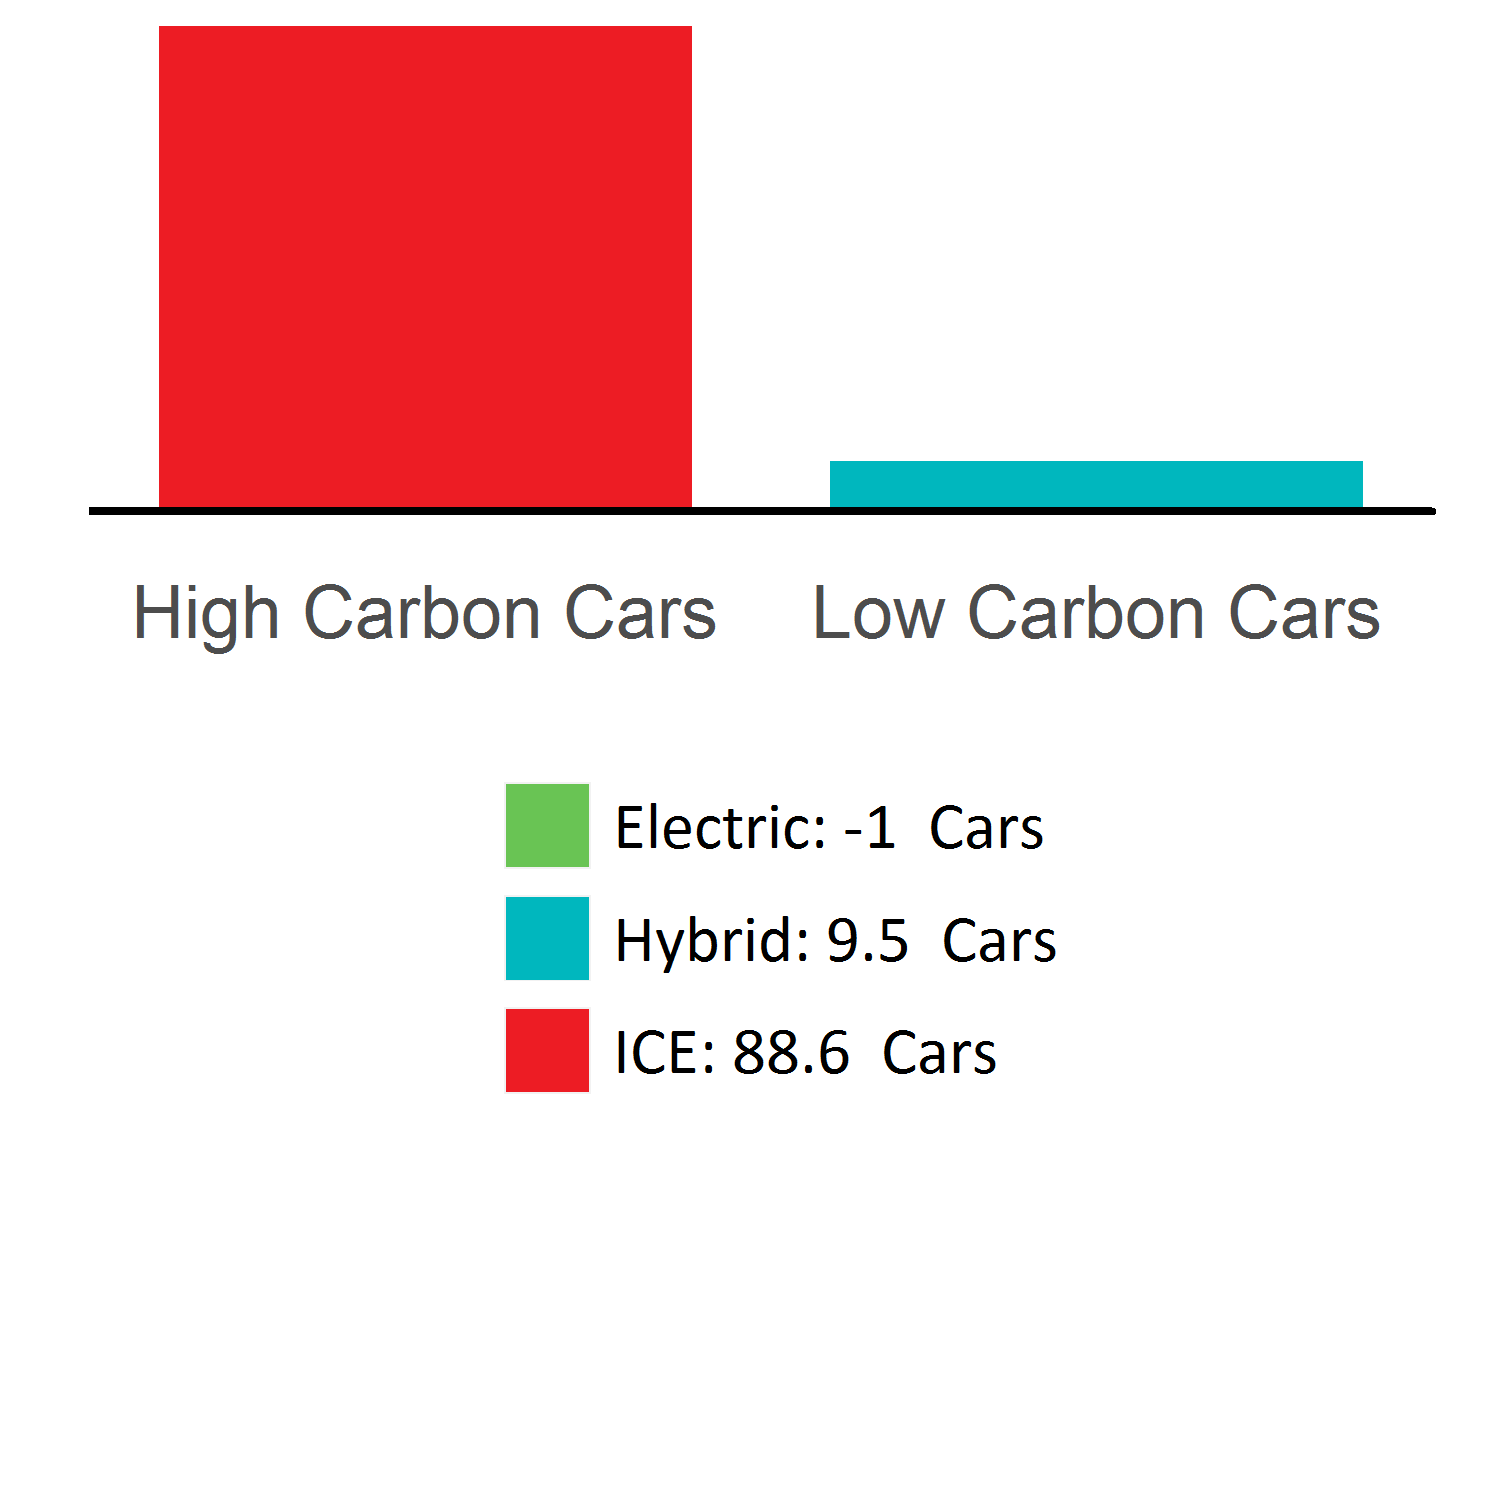
\includegraphics[trim = {0 0cm 0 0},width=1\linewidth]{Figures/Fig22}
		
		\textbf{Trajectory of Renewable Power Capacity }
		
		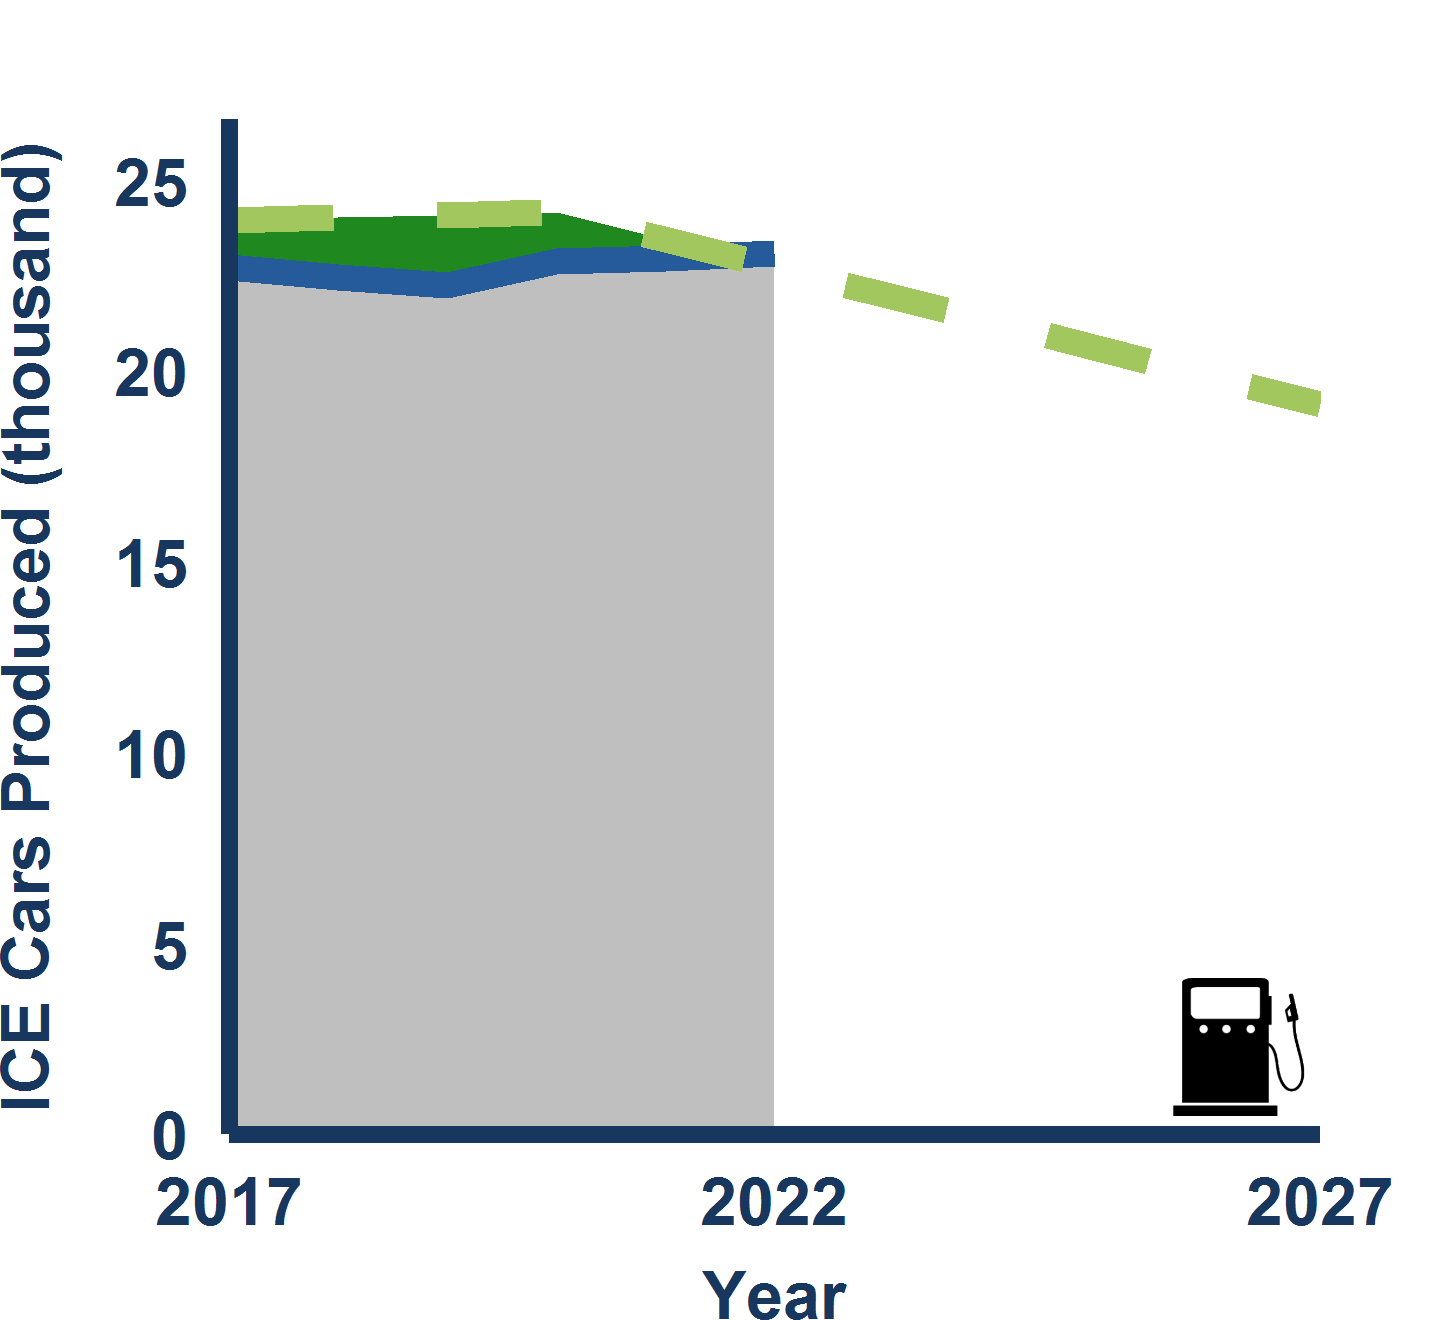
\includegraphics[trim = {0 0cm 0 0},width=.99\linewidth]{Figures/Fig23}
	\end{minipage}	
	\hspace{.02\linewidth}
	\begin{minipage}[t]{.49\textwidth}
		\textbf{Trajectory of Gas Power Capacity }
		
		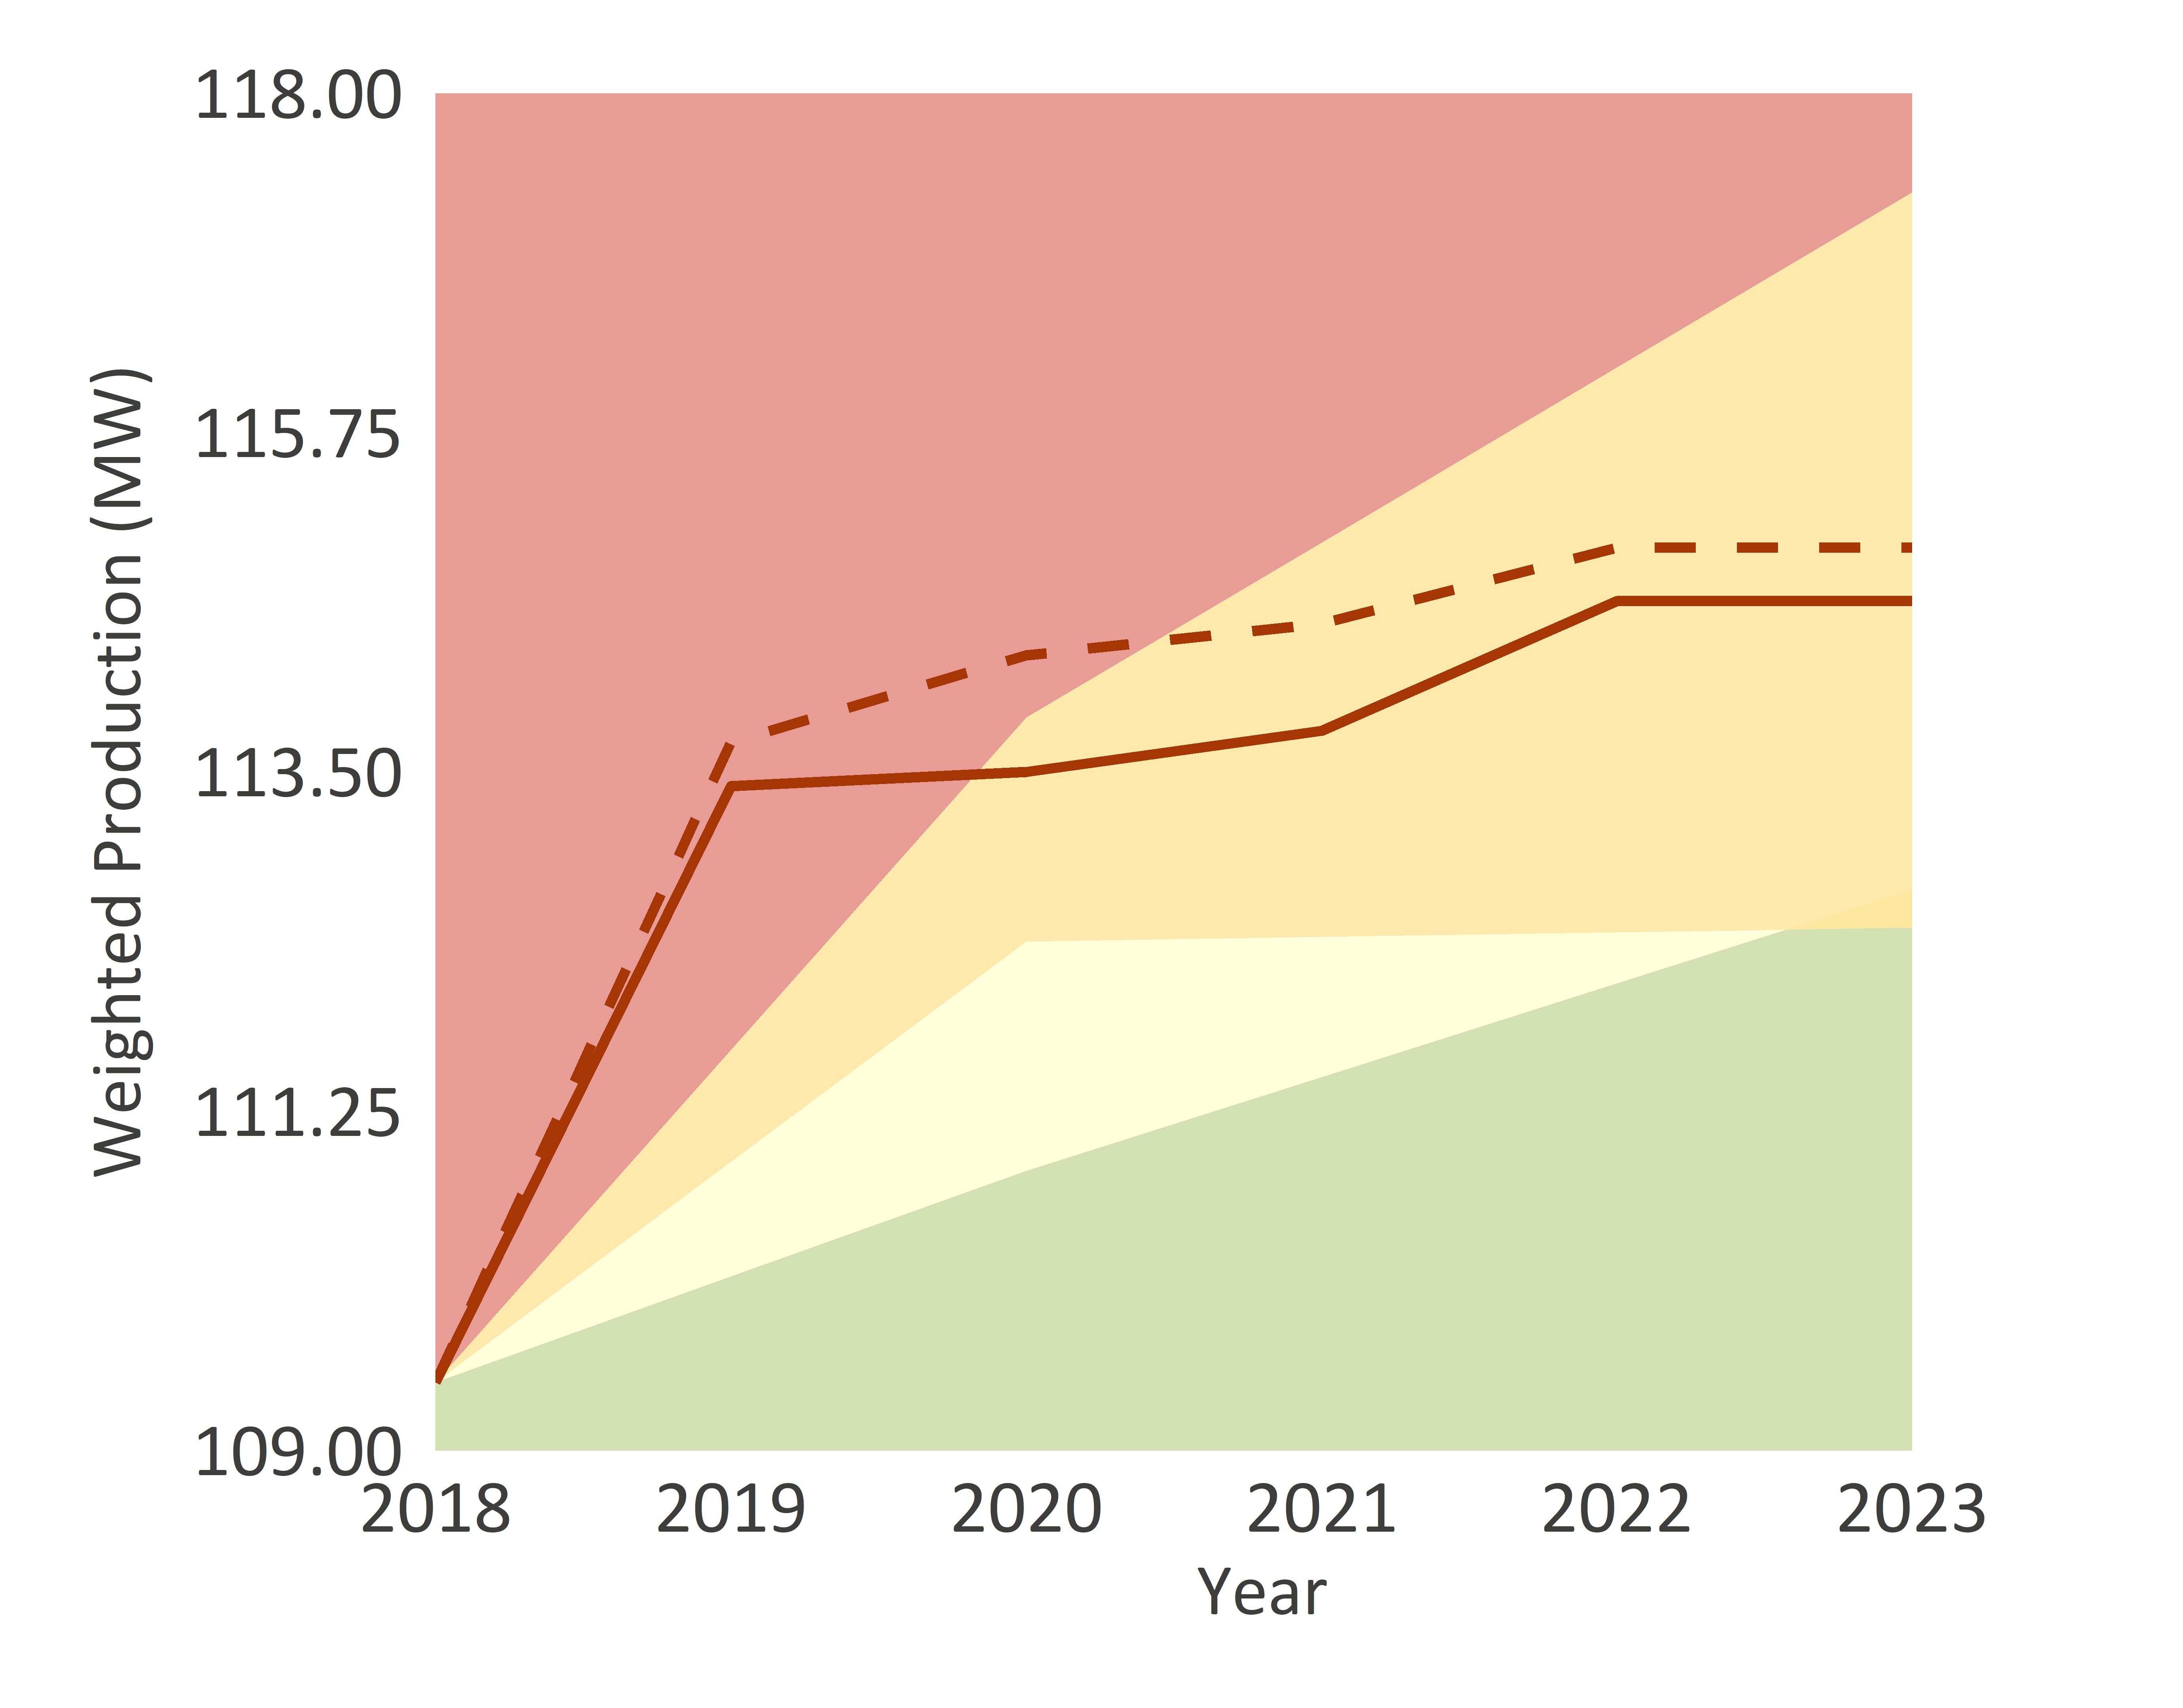
\includegraphics[trim = {0 0cm 0 0},width=1\linewidth]{Figures/Fig24}
		
		\textbf{Trajectory of Nuclear Power Capacity }
		
		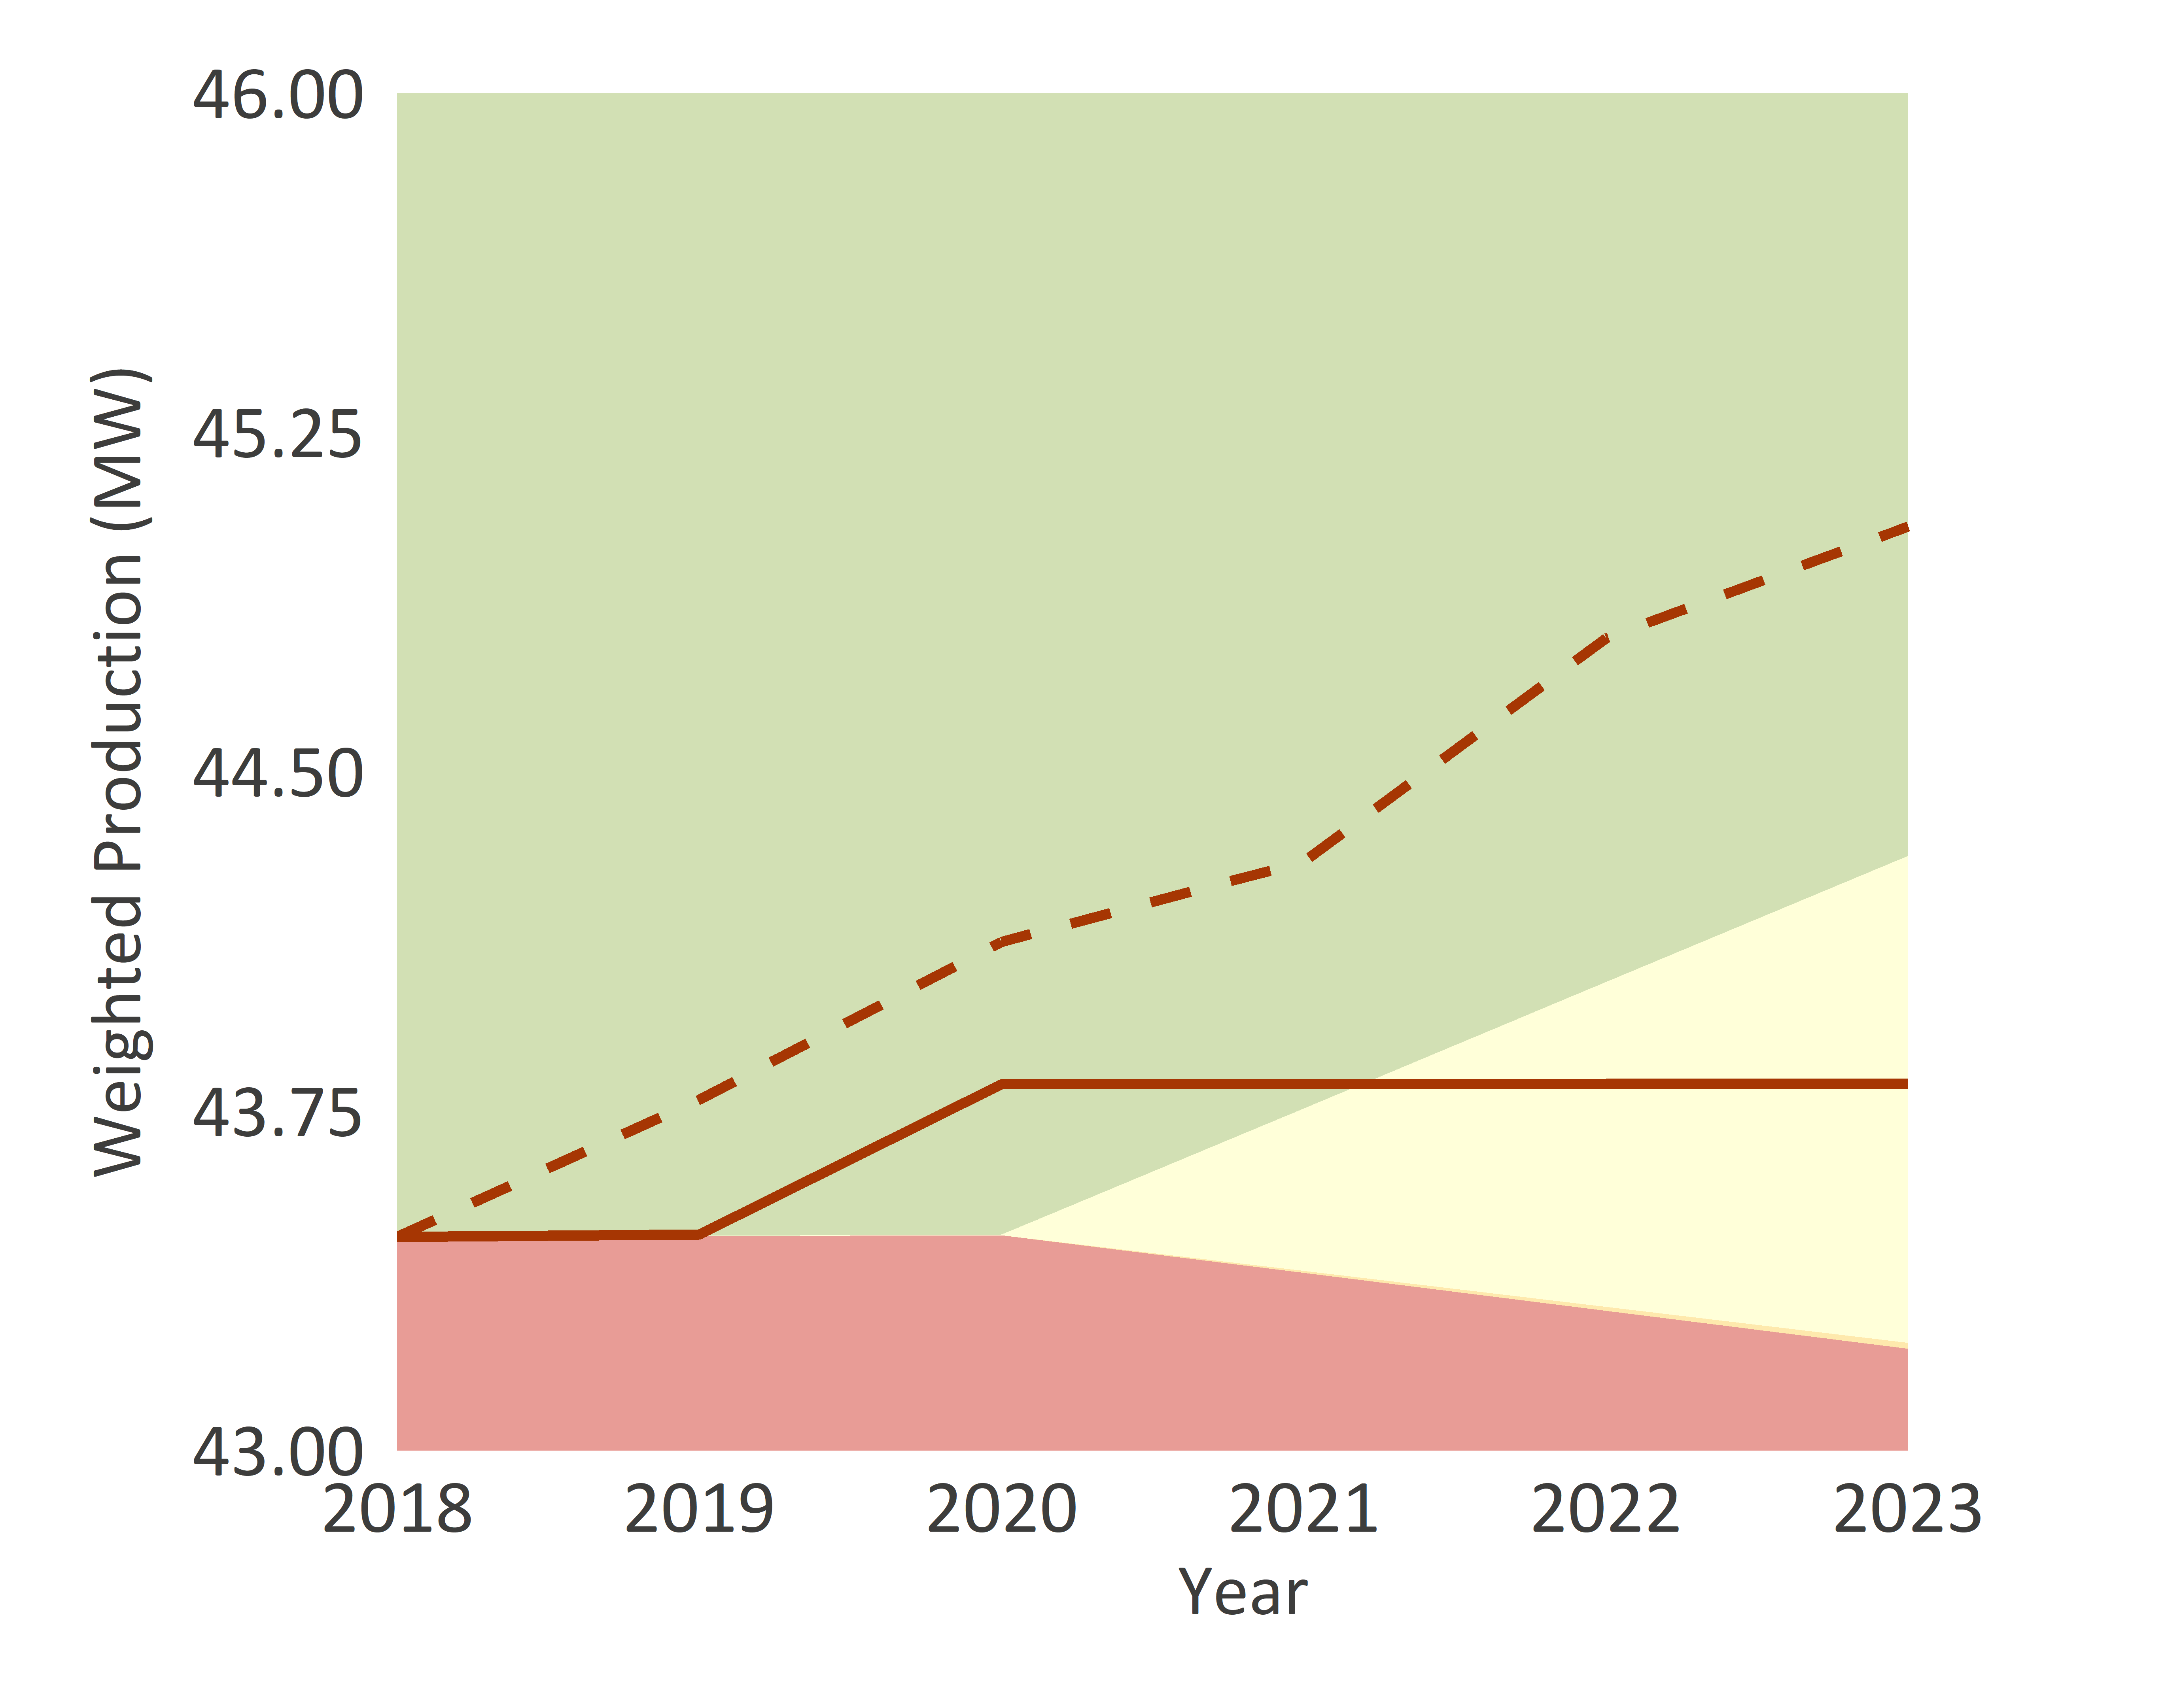
\includegraphics[trim = {0 0cm 0 0},width=1\linewidth]{Figures/Fig25}
		
	\end{minipage}
	
	\vspace{-0.4cm}
	\begin{center}
		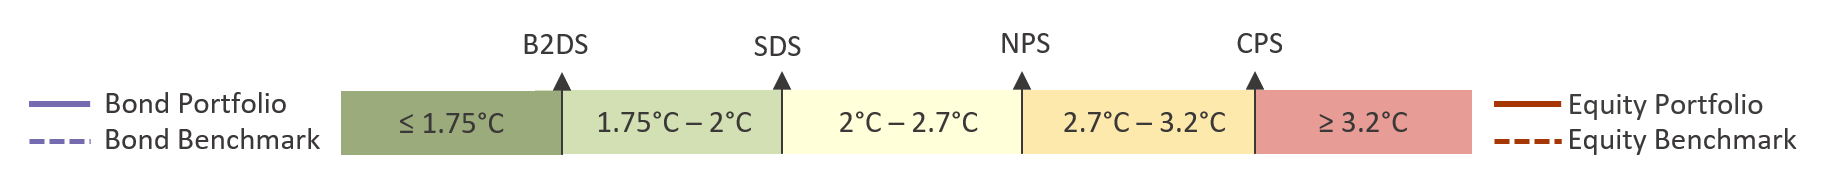
\includegraphics[trim = {0 0cm 0 0},width=.8\linewidth]{ReportGraphics/246Legend.png}
	\end{center}
	
	
	\PageFooterThird
	\newpage 
	\section*{} % TRAJECTORY – EQUITY – FOSSIL FUELS AND AUTOMOTIVE  
	\HeaderDouble{5 YEAR TREND - EQUITY}{FOSSIL FUELS AND AUTOMOTIVE}	
	
	\begin{multicols}{2}
		\textbf{The alignment graphs below show the alignment of selected fossil fuels and automobile technologies in your equity portfolio relative to the IEA scenarios for 2°C, 4°C and 6°C temperature change, the global stock market and the average of the comparison group. } 
		
		The page brings together data on the upstream supply of fossil fuels and the largest downstream user of oil, namely the automotive sector. It highlights the extent to which within a portfolio the strategies across sectors may be more or less consistent, relative to a 2°C scenario.
		
	\end{multicols}		
	
	\begin{center}
		\textbf{Fossil Fuel Sector}
	\end{center}
	
	\begin{minipage}[t]{.49\linewidth}
		\textbf{Trajectory of Oil Production }
		
		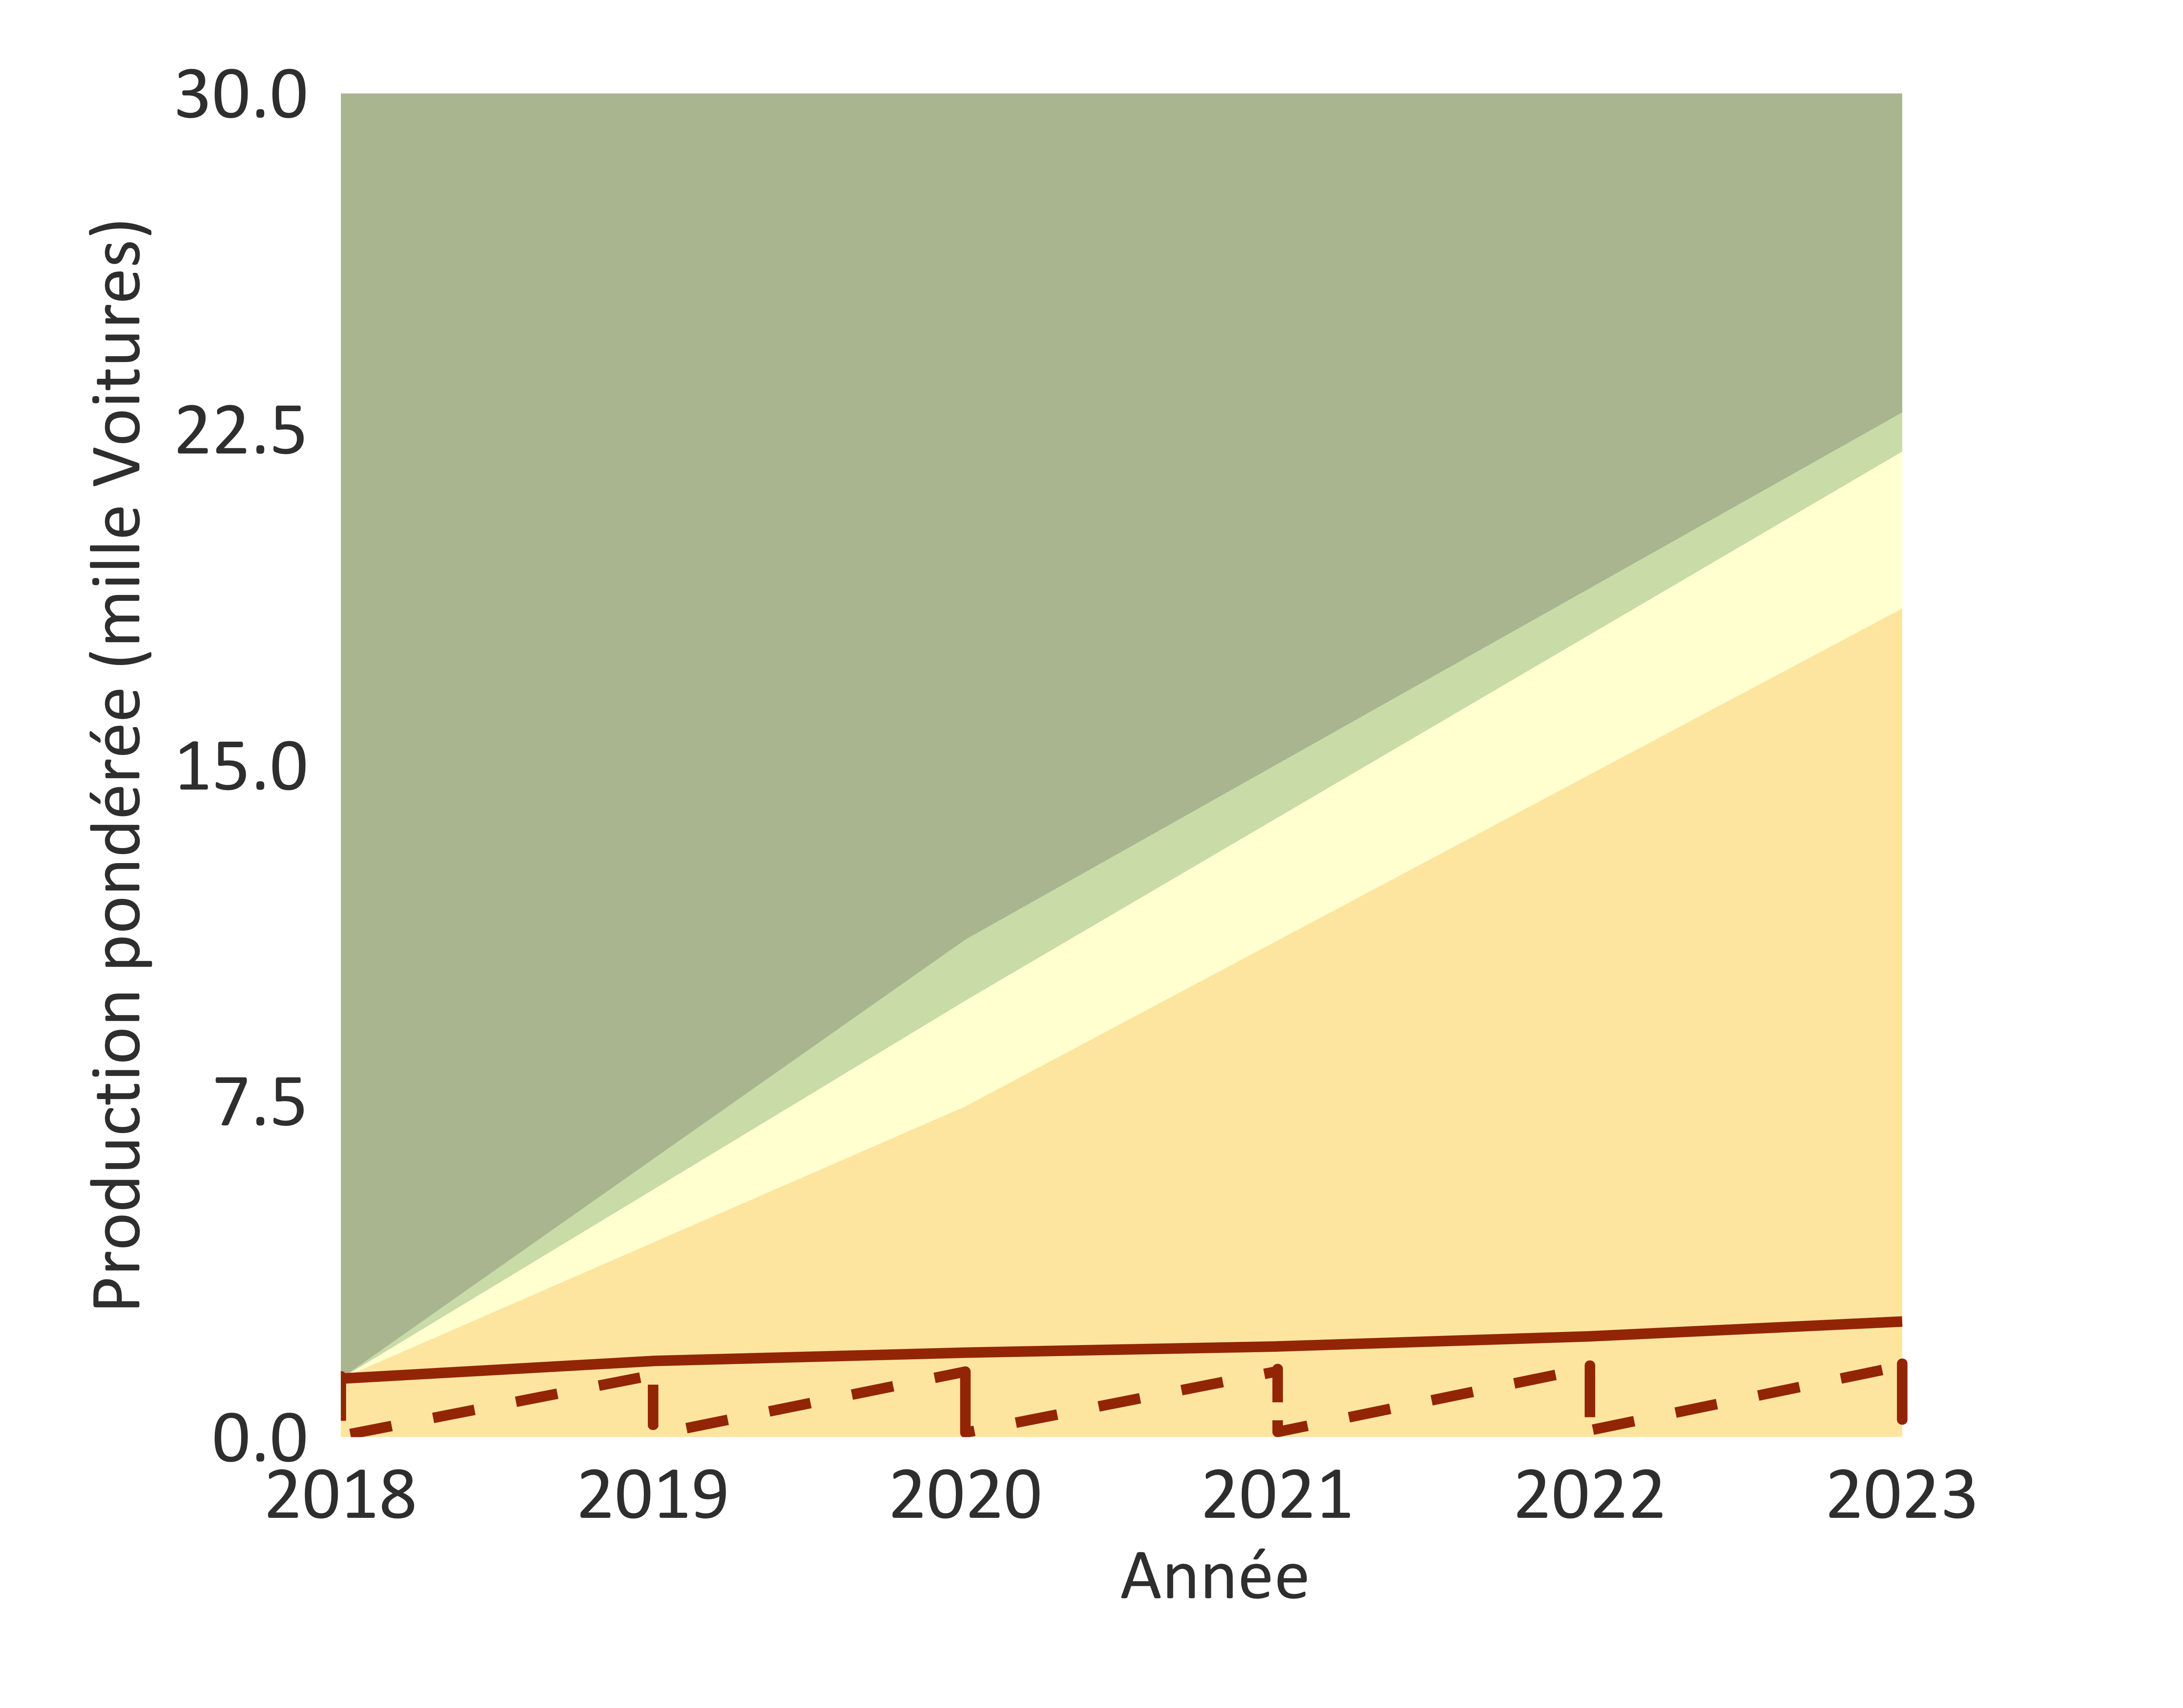
\includegraphics[trim = {0 0cm 0 0},width=1\linewidth]{Figures/Fig26}
		
	\end{minipage}	
	\hspace{.02\linewidth}
	\begin{minipage}[t]{.49\textwidth}
		\textbf{Trajectory of Gas Production }
		
		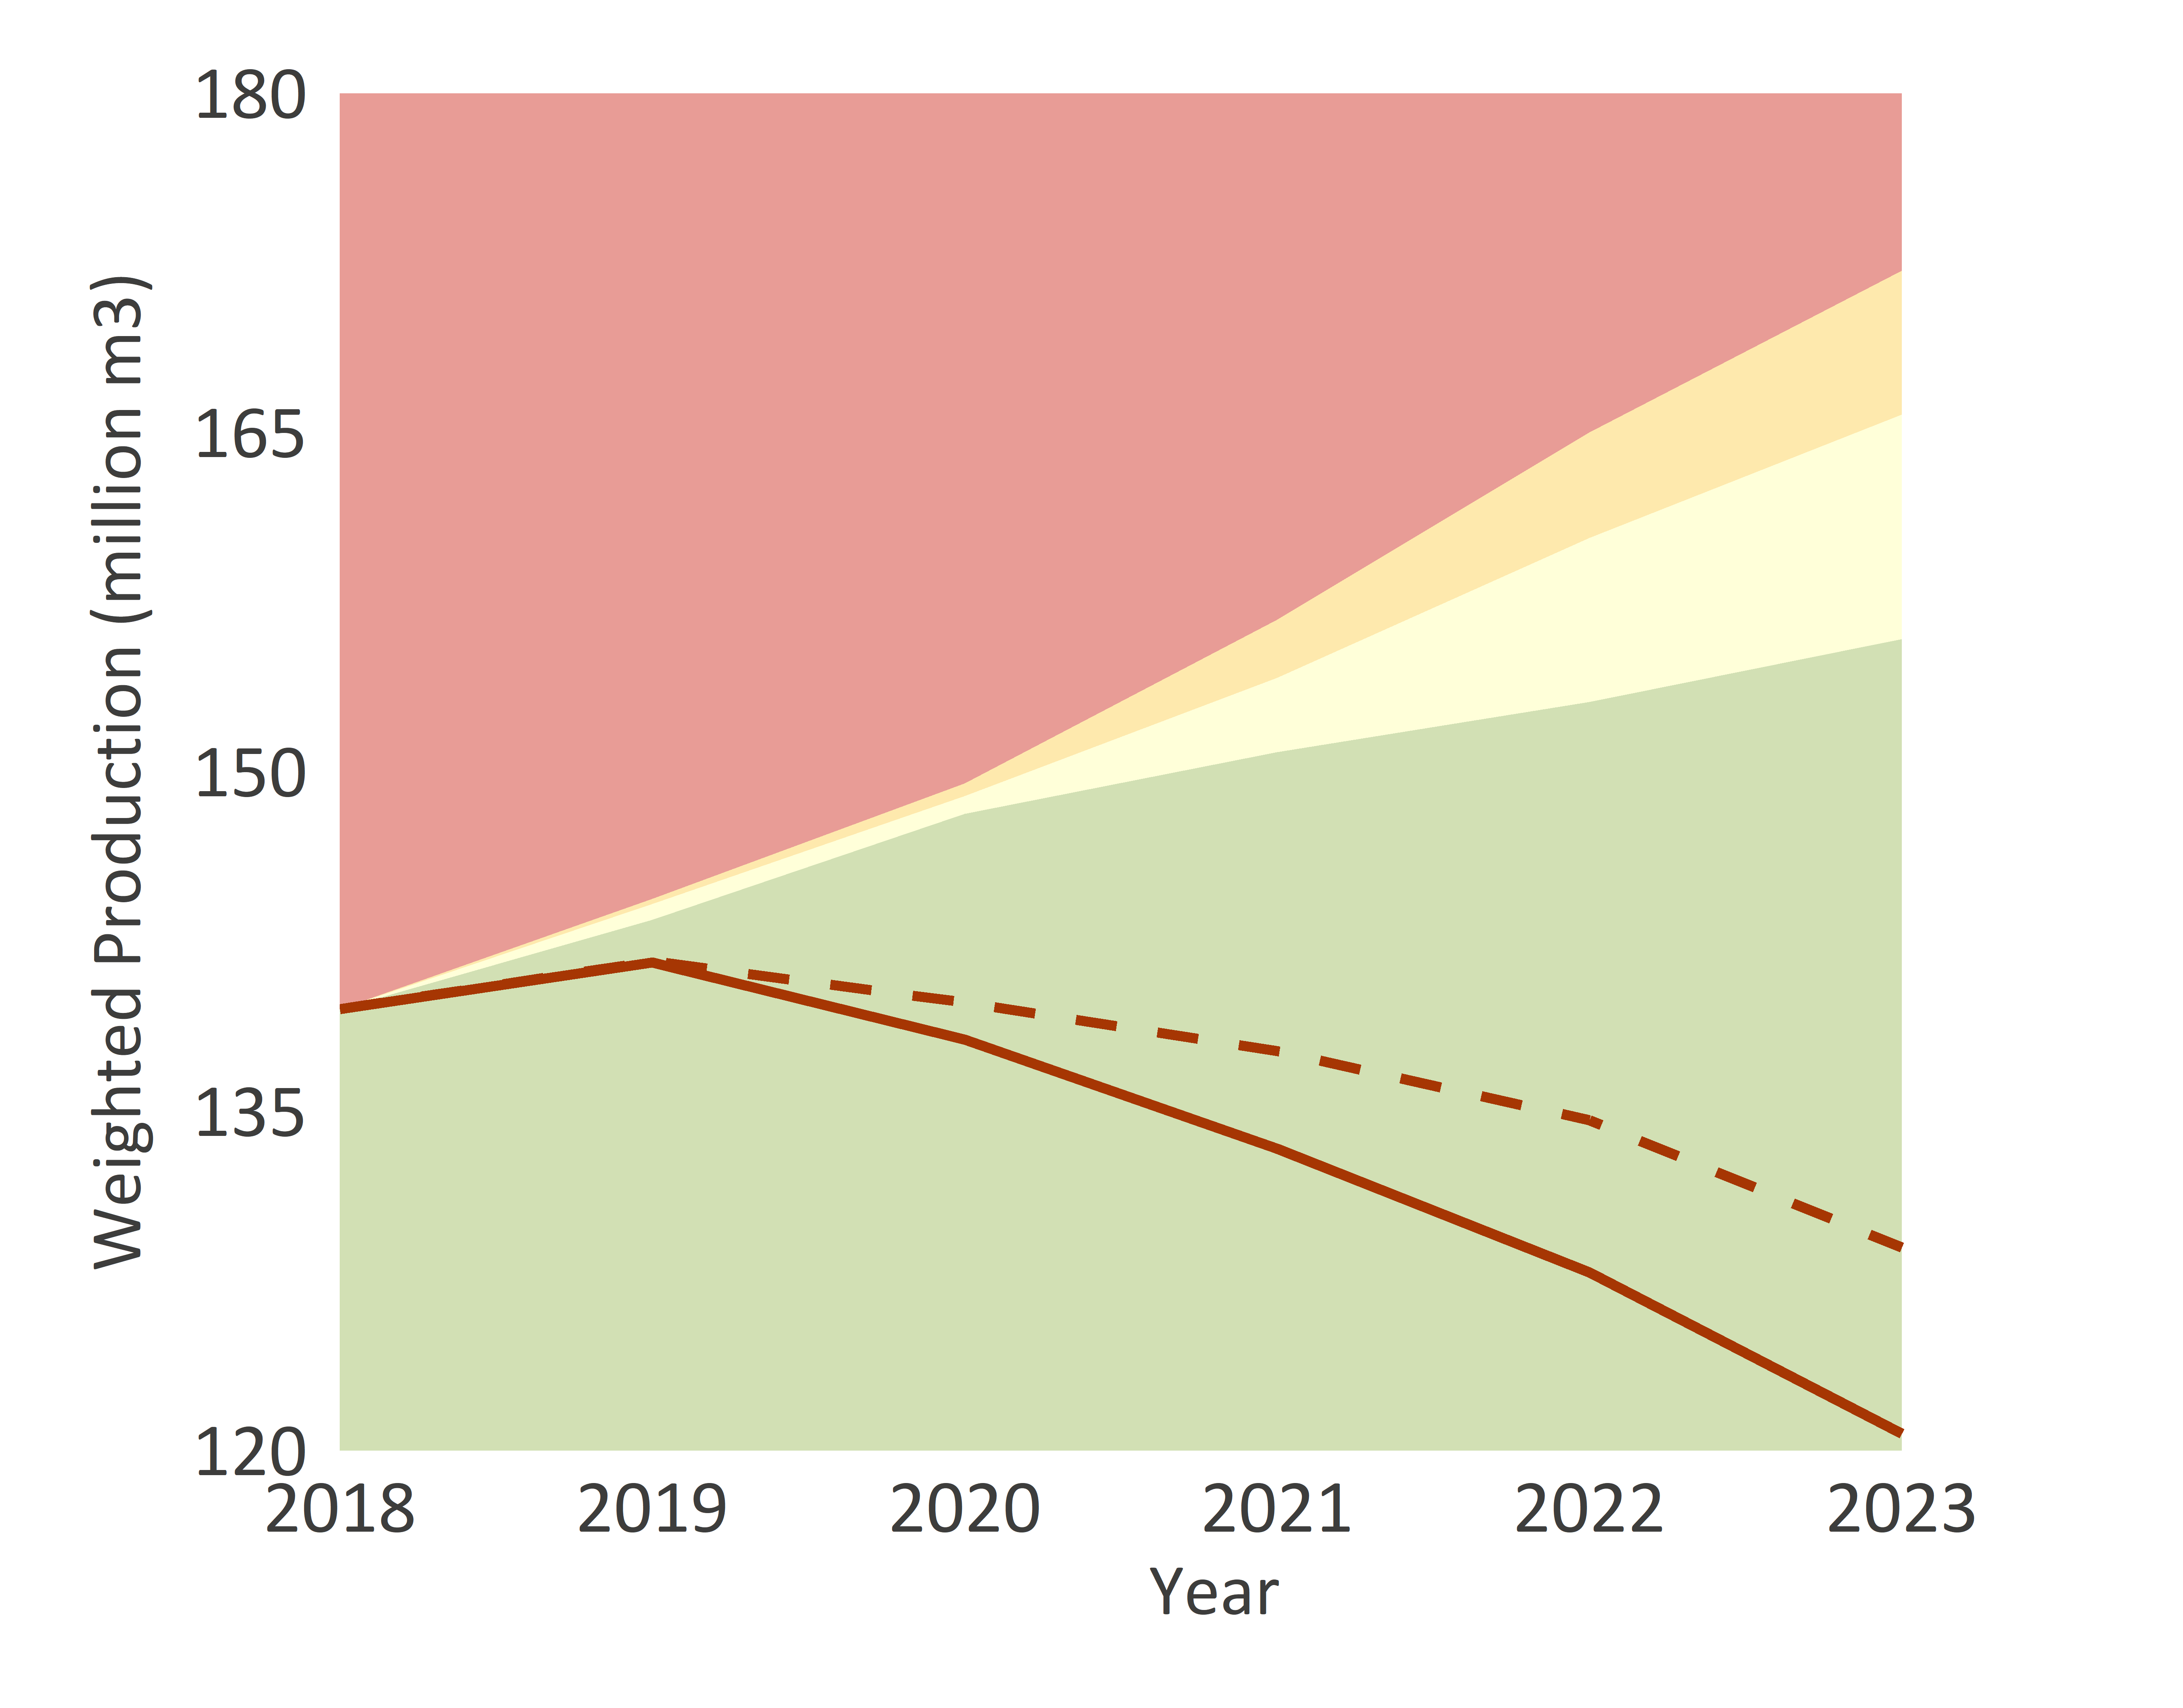
\includegraphics[trim = {0 0cm 0 0},width=1\linewidth]{Figures/Fig27}
		
	\end{minipage}
	
	
	\begin{center}
		\textbf{Automotive Sector}
	\end{center}
	
	\begin{minipage}[t]{.49\linewidth}
		\textbf{Trajectory of Combustion Engine Vehicle Production}
		
		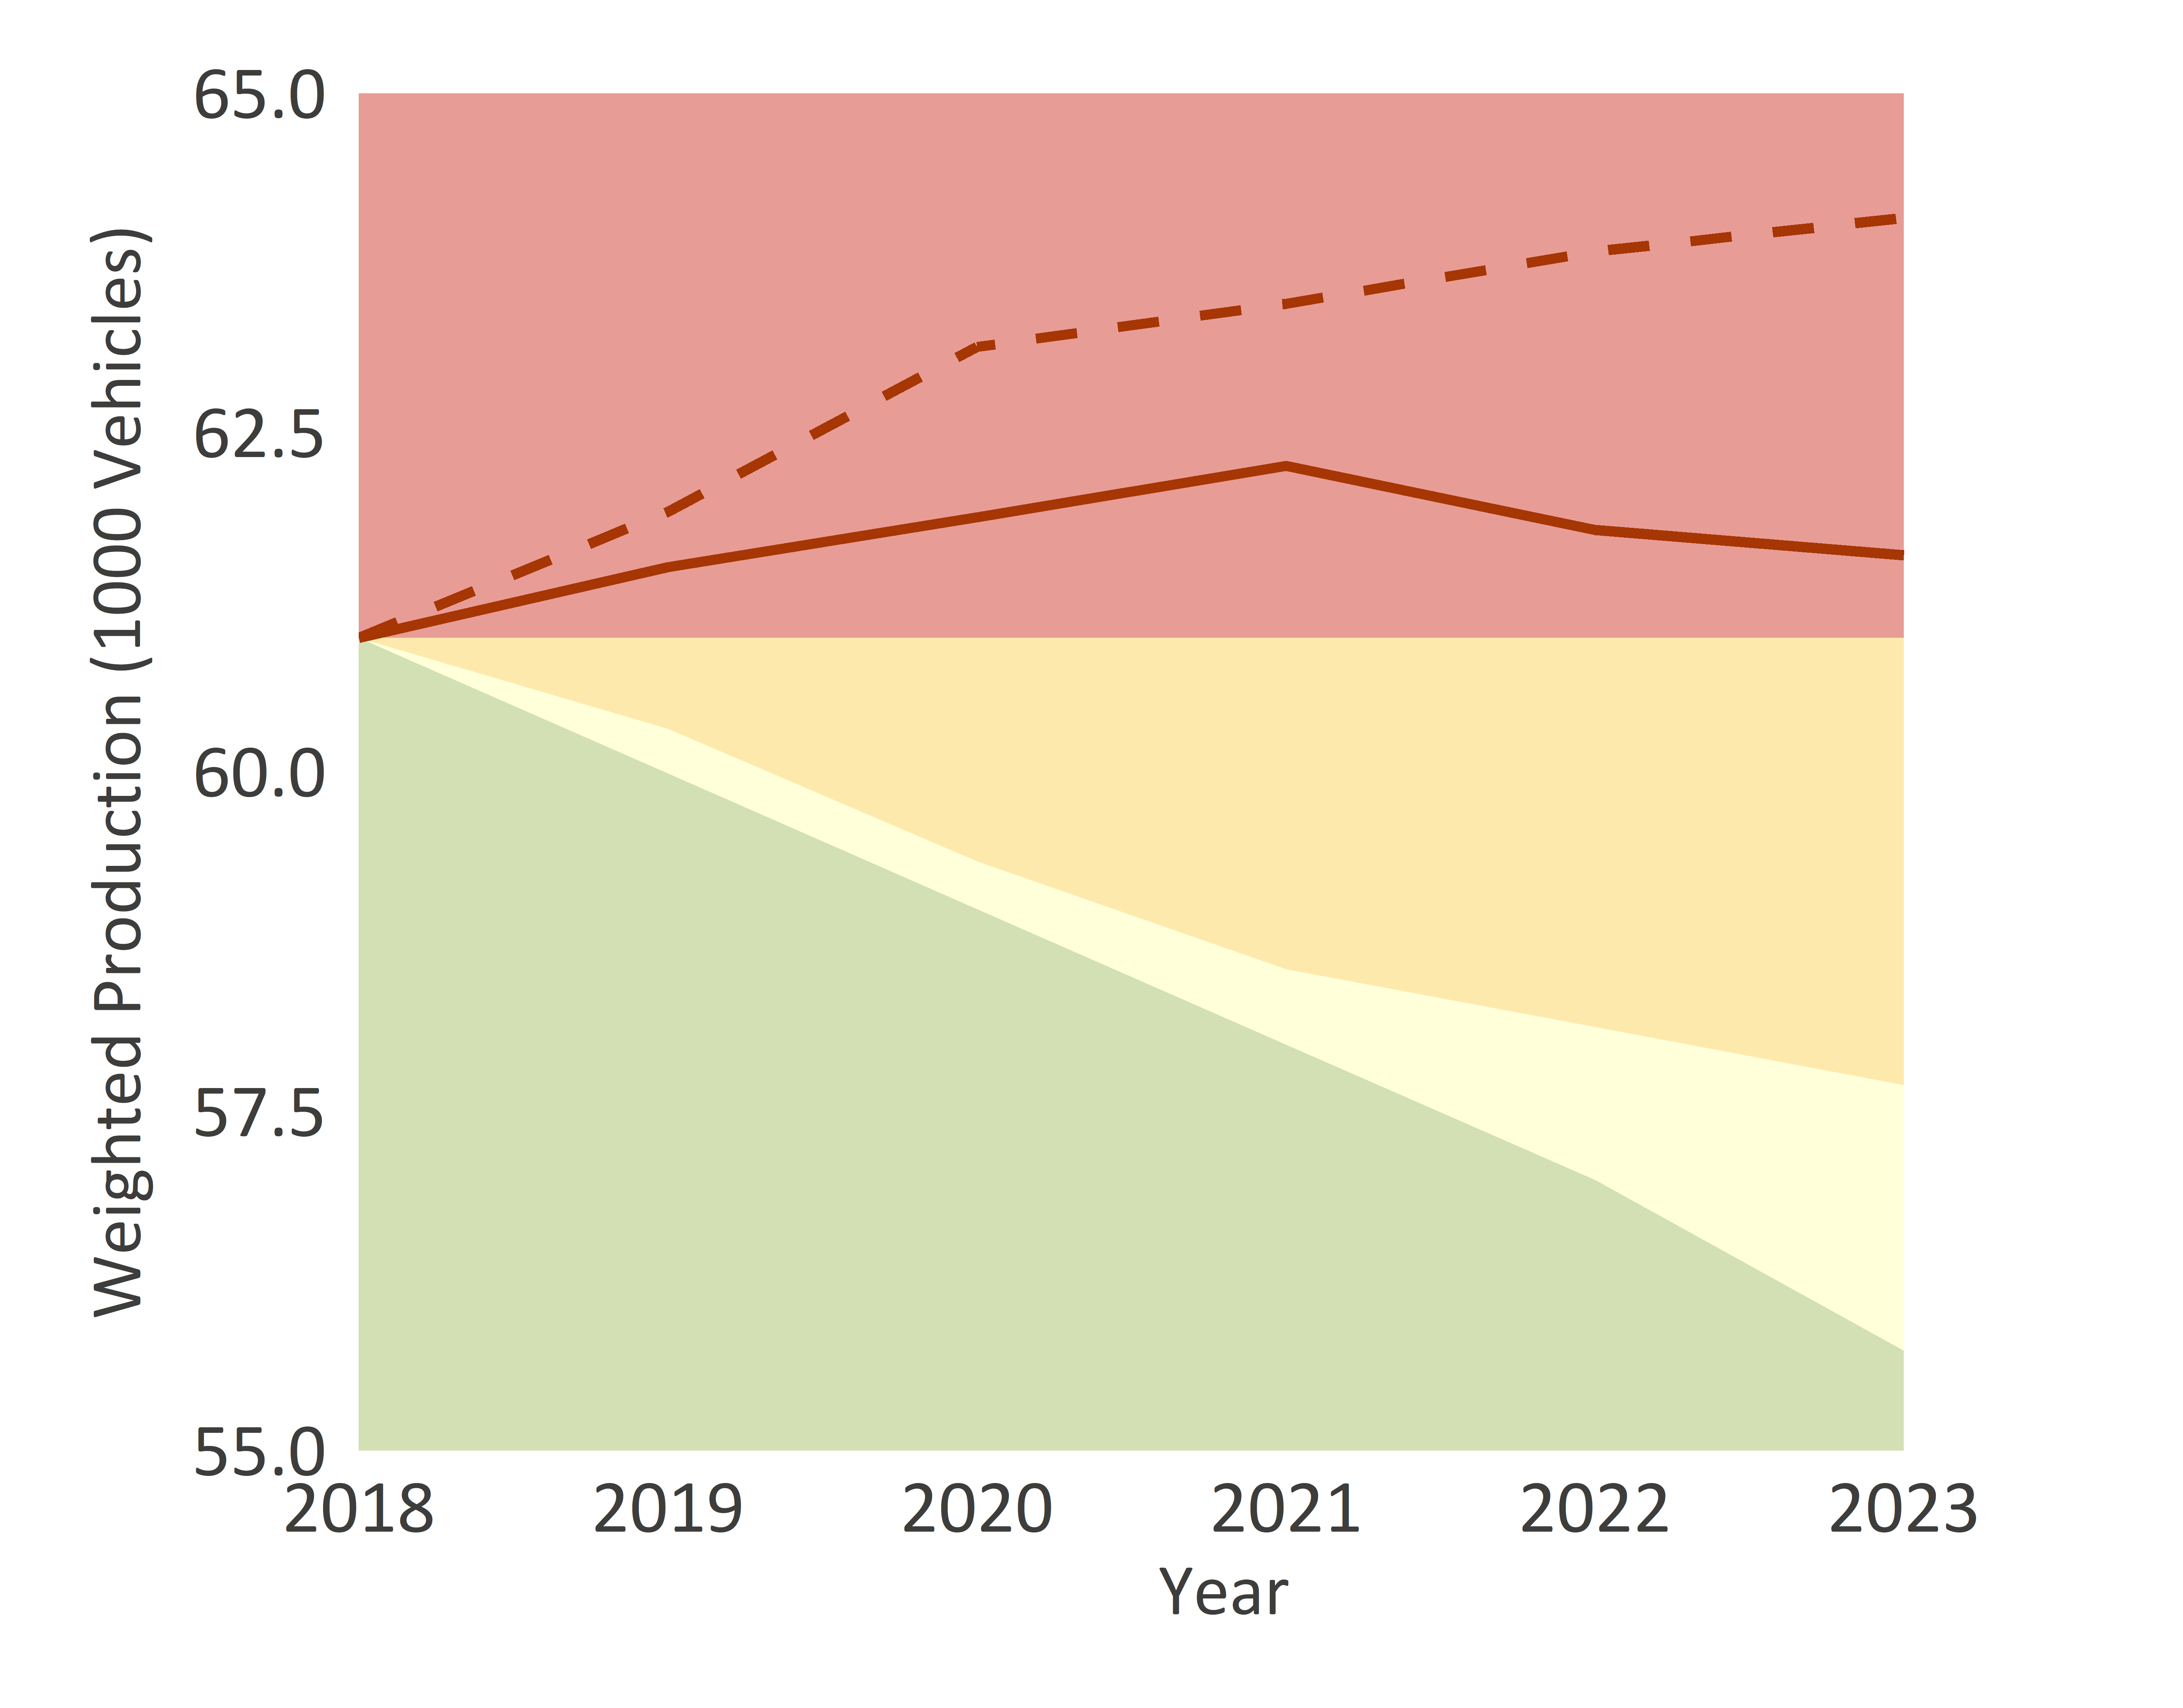
\includegraphics[trim = {0 0cm 0 0},width=1\linewidth]{Figures/Fig28}
		
	\end{minipage}	
	\hspace{.02\linewidth}
	\begin{minipage}[t]{.49\textwidth}
		\textbf{Trajectory of Electric Vehicle Production}
		
		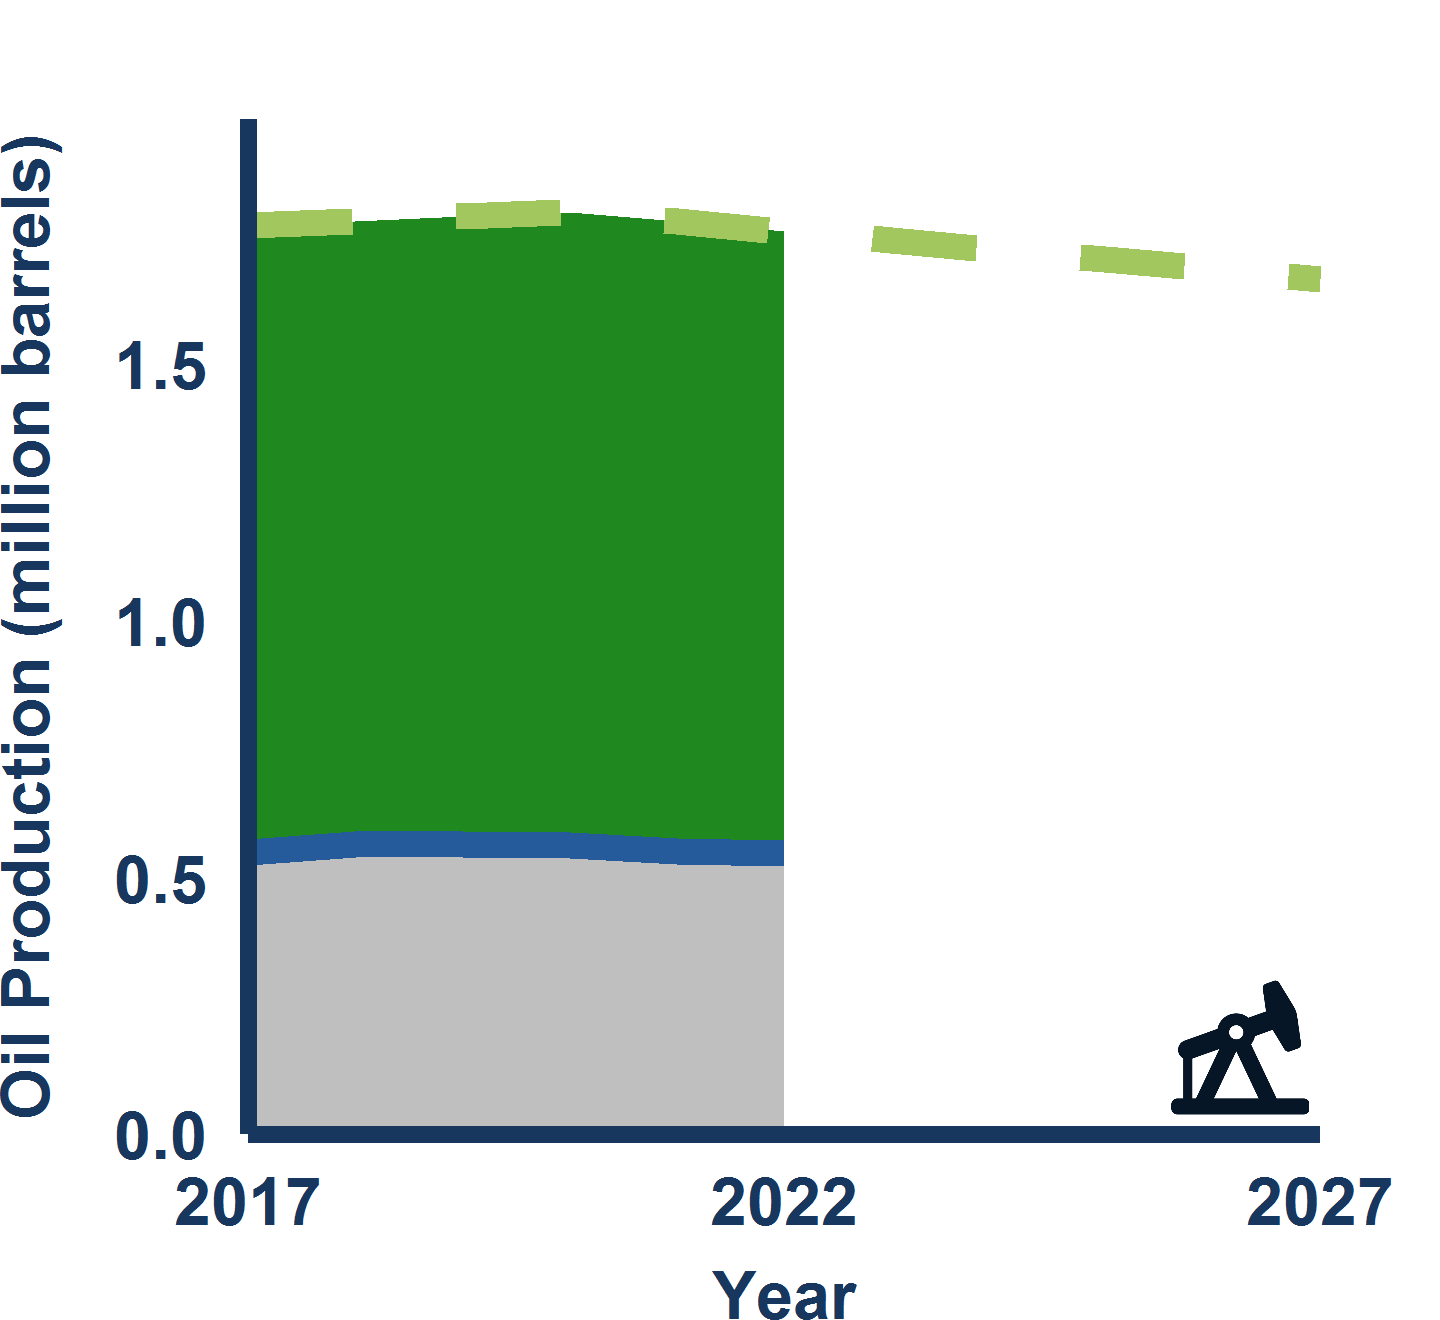
\includegraphics[trim = {0 0cm 0 0},width=1\linewidth]{Figures/Fig29}
		
	\end{minipage}		
	
	
	\begin{center}
		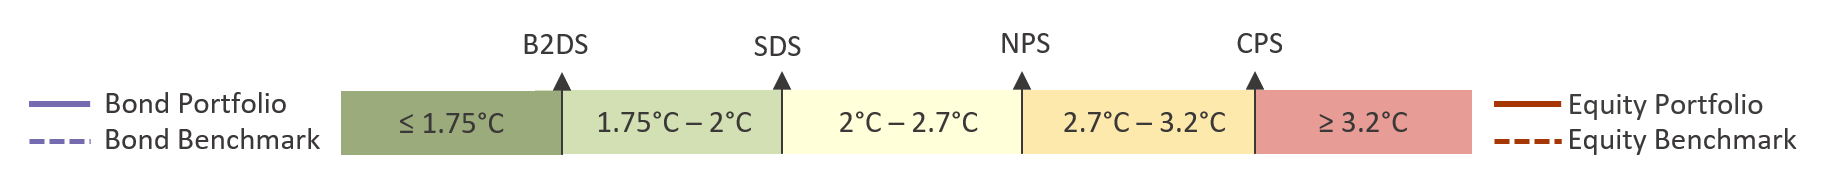
\includegraphics[trim = {0 0cm 0 0},width=.8\linewidth]{ReportGraphics/246Legend.png}
	\end{center}
	
	\PageFooterThird
	\newpage %EQSpecificE
	\section*{} % OTHER SECTORS % OtherSectorsMaterialS
	\HeaderSingle{EMISSION INTENSITY - CEMENT AND STEEL}
	
		\begin{multicols}{2}
			As mentioned in the introduction to this report, there are a number of sectors for which no zero carbon technology exists or has yet been modeled by IEA 2°C scenarios (not considering partial substitutes, such as wood for cement). This applies in particular to the steel, cement, ship and air transport sectors. These sectors are therefore analyzed here.
			
			For these sectors, decarbonisation efforts will be confined to increasing efficiency in production and use, as well as investment in research and 	development in the next 5-10 years, in order to bring CO\textsubscript{2}-neutral alternatives to market maturity in the medium term. As a result, both the scenarios and the data are relatively imprecise.
			
			The figures presented here are based on external CO\textsubscript{2} intensity estimates, themselves based on a publicly available emission estimation model developed by the 2° Investing Initiative together with the consulting company EY. For shipping, an external CO\textsubscript{2} rating model developed by 	Rightship and the Carbon War Room has been used. Since this model is estimated externally and top-down, it is associated with some uncertainties. The results should therefore be considered as estimates, in contrast to previous analyses in the energy, electricity and automotive sectors. In the following paragraphs, the sectors are considered individually.
			
			After chemicals, steel production is the second largest energy consumer among industrial sectors and the most carbon-intensive sector. The deployment of 	electric arc furnaces is key to reducing emissions (even if this technology remains carbon-emitting). The rate of deployment of this more efficient process is therefore presented in combination with the intensity of CO\textsubscript{2}. If your portfolio is invested in these sectors, the results illustrate the estimated carbon intensity per tonne of steel and cement produced for the equity/bond portfolio as well as the benchmark 2°C. The results are based on the sectoral decarbonization pathways defined by the Science-based Targets Initiative, developed by WWF, WRI and CDP.
			
			These results can serve as a starting point for discussions with steel producers on carbon intensity and strategies consistent with a 2°C climate 	objective. The data presented here are unfortunately too imprecise for the implementation of portfolio allocation strategies.
			
			\end{multicols}
		
			\begin{multicols}{2}
					
				\textbf{Cement}
				
				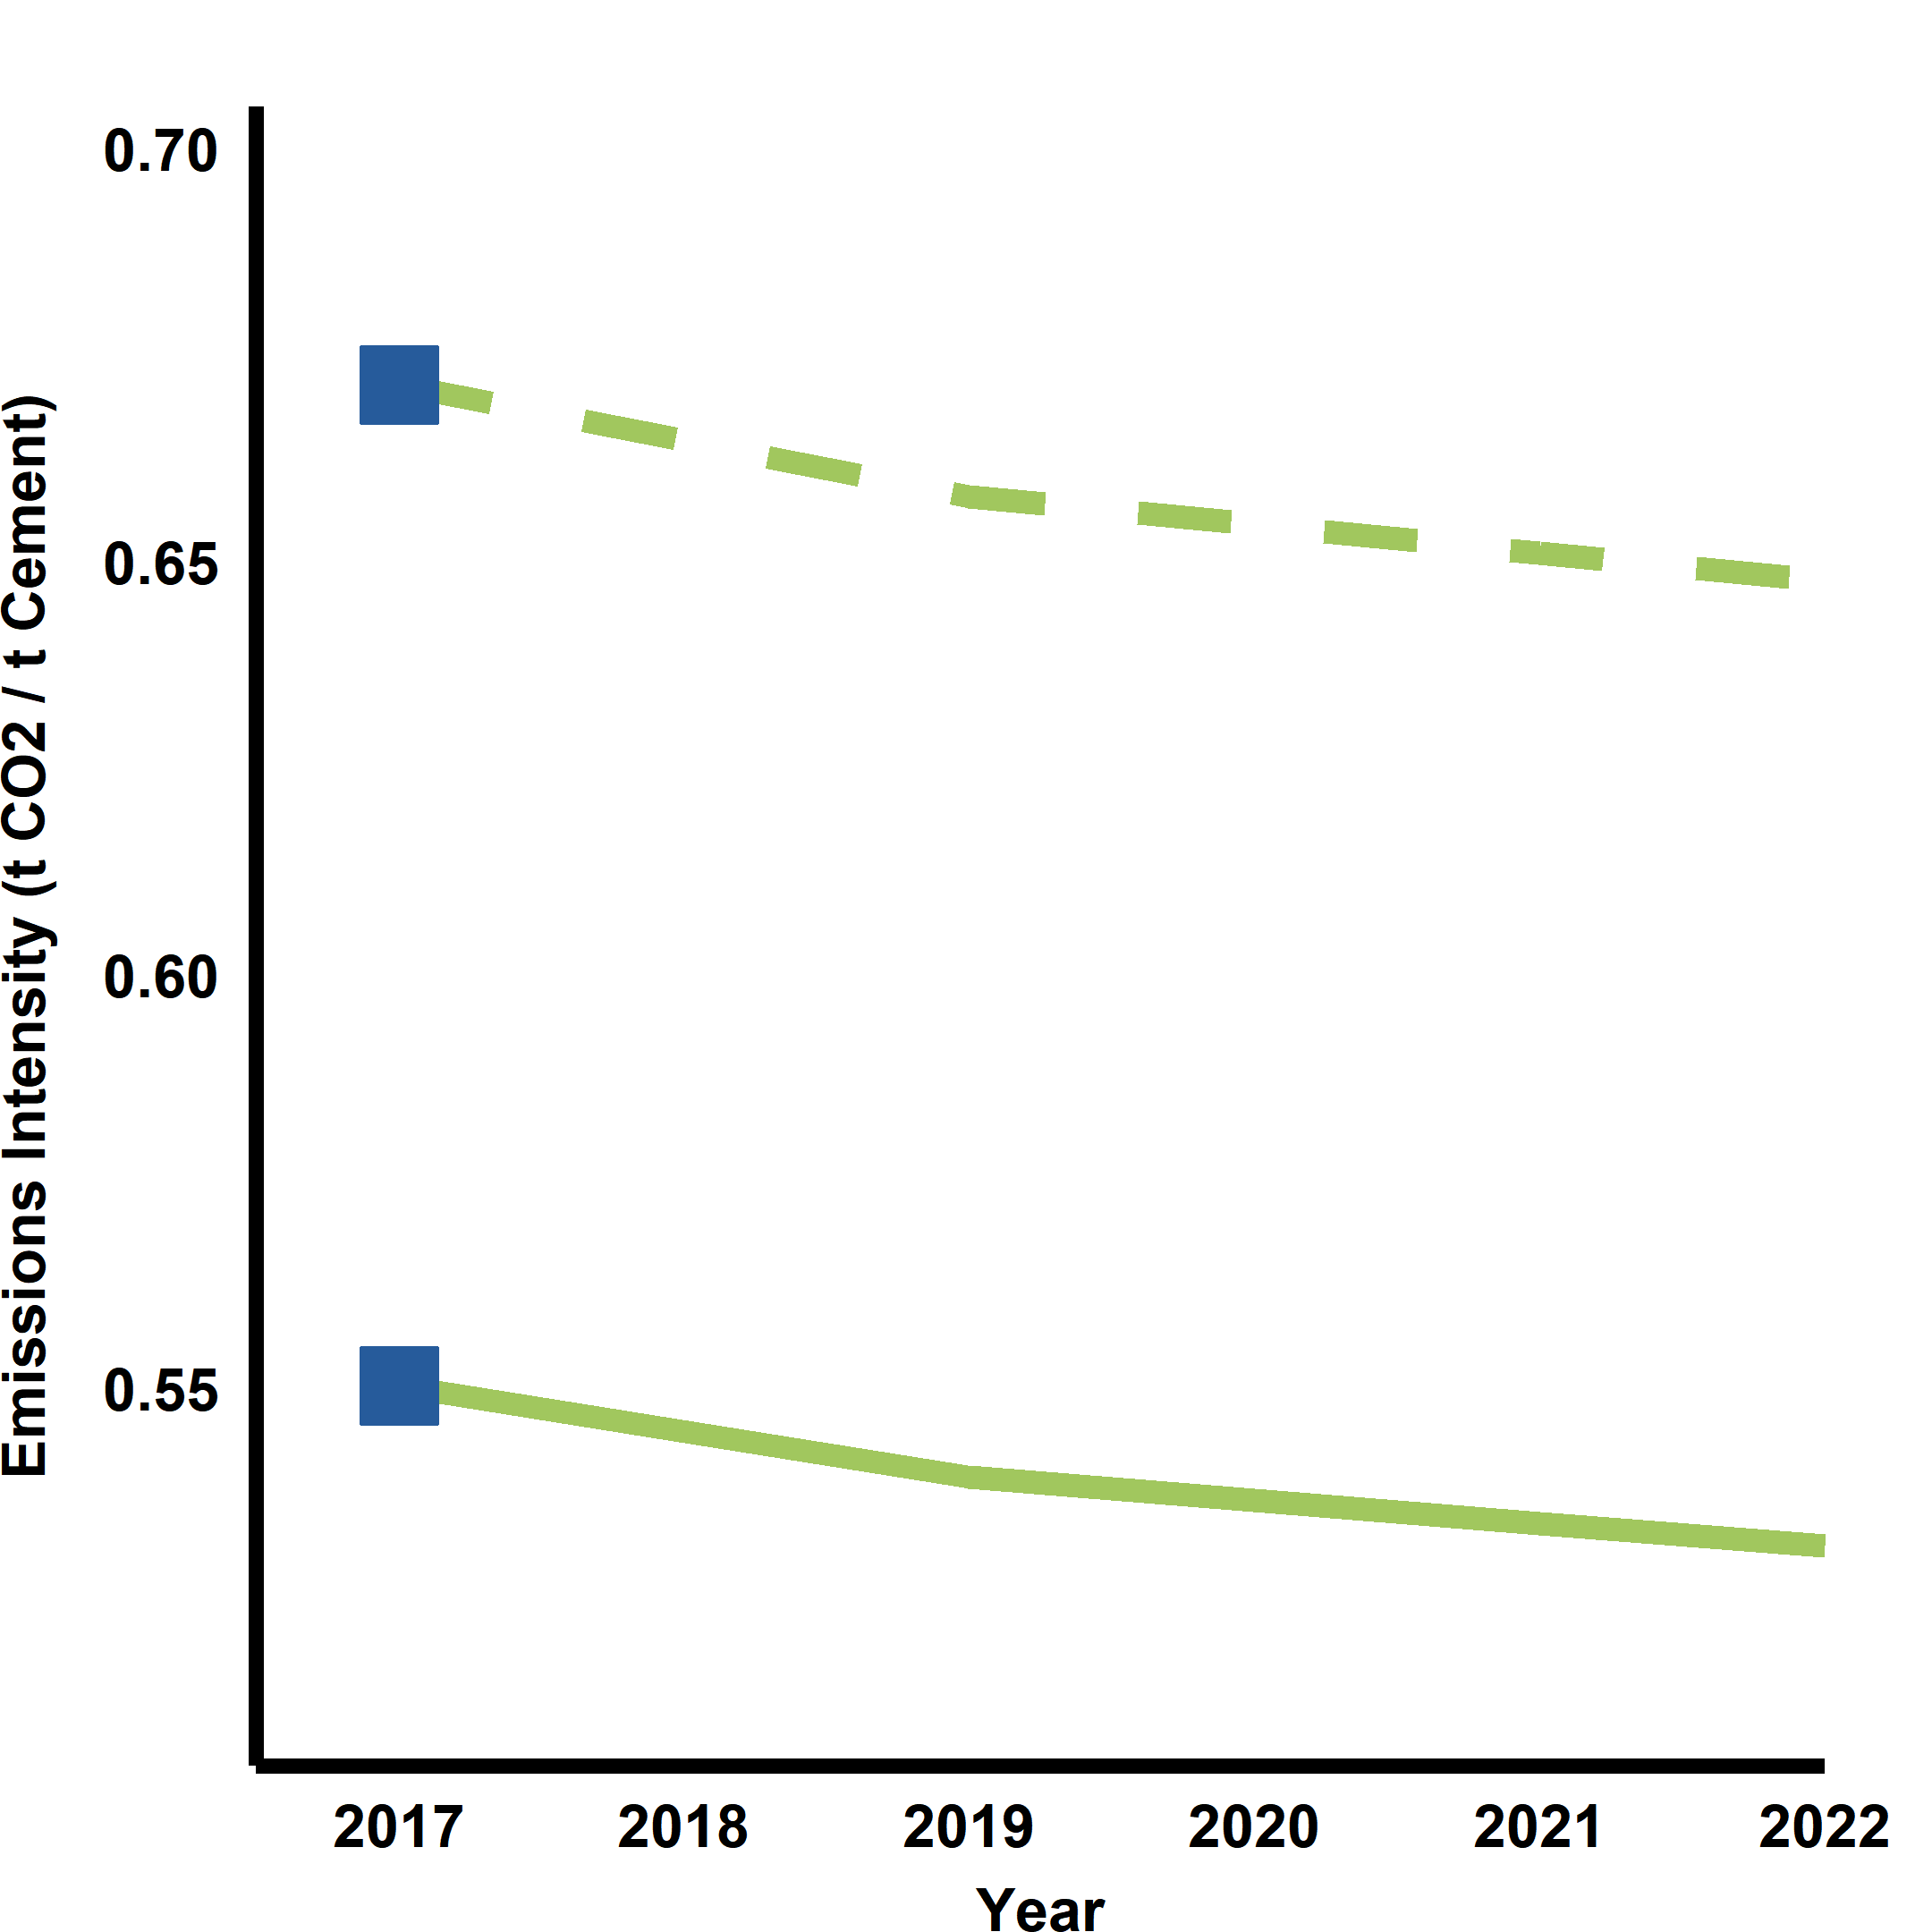
\includegraphics[width=.9\linewidth]{Figures/Fig41}
			
			
				\textbf{Steel}
					
				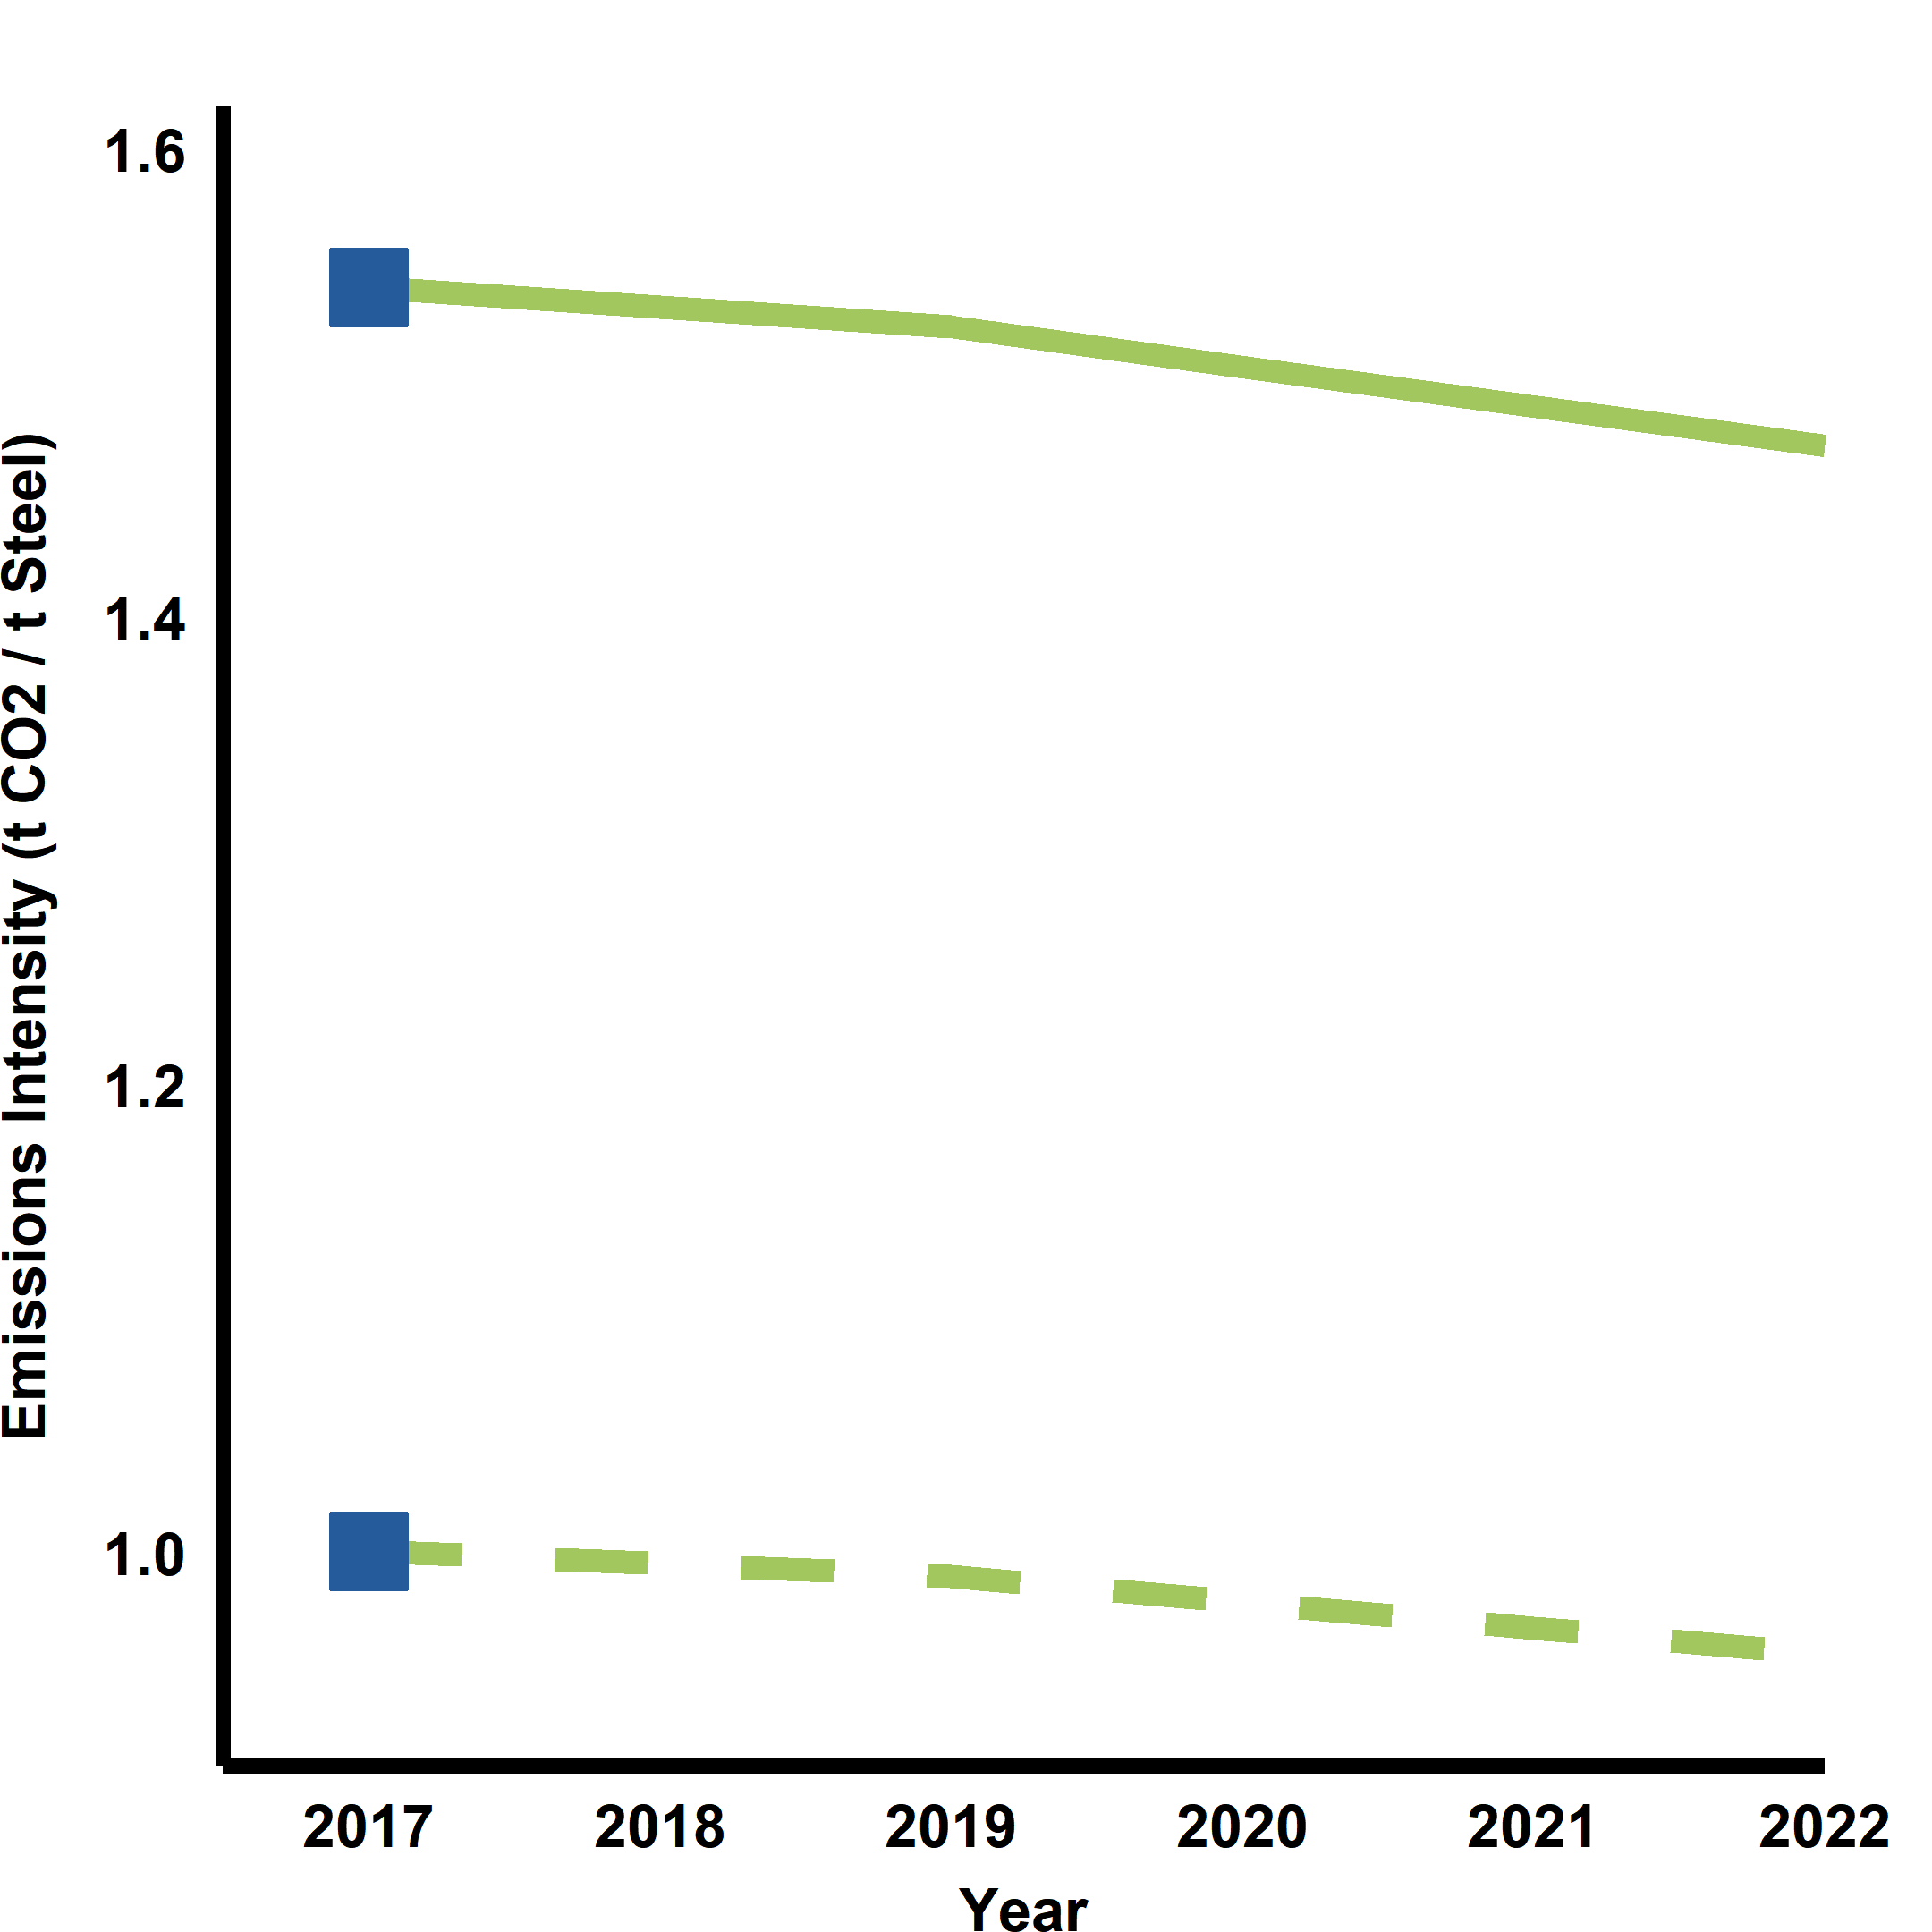
\includegraphics[width=.9\linewidth]{Figures/Fig42}
			
			\end{multicols}
	
	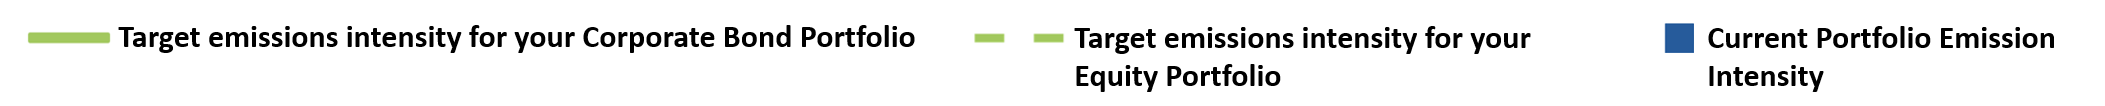
\includegraphics[width=1\linewidth]{ReportGraphics/P16_OtherSectorsLegend_EN}
	
	\textit{\small Source : 2ii based on 2ii/EY 2016, PlantFacts, IEA 2017 and SDA 2015}
	
	\newpage			% OtherSectorsMaterialE
	\section*{} 		% OtherSectorsTransportS 
	\HeaderSingle{EMISSION INTENSITY - AVIATION AND SHIPPING}
		\begin{multicols}{2}
			\textbf{For the shipping and aviation industries, the analysis is focussed on the CO\textsubscript{2} intensity.}
			
			For the aviation sector, we used the Sectoral Decarbonization Approach (SDA) of the Science-Based Target (SBT) project: the curve of the 2°C trajectory 	takes as a starting point the current portfolio situation, the sector average. To convert aircraft fleets into CO\textsubscript{2} emissions, we had to define assumptions on aircraft utilization rates. This introduces a level of uncertainty that does not allow a comparison between airlines. Furthermore, it is important to note that we have only carried out the analysis for the passenger transport shipping; cargo activity is outside the scope.
			
			For the maritime sector, we have not developed a 2°C target. The IEA scenario provides only an indication for the emission trajectory of the sector as a 	whole. However, given the differences between uses (oil tanker, cargo, etc.), it did not make much sense to compare the companies to a global target. So we preferred to apply another method, well established in the market, that only compares companies and portfolios among themselves. This is categorization by Carbon Efficiency Level, developed by Carbon War Room and Rightship. Each vessel is rated from A to G, where A is the best rating. The ranking is dynamically calculated to account for annual improvements in efficiency and variations in the mean, so that "A" ships always represent the top 10\% (measured in terms of CO\textsubscript{2} intensity).
			
			If your portfolio is invested in passenger air transportation, the following charts show the carbon intensity, standardized per kilometer for your stocks 	and bonds. For passenger air transport, the following charts show the carbon intensity, standardized per kilometre for your share portfolio and bonds. If your portfolio is invested in shipping, the charts show the exposure by Carbon Efficiency Rating (A-G) for portfolios and comparison to the average.
			
		\end{multicols}
	
		\begin{multicols}{2}
		
			\textbf{Aviation}
			
			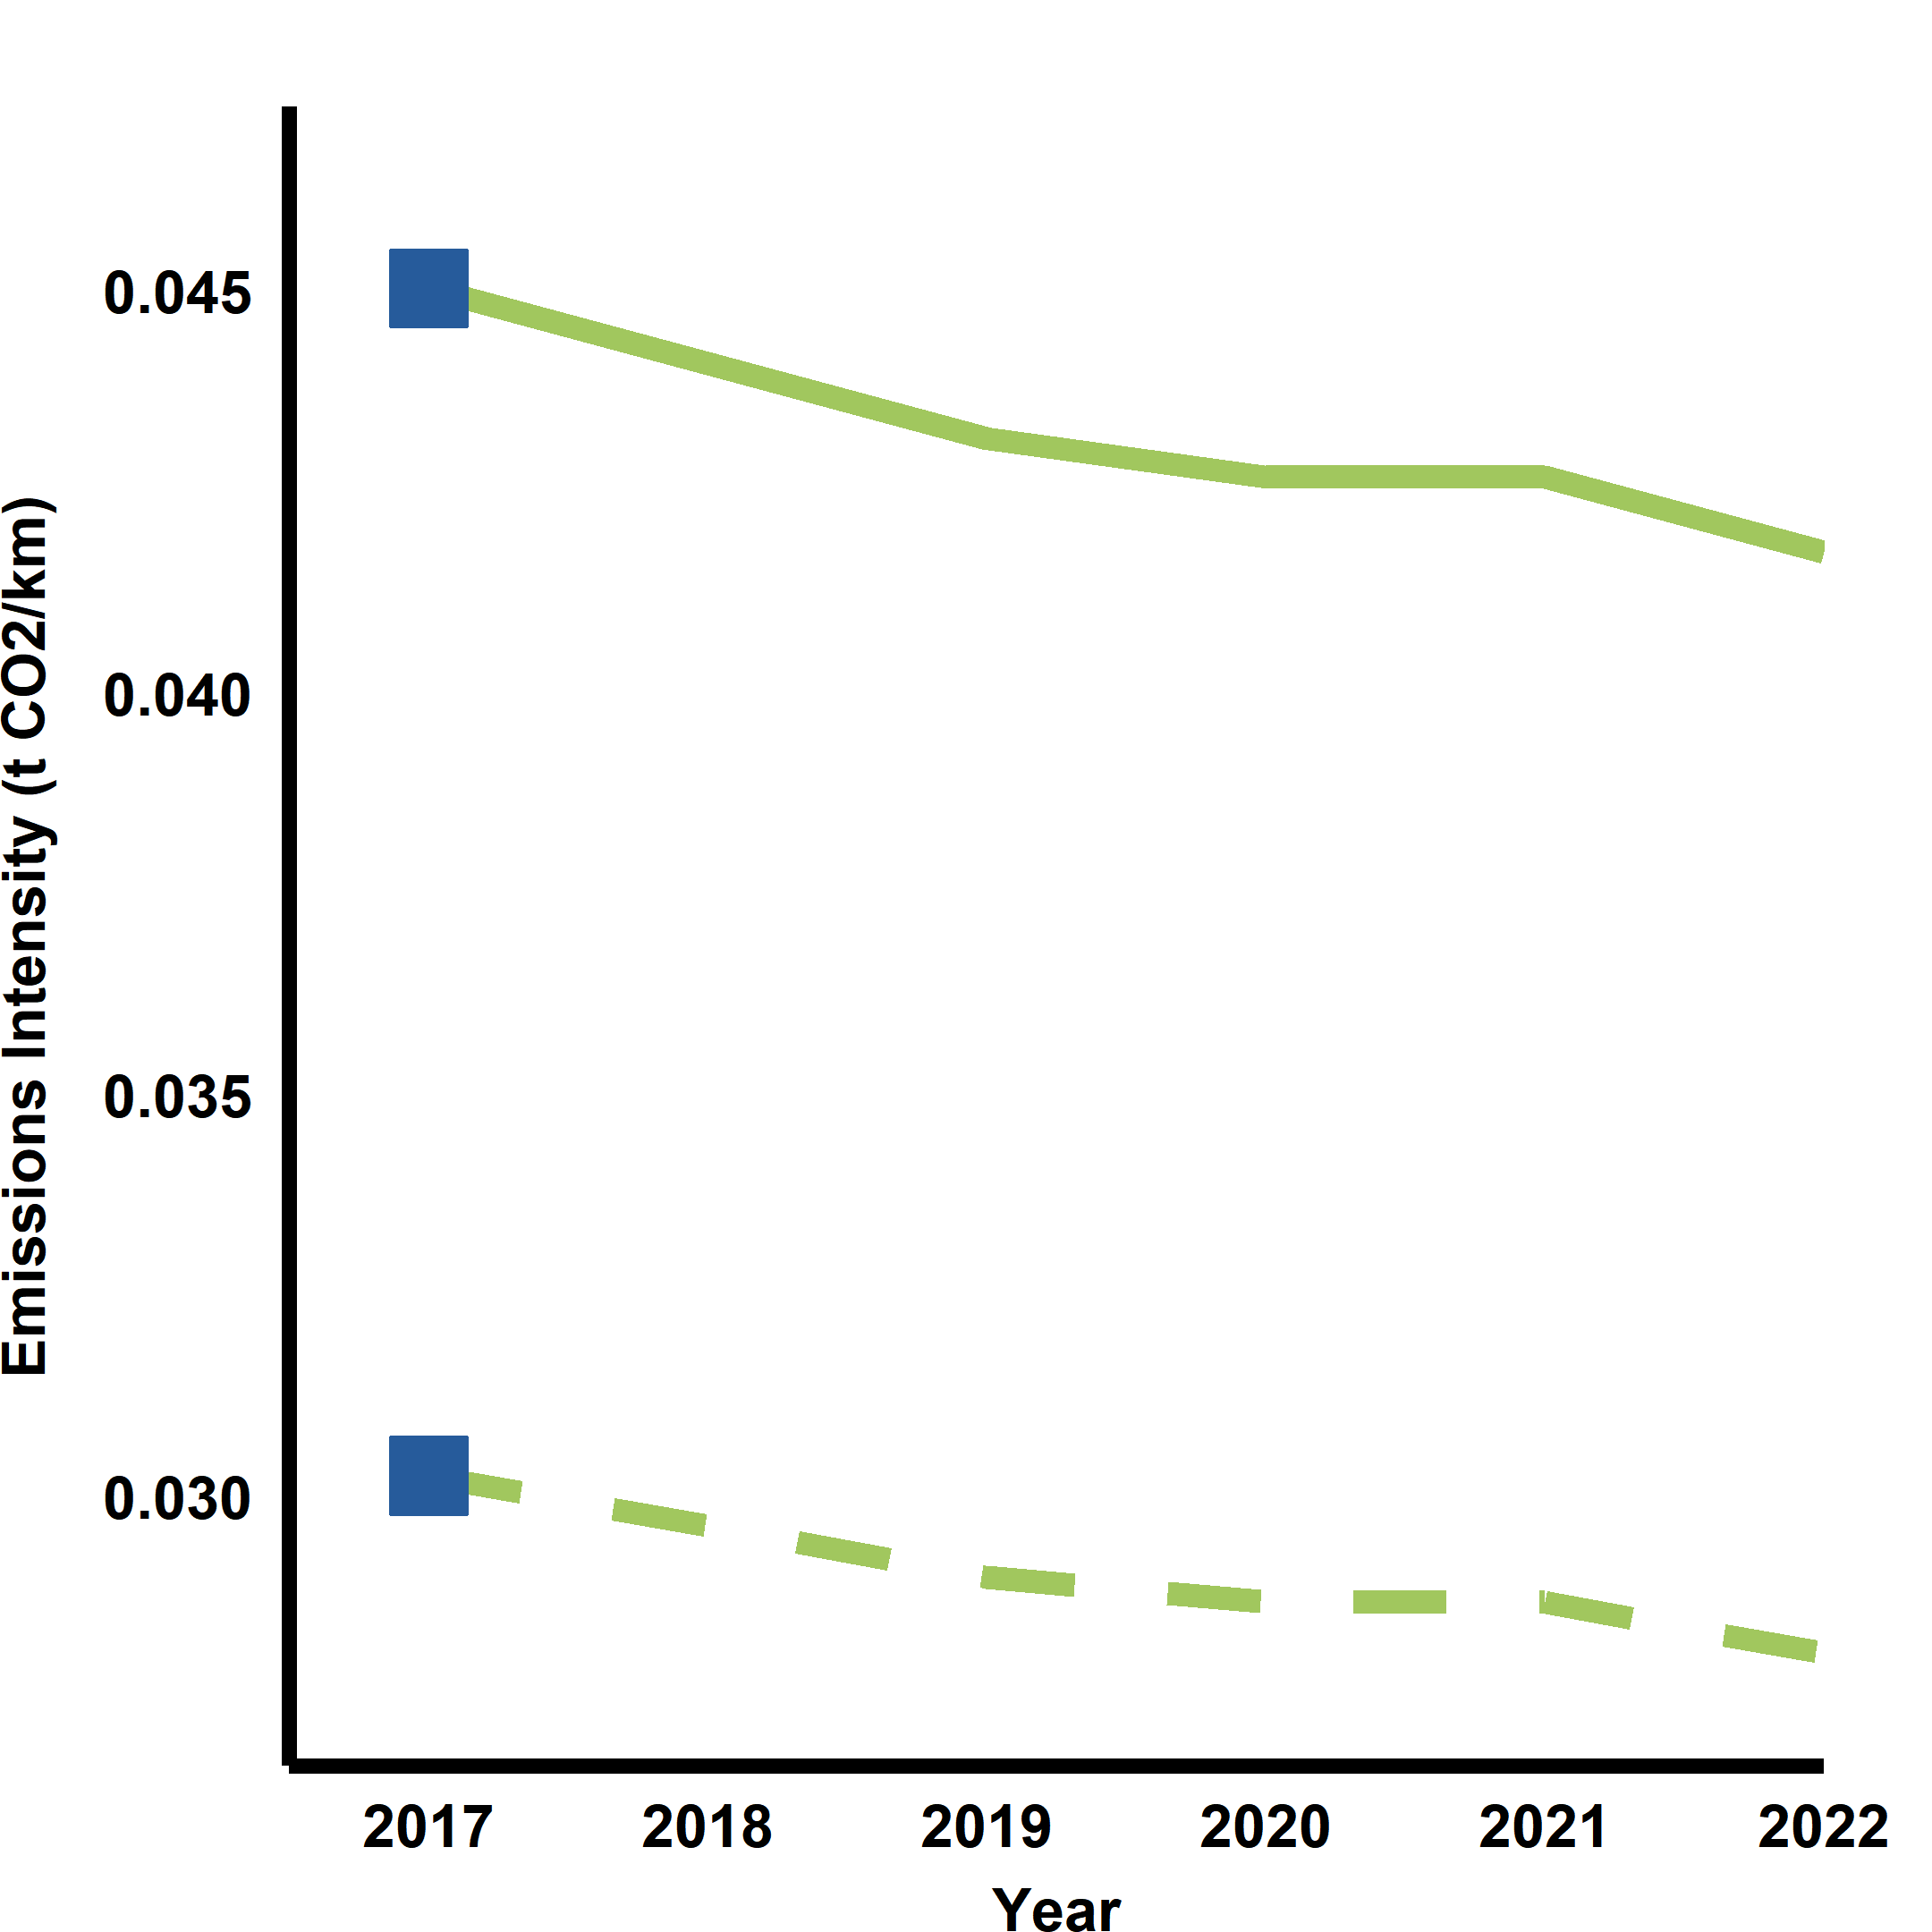
\includegraphics[width=.9\linewidth]{Figures/Fig43}

			\textbf{Shipping}
			
			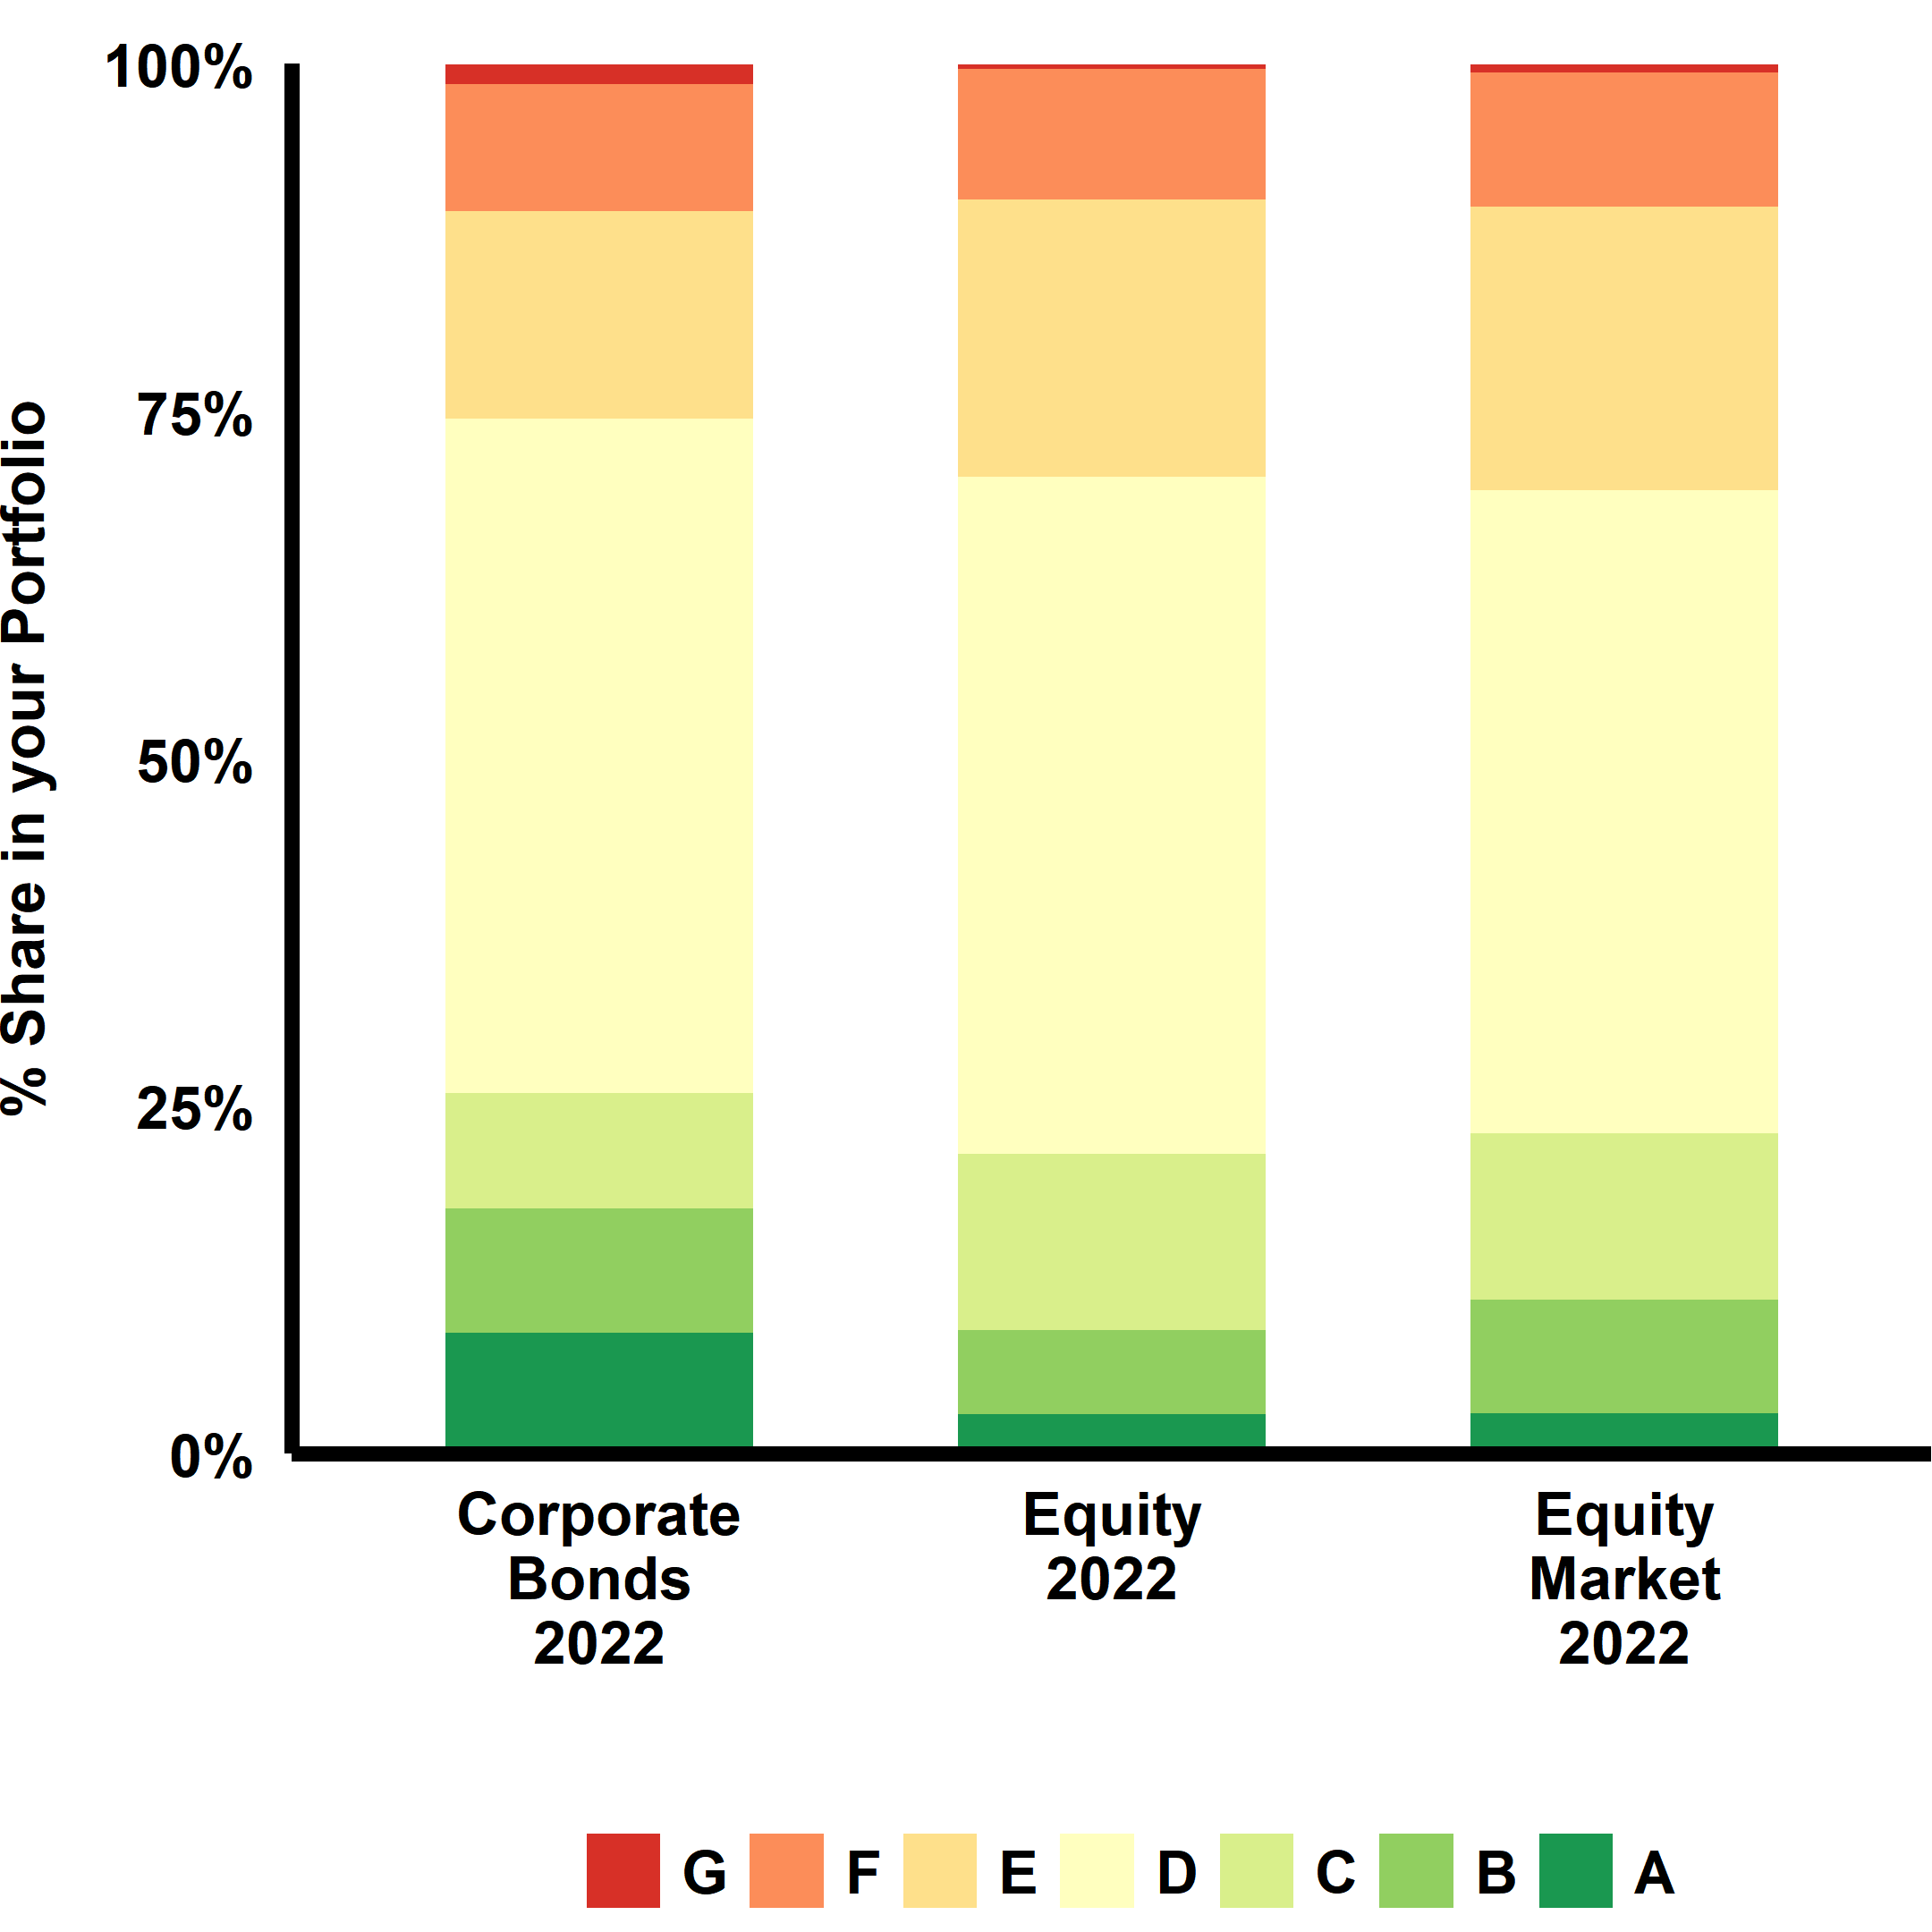
\includegraphics[width=.9\linewidth]{Figures/Fig44}
			
		\end{multicols}
	
	
	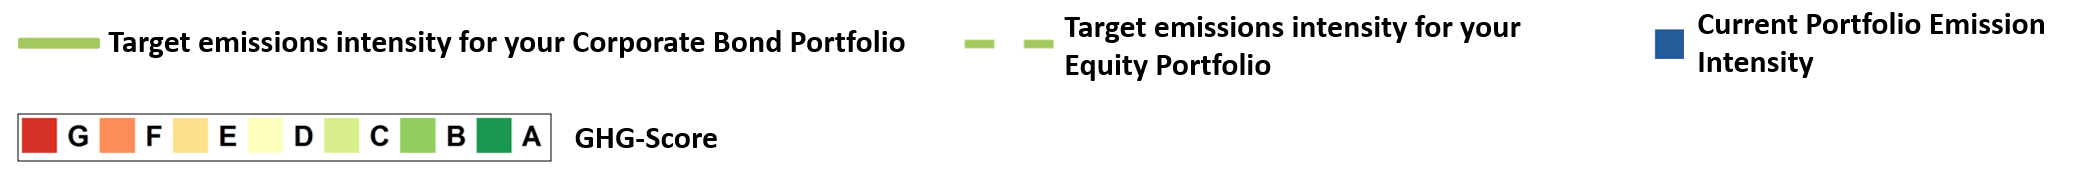
\includegraphics[width=1\linewidth]{ReportGraphics/P17_OtherSectorsLegend_EN}
	
	\textit{\small Source: 2ii based on EY 2016, FlightAscend, and Rightship, Carbon War Room}
	
	\newpage 		% OtherSectorsTransportE
	
	\section*{} 		% FundCheckS 
	\HeaderSingle{FUNDS OVERVIEW}
	
		\begin{multicols}{2}
	This page shows the results for up to the 20 largest funds in your portfolio. The color code indicates which technologies and for which funds the exposure is more (green) or less (red) aligned with the "benchmark" 2°C. The shading signals the distance to the 2°C benchmark (from bright red or green = close to the benchmark to dark red or green = far from the benchmark). The gray bars indicate that the portfolio is not invested in this sector.
\end{multicols}

		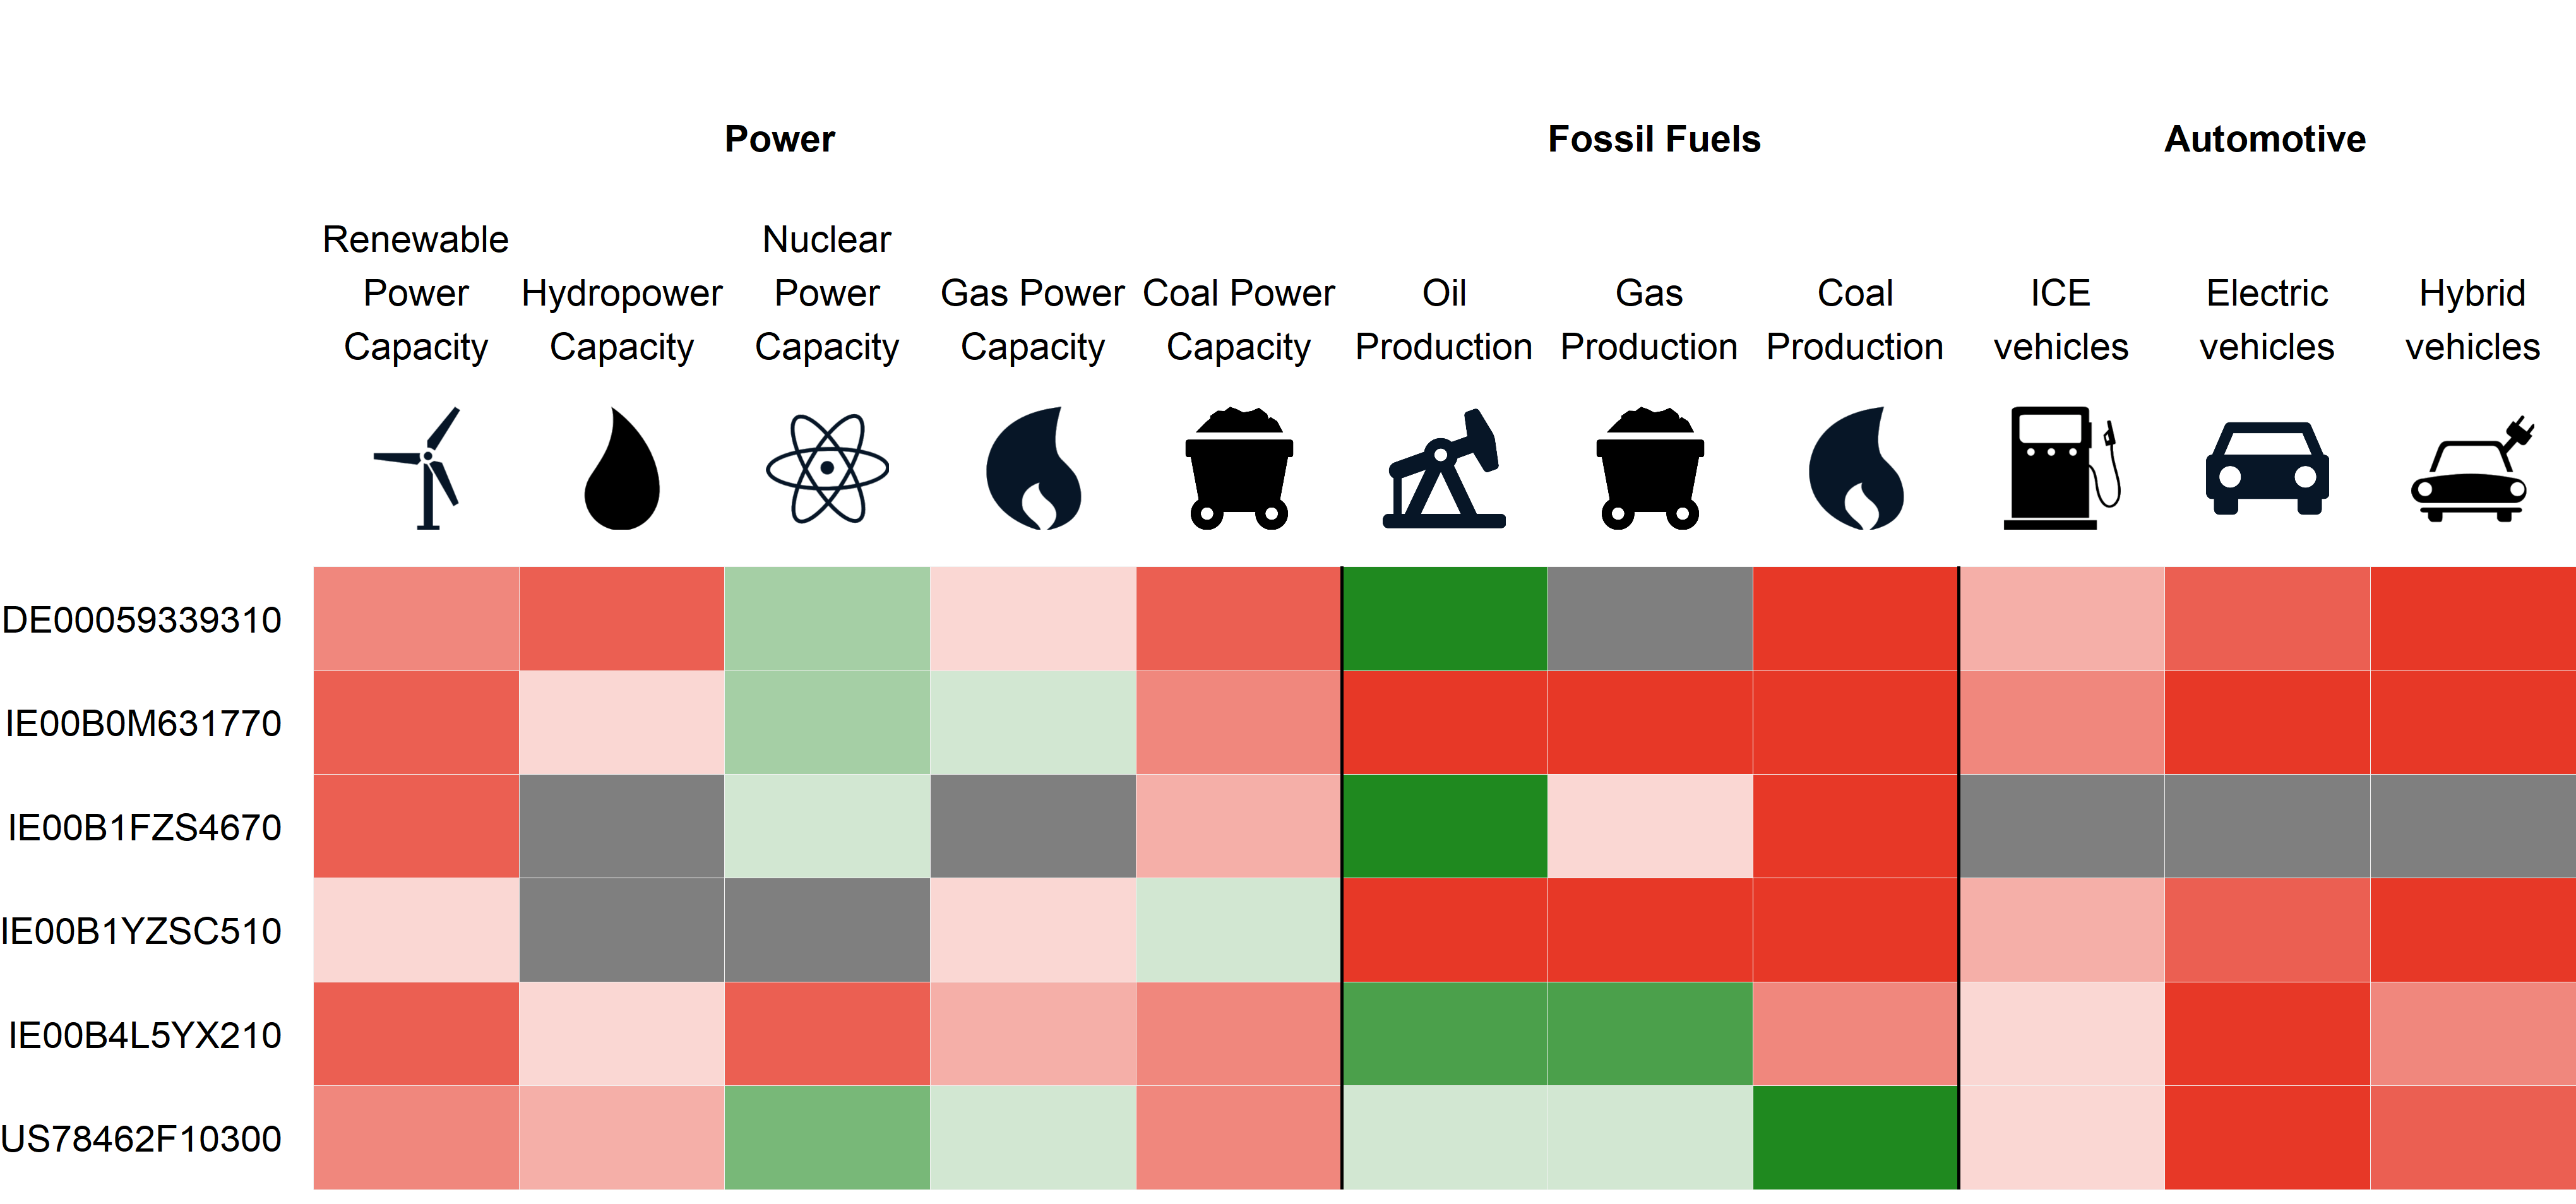
\includegraphics[trim={0 0cm 0 0cm},clip,width=1\linewidth]{Figures/Fig45}
	
	\textit{\small Source: 2ii based on GlobalData, WardsAuto / AutoForecastSolutions, and Morningstar, IEA 2016}
	
	\newpage %FundCheckE
\section*{} % 4th SECTION 
\SectionHeadingDouble{SECTION 4:}{THE EXPOSURE OF YOUR PORTFOLIO}{TO 2°C SCENARIOS IN 2023}


\newpage
	\section*{} % CORP BONDS - RANKING  %CBSpecificS
	\HeaderDouble{FUTURE EXPOSURE – 2023}{BONDS}
	
		\begin{multicols}{2}
			\textbf{The figure below shows the estimated alignment of your bond portfolio in 2023 to the benchmark for each technology or fuel in the climate relevant sectors covered in this analysis. }
			
			The results are a function both of the starting point of the exposure (Section 2) and the evolution of the exposure over time (Section 3) based on current revealed investment and production plans for all companies. The results show the relative alignment of your portfolios across asset classes and technologies or fuels. They should be interpreted as follows:
			
			\begin{itemize}
				\item{0\% alignment suggests the portfolio weights the respective technology / fuel identically to the market in 2023 – freezing both the current portfolio exposure and the current revealed production / investment plans of companies within those portfolios.}
				
				\item{Any figure above 0\% suggests that the portfolio ‘exceeds’ the expected market exposure under a 2°C transition. This implies a higher exposure to low-carbon technologies and a lower exposure to high-carbon technologies. Thus, a figure of 10\% for oil production implies an under-weight of oil production relative to the benchmark by 10\%. }
				
			\end{itemize}
			
			The blue circle represents the alignment of your portfolio in that technology as compared to the benchmark. The black dashed line represents the distribution of 50\% of your peers, with the white circle representing the average of all portfolios. The rank to the right compares the alignment your portfolio to your peers that have production in this technology. 
		
		\end{multicols}
		
		\textbf{Exposure of your bond portfolio to the market benchmark and how this ranks against the comparison group}
		
		
		\begin{center}
			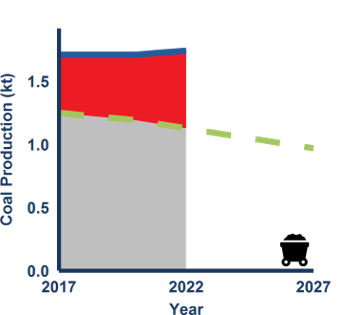
\includegraphics[trim = {0 .8cm 0 0},width=1\linewidth]{Figures/Fig31}
		\end{center}
	
	
	\PageFooterFourth
	\newpage %CBSpecificE
	\section*{} % EQUITY - RANKING %EQSpecificS
	\HeaderDouble{FUTURE EXPOSURE – 2023}{EQUITY}
	
	\begin{multicols}{2}
		\textbf{The figure below shows the estimated exposure of your equity portfolio in 2023 to the technologies and fuels in the climate relevant sectors covered in this analysis. }
		
		The results are a function both of the starting point of the exposure (Section 2) and the evolution of the exposure over time (Section 3) based on current revealed investment and production plans for all technologies. The results show the relative exposure of your portfolios across asset classes and technologies / fuels. They should be interpreted as follows:
		
		\begin{itemize}
			\item{0\% alignment suggests the portfolio weights the respective technology / fuel identically to the market in 2023 – freezing both the current portfolio exposure and the current revealed production / investment plans of companies within those portfolios.}
			
			\item{Any figure above 0\% suggests that the portfolio ‘exceeds’ the expected market exposure under a 2°C transition. This implies a higher exposure to low-carbon technologies and a lower exposure to high-carbon technologies. Thus, a figure of 10\% for oil production implies an under-weight of oil production relative to the benchmark by 10\%. }
			
		\end{itemize}
	
		The blue circle represents the alignment of your portfolio in that technology as compared to the benchmark. The black dashed line represents the distribution of 50\% of the comparison group, with the white circle representing the average of all portfolios. The rank to the right compares the alignment your portfolio to the comparison group that have production in this technology. 
		
	\end{multicols}
	
	\textbf{Exposure of your equity portfolio to the benchmark and how this ranks against the comparison group}
%	\vspace{-0.8cm}
	
	\begin{center}
		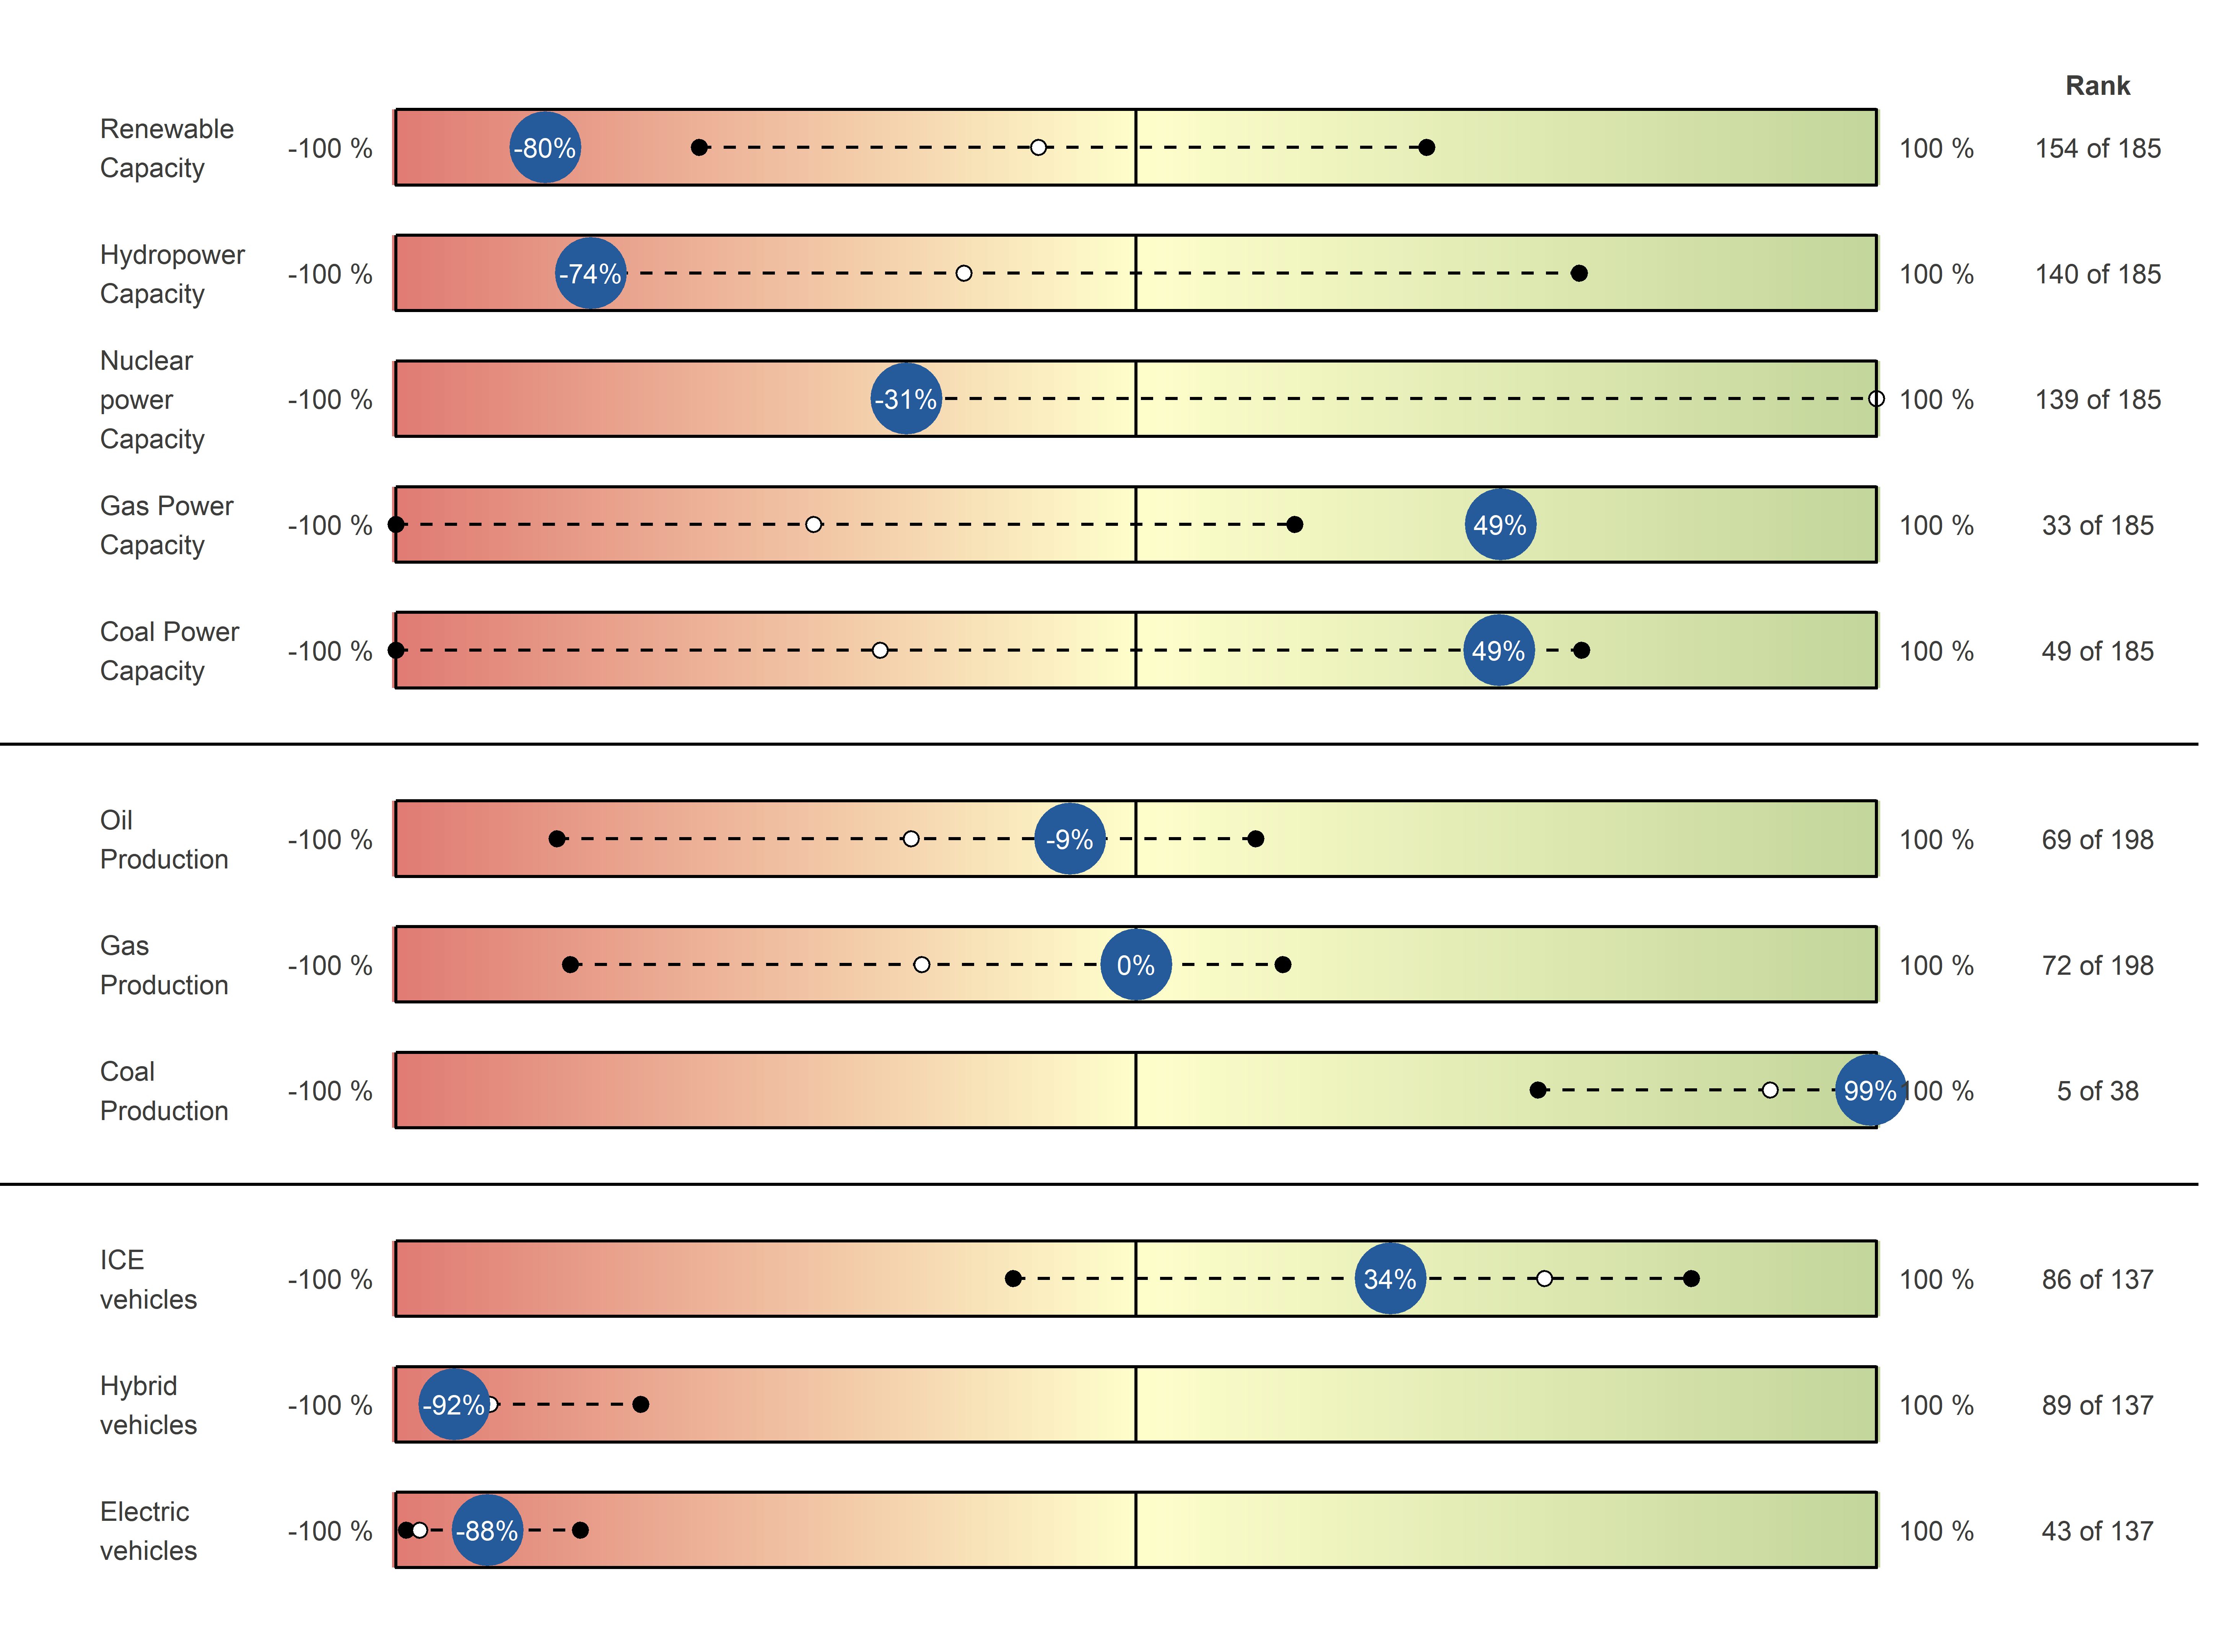
\includegraphics[trim = {0 .8cm 0 0},width=1\linewidth]{Figures/Fig30}
	\end{center}
	
	
	\PageFooterFourth
	\newpage	 %EQSpecificE
\section*{} % 5th COMPANY RESULTS
	\SectionHeading{SECTION 5:}{COMPANY EXPOSURE}
 	\newpage  
	%FossilFuelSectorS

	\section*{} % CONTRIBUTIONS OF SECURITIES TO THE RESULTS
		\HeaderSingle{CONTRIBUTIONS OF SECURITIES TO THE RESULTS}
		
		\begin{multicols}{2}
			Wood Mackenzie (2018) propose that while shifting away from high-carbon fuels towards low carbon is necessary, within the oil and gas industry, shifting away from particular extraction methods is a transitional alternative. This report does not comment on the emissions by extraction type however data is available on this. Companies need to look beyond resource themes and review the variations in upstream emissions intensity to see how companies can reduce their CO\textsubscript{2} footprints. Even assets of the same theme can have significantly different emissions intensity based upon maturity, location and other unique factors.
		\end{multicols}
		%FossilFuelSector_CBS
		\textbf{Resource breakdown of oil production of the largest companies in your bond portfolio}
		
		\begin{center}
						
			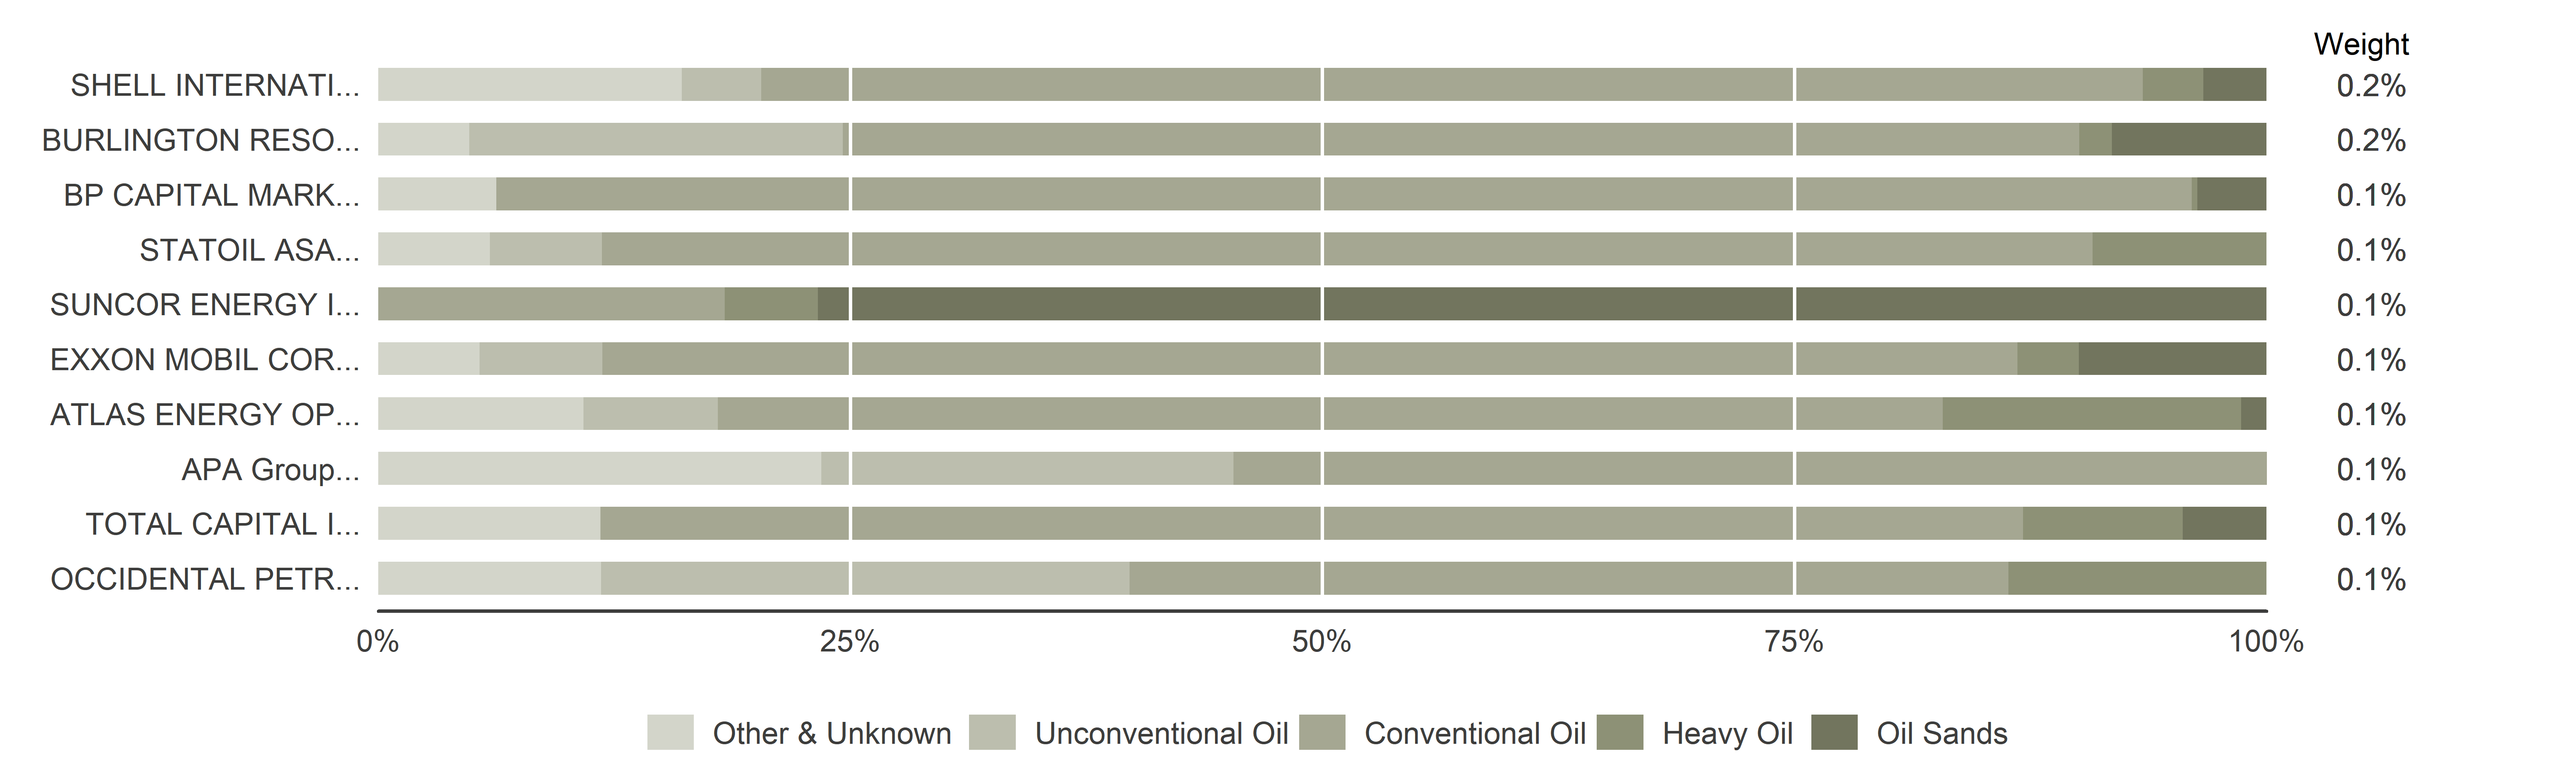
\includegraphics[trim = {0 0cm 0 0},width=1\linewidth]{Figures/Fig38}
		\end{center}
		%FossilFuelSector_CBE
		%FossilFuelSector_EQS
		\textbf{Resource breakdown of oil production of the largest companies in your equity portfolio}

		\begin{center}

			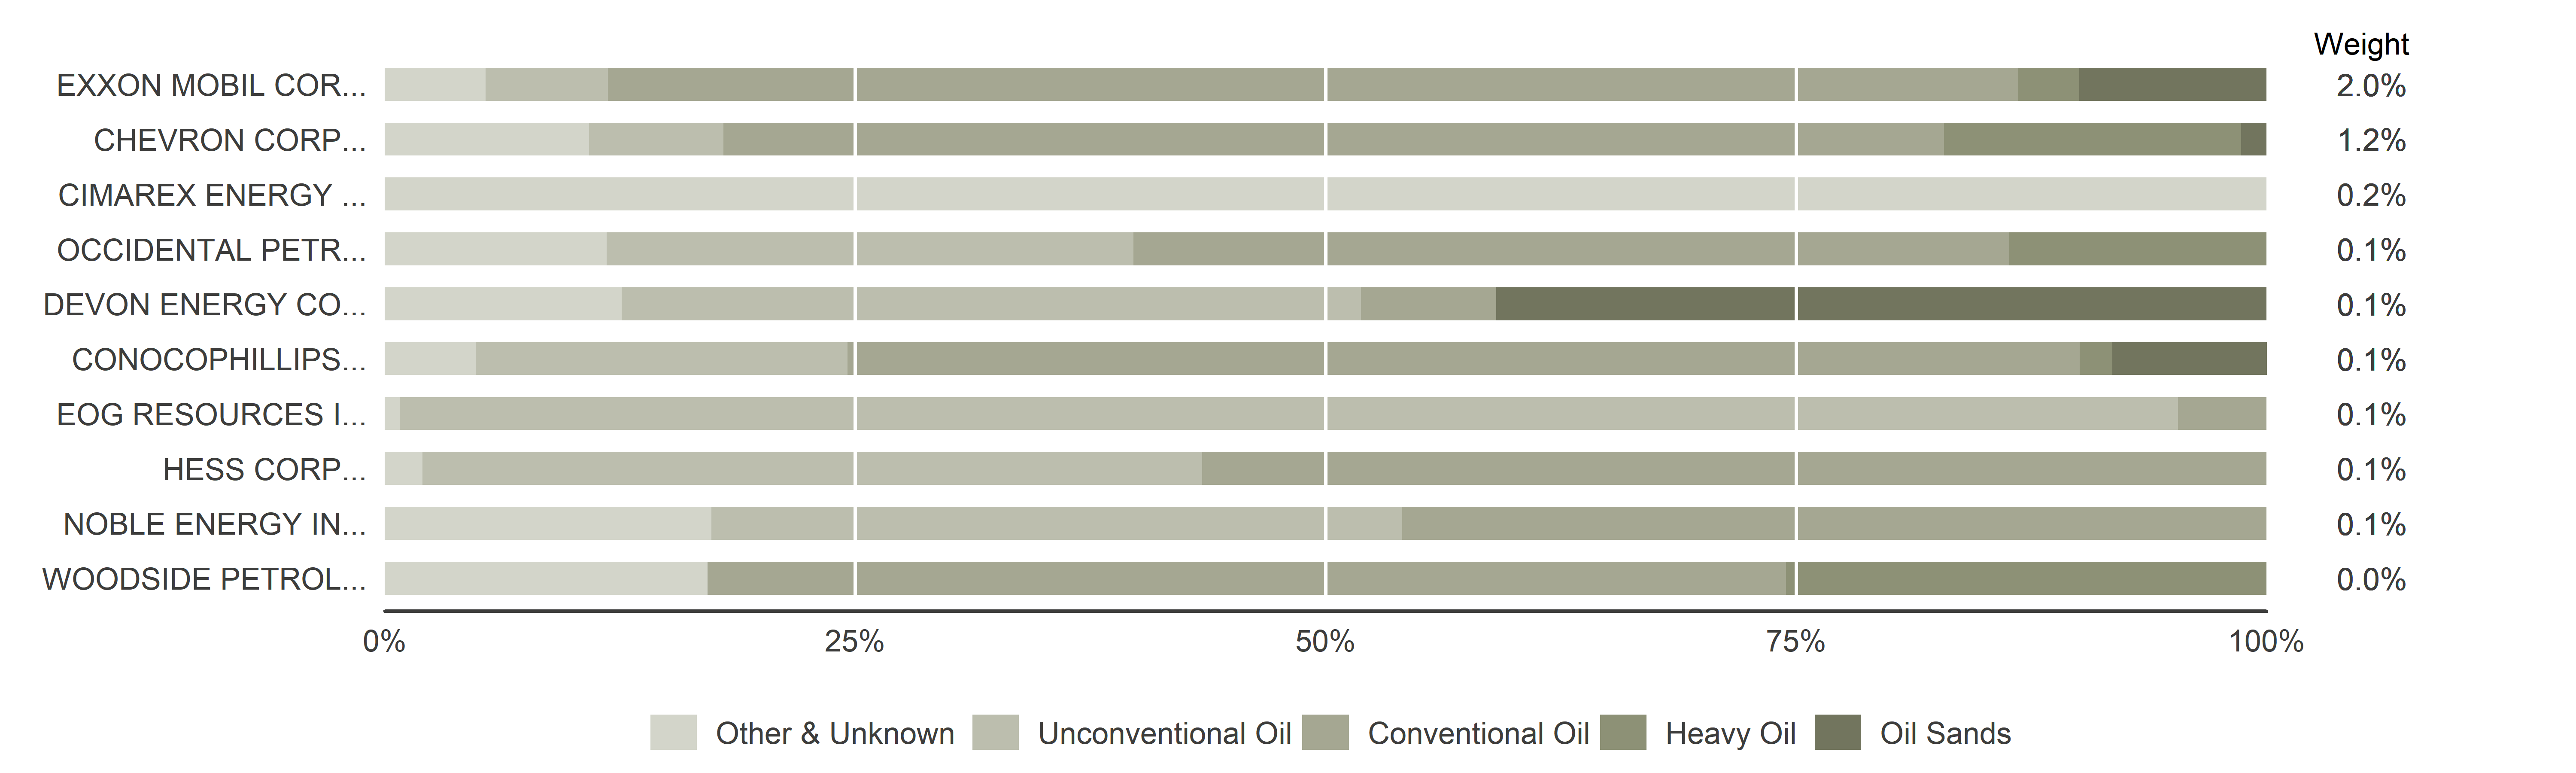
\includegraphics[trim = {0 0cm 0 0},width=1\linewidth]{Figures/Fig39}
		\end{center}
		%FossilFuelSector_EQE

	\PageFooterFifth
	\newpage
	%CarbonBudgetS
	\section*{} % CONTRIBUTIONS OF SECURITIES TO THE RESULTS
		\HeaderSingle{CONTRIBUTIONS OF SECURITIES TO THE RESULTS}
		
		\begin{multicols}{2}
			An alternative assessment of oil companies can be made by comparing the share of oil reserves owned by a company to production that would be outside the 2°C pathway. This is allocated based on the cost curves of oil production, where future production is distributed according to the ‘least-cost principle’.
			On this basis, the share of reserves/future production which is outside the 2°C path is determined. This share is the sum of the future oil production that is above the 2°C price limit, where existing reserves are exhausted. The graph below shows the results for the largest oil and gas companies in your portfolio (across asset classes).
			
			This research was conducted by the Carbon Tracker Initiative. This organisation uses similar asset level databases to compare cost curves to the company production. For more information regarding the methodology, the organisation and further results please refer to this website: https://www.carbontracker.org
			
			
		\end{multicols}
		\textbf{Carbon budget of the largest companies in your equity portfolio}

		\begin{center}

			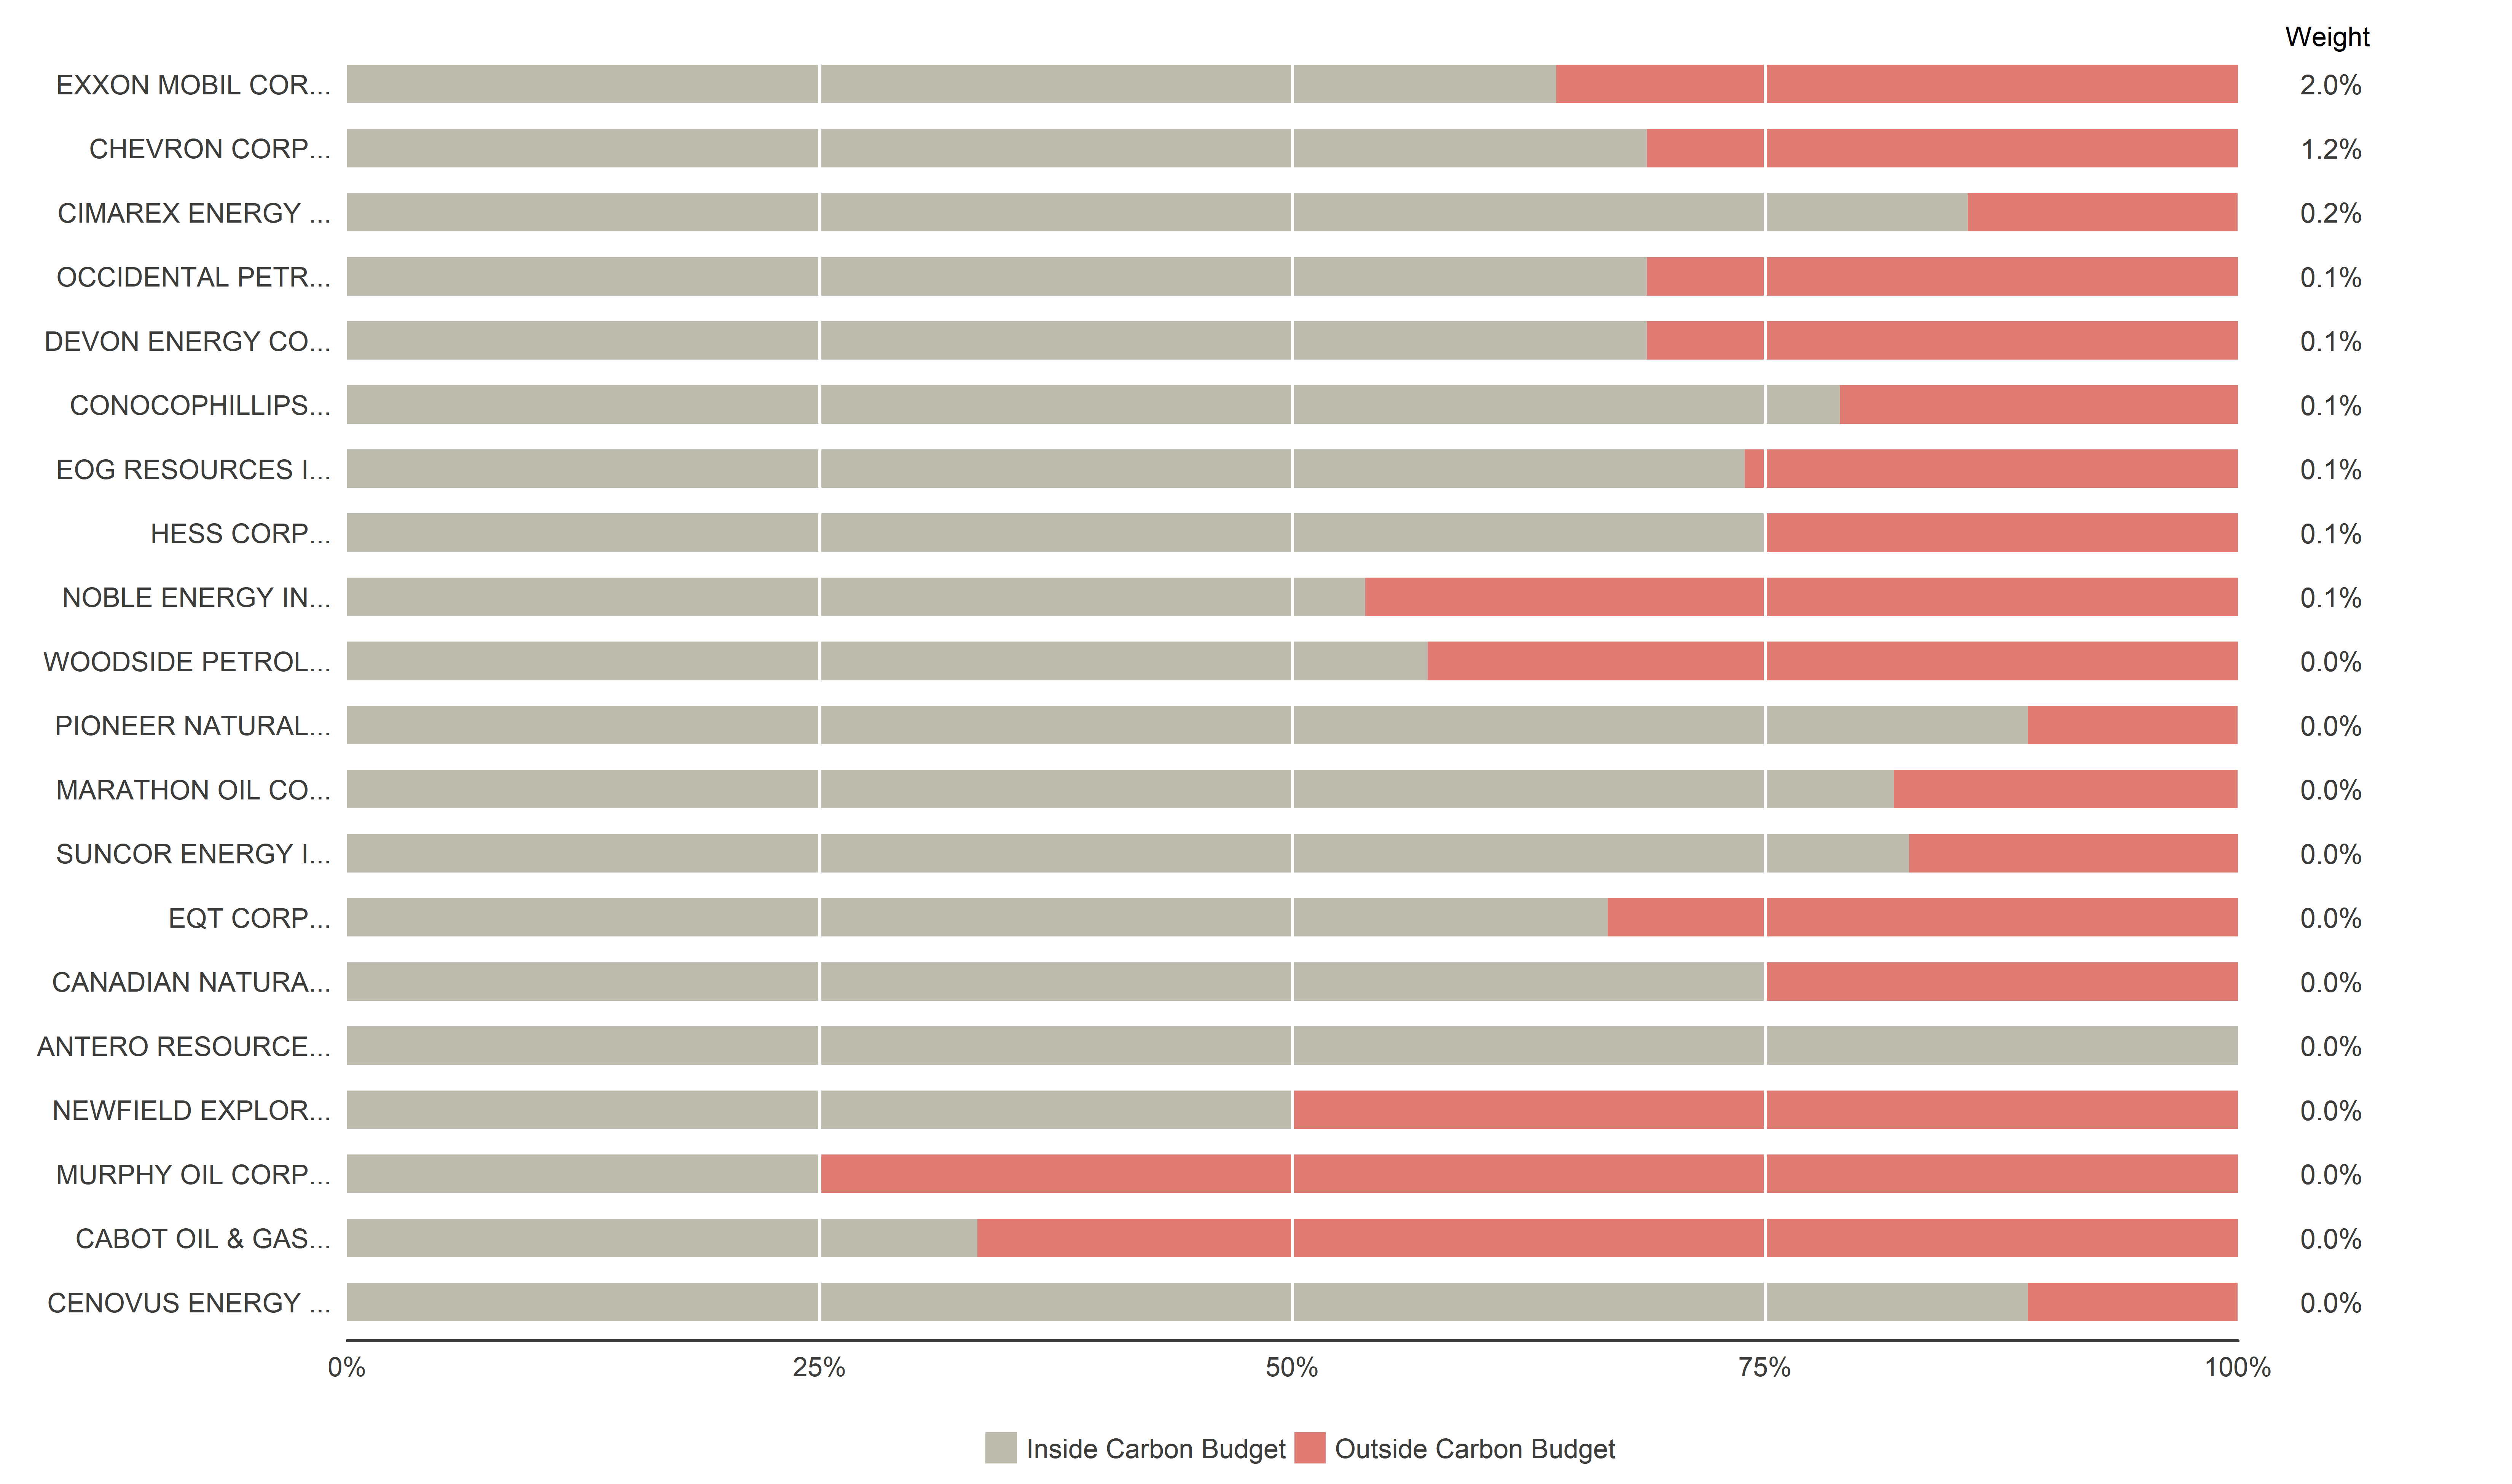
\includegraphics[trim = {0 0cm 0 0},width=1\linewidth]{Figures/Fig40}
		\end{center}

	\PageFooterFifth
	\newpage
	%CarbonBudgetE
	%FossilFuelSectorE
	%PowerSectorS
	\section*{} % CONTRIBUTIONS OF SECURITIES TO THE RESULTS
		\HeaderSingle{CONTRIBUTIONS OF SECURITIES TO THE RESULTS}
	
		\begin{multicols}{2}
			The following chart shows the technology mix of power companies within your portfolio and the stock market. From the accounting principles applied in this test, a portion of capacity from each company has been allocated to your portfolio based on your ownership. The following lists identify the largest contributors by technology identifying both the absolute capacity allocated to your portfolio and what percent of the total capacity of your portfolio this accounts for in 2023. 
			
		
		\end{multicols}
		%PowerSector_CBS
		\textbf{Technology breakdown of power companies within your bond portfolio}
		
		\begin{center}
			
			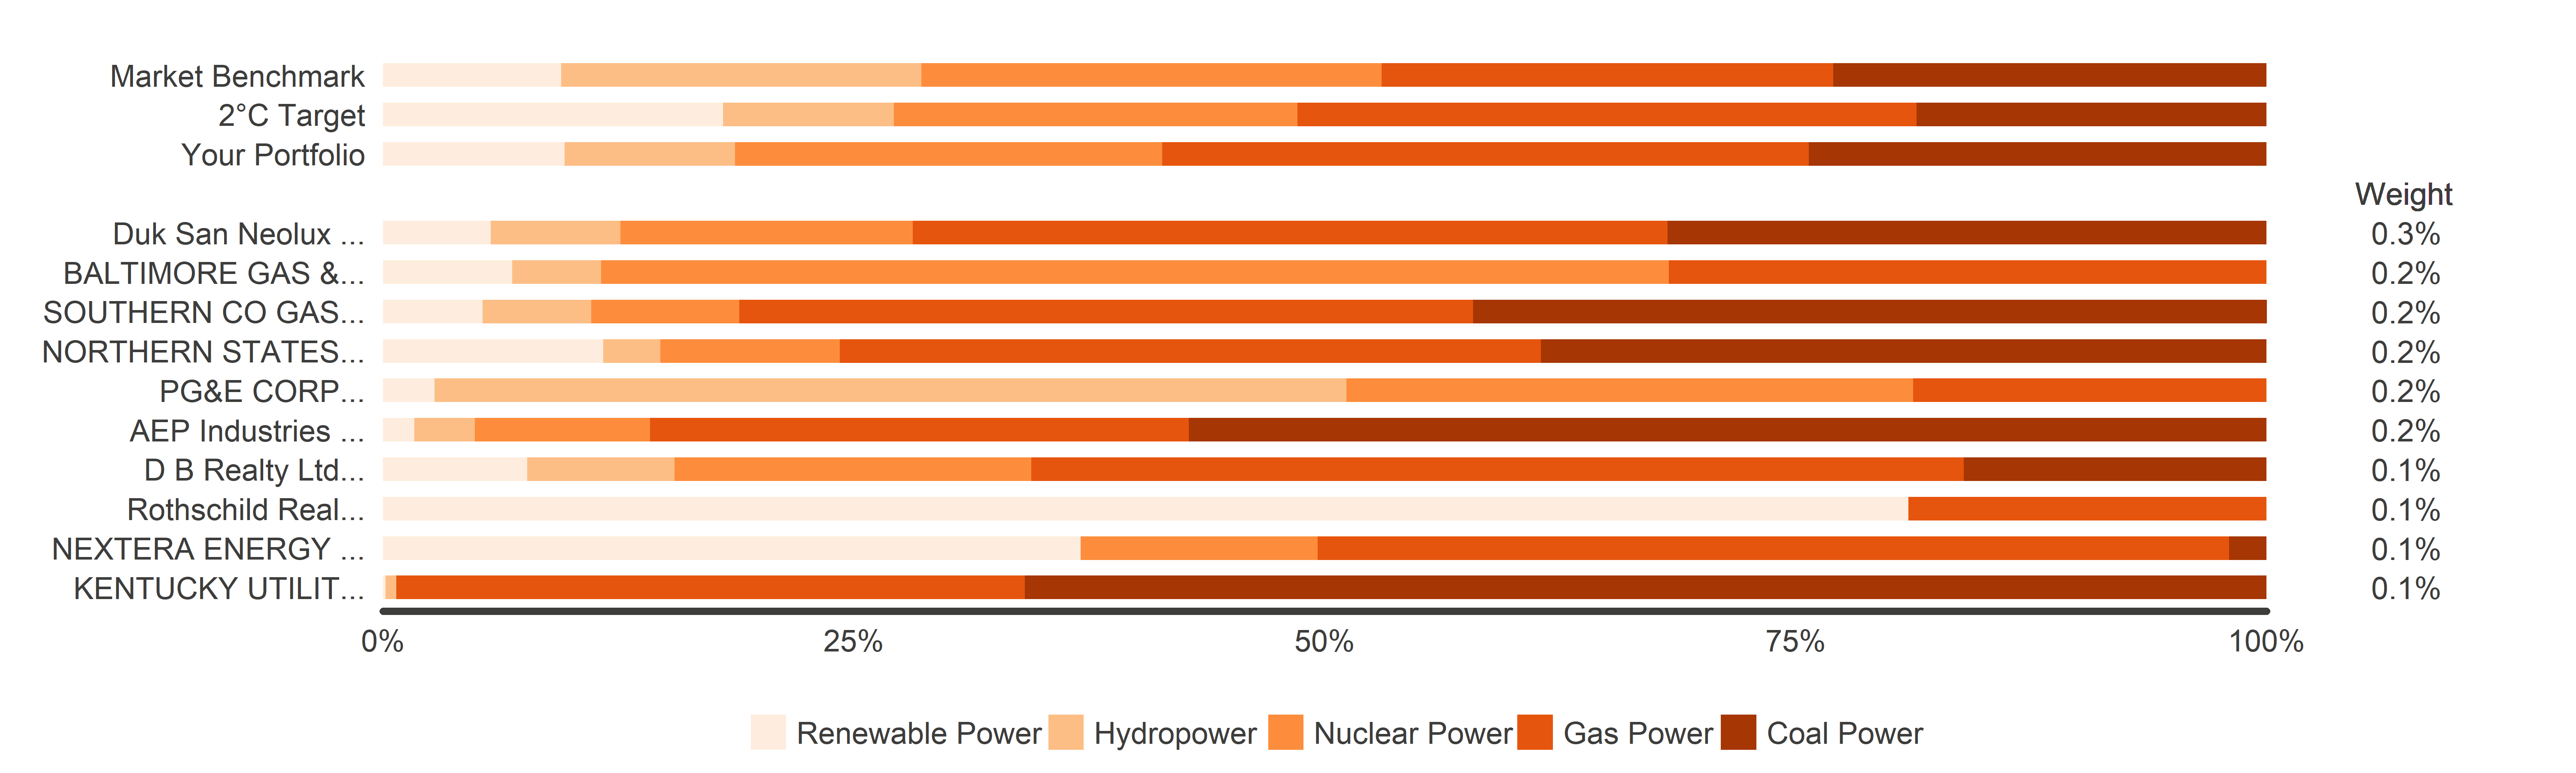
\includegraphics[trim = {0 0cm 0 0},width=1\linewidth]{Figures/Fig32}
		\end{center}
		%PowerSector_CBE
		%PowerSector_EQS
		\textbf{Technology breakdown of power companies within your equity portfolio}

		\begin{center}
			
			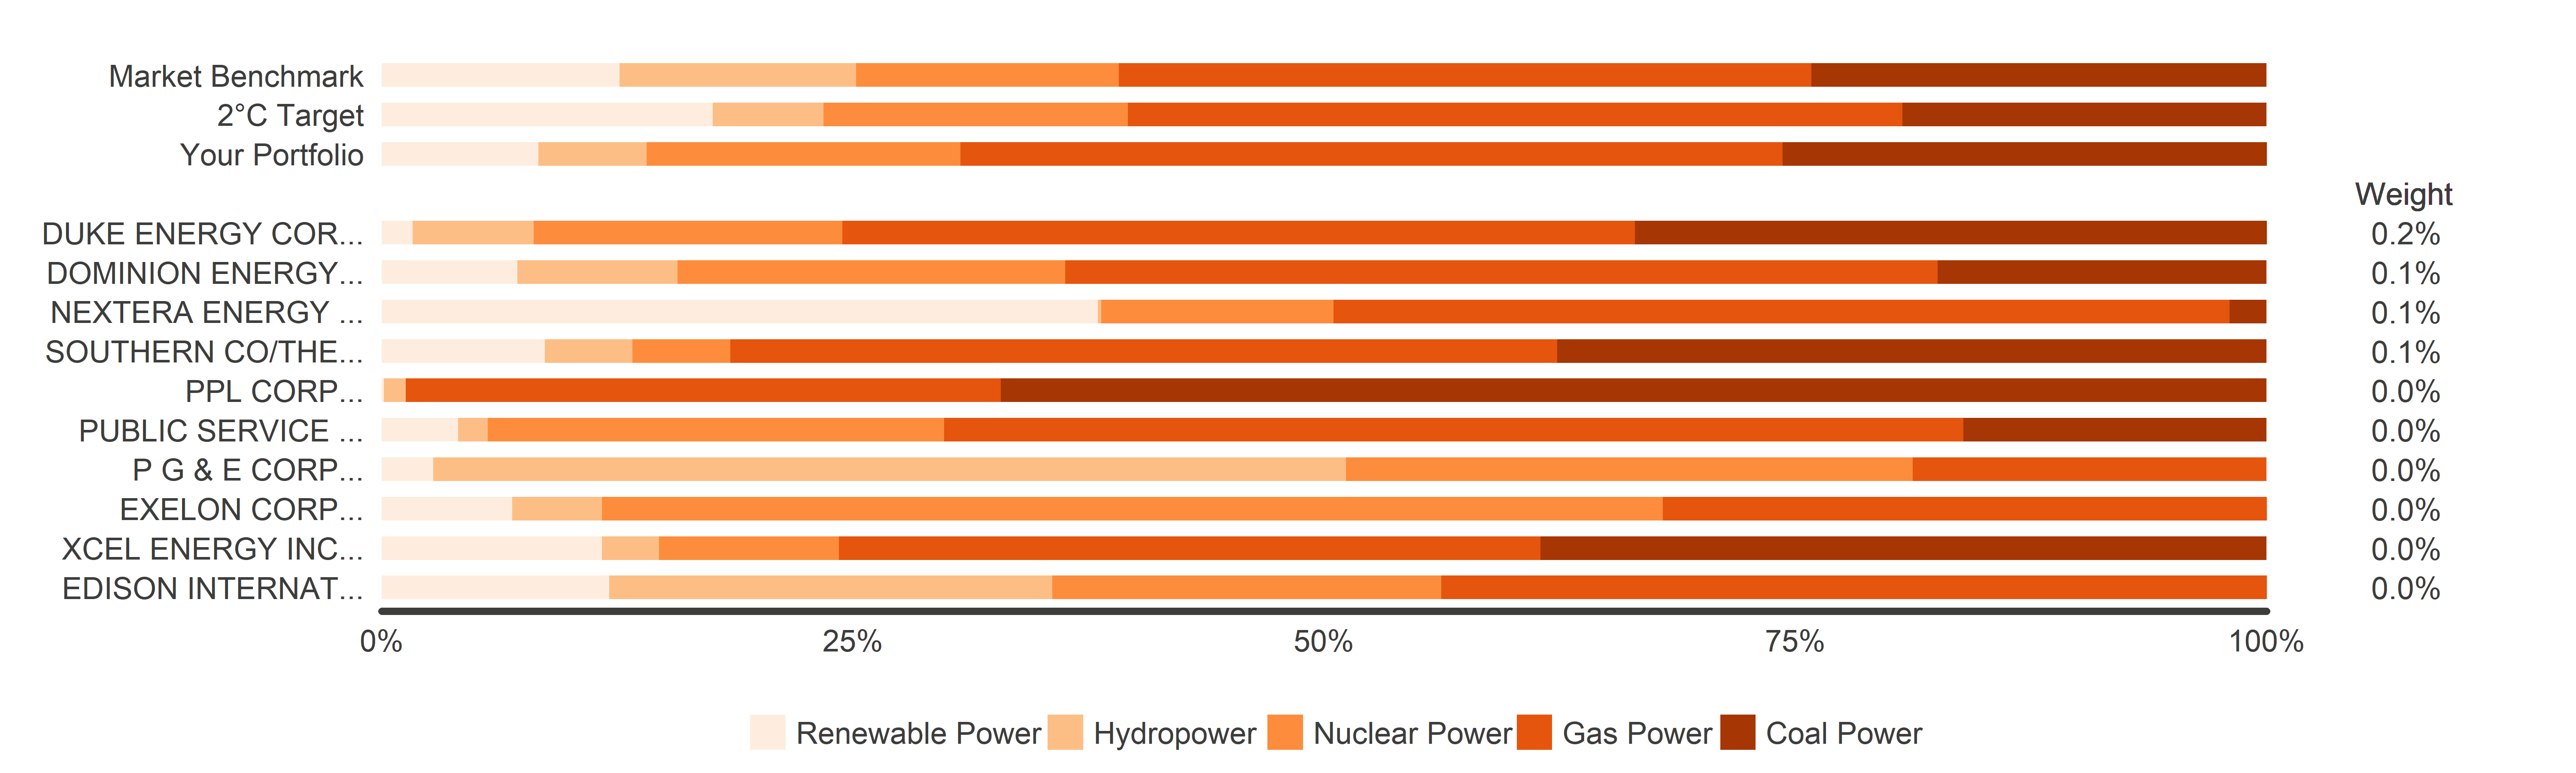
\includegraphics[trim = {0 0cm 0 0},width=1\linewidth]{Figures/Fig33}
		\end{center}		
		%PowerSector_EQE

	\PageFooterFifth
	\newpage
	%PowerSectorE
	%AutoSectorS
	\section*{} % CONTRIBUTIONS OF SECURITIES TO THE RESULTS
		\HeaderSingle{CONTRIBUTIONS OF SECURITIES TO THE RESULTS}

		\begin{multicols}{2}
			The following chart shows the technology mix of Automotive companies within your portfolio and the stock market. From the accounting principles applied in this test, a portion of production from each company has been allocated to your portfolio based on your ownership. The following lists identify the largest contributors by technology identifying both the absolute production allocated to your portfolio and what percent of the total capacity of your portfolio this accounts for in 2023. 
			
			\end{multicols}
			%AutoSector_CBS
			\textbf{Technology breakdown of automotive companies within your bond portfolio}
			
			\begin{center}
			
				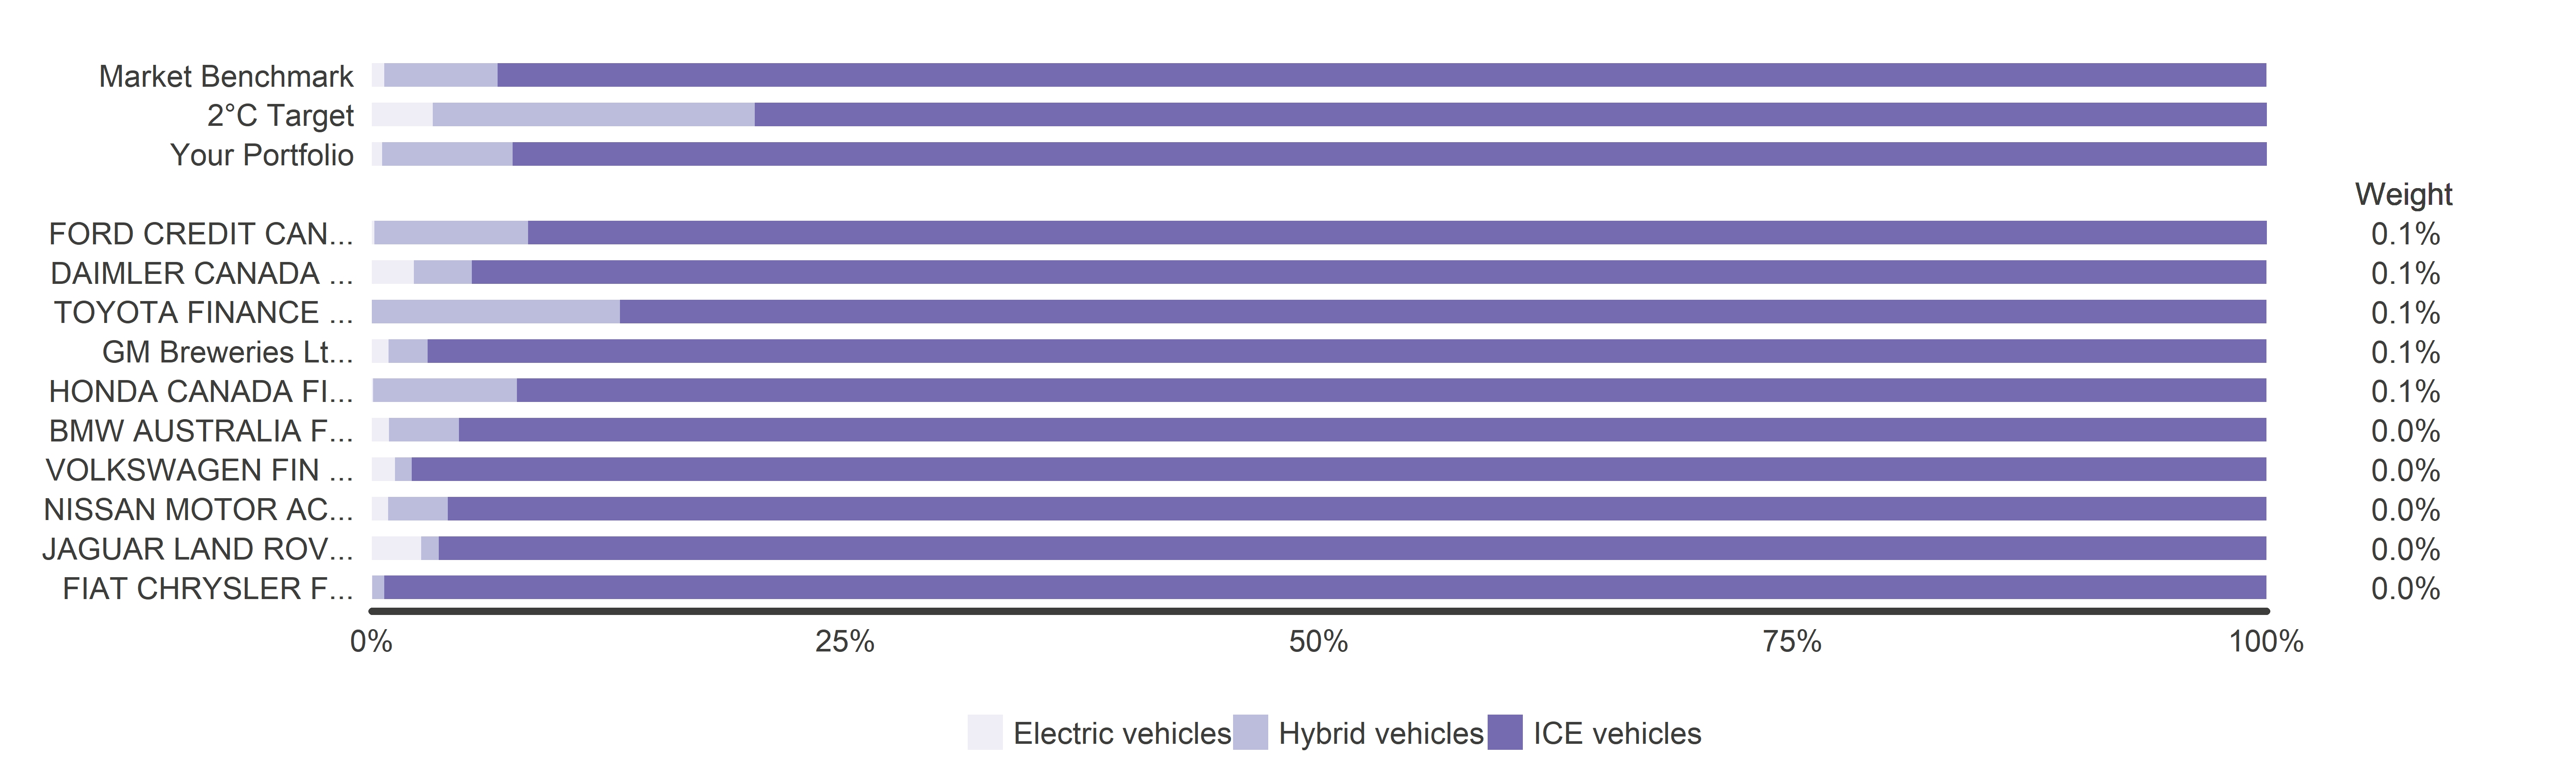
\includegraphics[trim = {0 0cm 0 0},width=1\linewidth]{Figures/Fig34}
			\end{center}
			%AutoSector_CBE
			%AutoSector_EQS
			\textbf{Technology breakdown of automotive companies within your equity portfolio}

			\begin{center}
			
				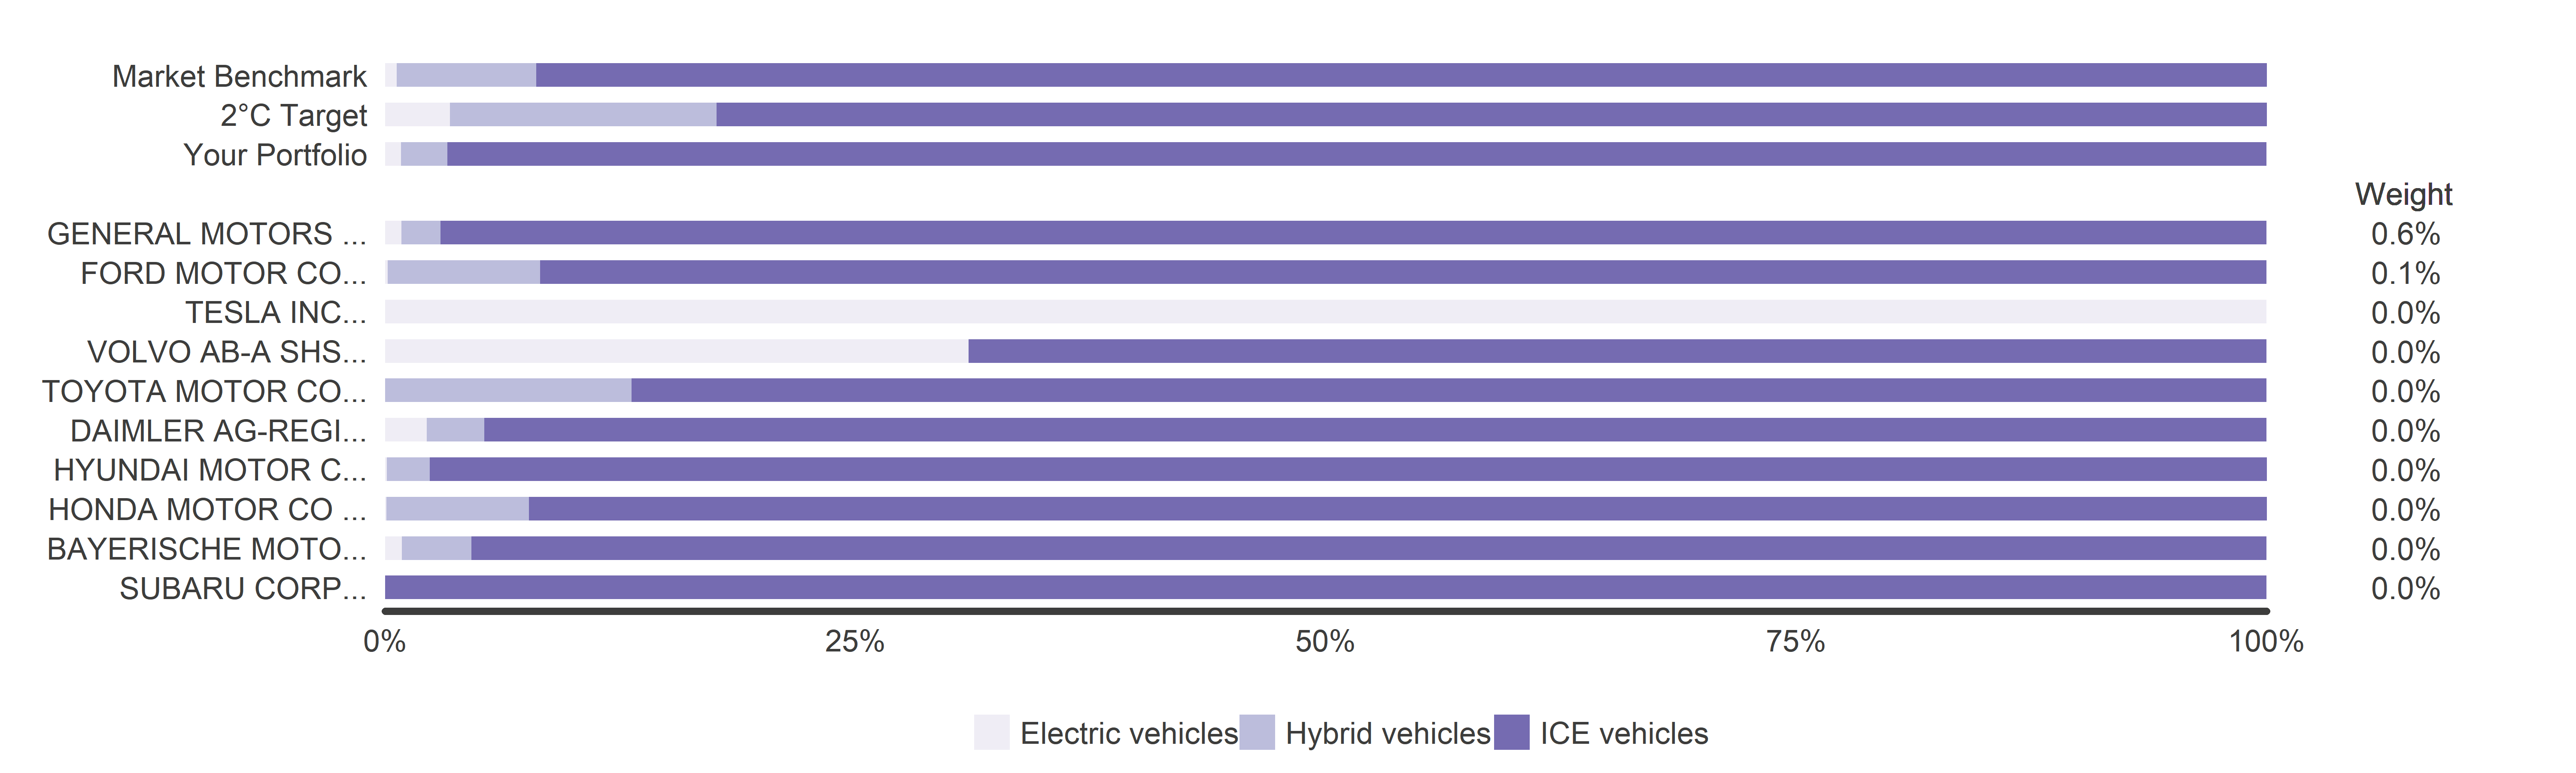
\includegraphics[trim = {0 0cm 0 0},width=1\linewidth]{Figures/Fig35}
			\end{center}
			%AutoSector_EQE
	
	\PageFooterFifth
	\newpage  
	%AutoSectorE  
\section*{} % 6th BACKGROUND
\SectionHeading{SECTION 5:}{BACKGROUND}


	\newpage	
	\section*{} %BACKGROUND TO THE MODEL
	\HeaderSingle{BACKGROUND TO THE MODEL}
	
		\begin{multicols}{2}
			\textbf{The objective of the assessment framework applied in this scenario analysis is to measure the alignment of financial portfolios with 2°C decarbonisation pathways. The model consists of 3 key elements that are detailed in the following pages.}
			
			
			\begin{itemize}
				
				\item {Scenarios, notably 2°C scenarios, that form the basis of the analysis and define the benchmark against which portfolio trends are compared. While in theory a range of scenarios can be applied for the model, in the interest of simplification, this analysis will rely on the scenarios of the International Energy Agency. These provide targets for each technology at a regional level. }
				
				\item{Financial portfolios and associated financial data to allow for the portfolio assessment. Within this report, the analysis will be limited to bonds and equity portfolio. Funds within your portfolio have been identified and the underlying financial data extracted from Morningstar and included as part of your portfolio. }
				
				\item{Physical / industry ‘asset level data’ (current and forward looking) is mapped to companies, parents, and securities. This allows the link between financial portfolios  and industry and production data (oil and gas production, automotive production, utilities) to be established. Consequently, this allows a comparison to the 2°C scenarios and a corresponding evaluation of the alignment of the portfolio. }
				
			\end{itemize}
		\end{multicols}
	
		
		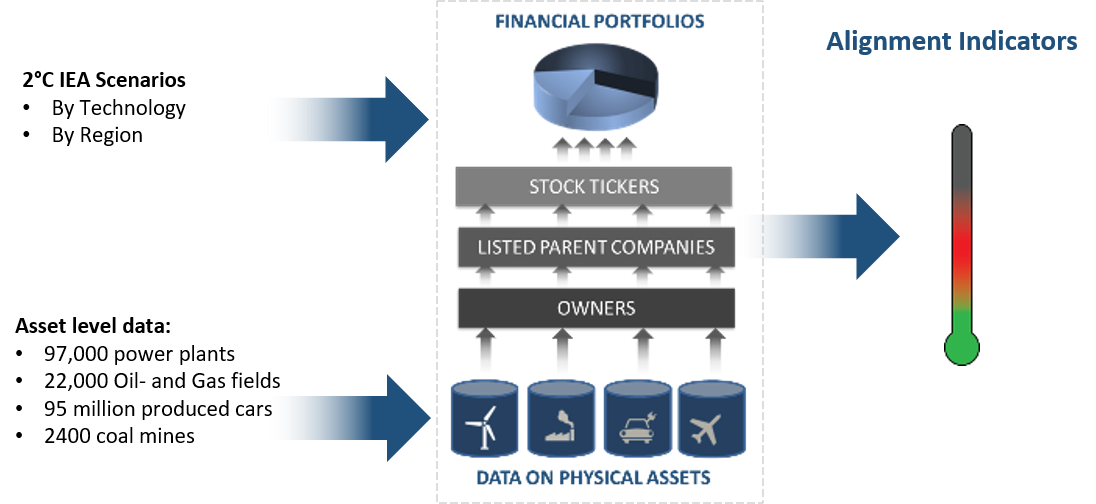
\includegraphics[trim = {0 0cm 0 0},width=1\linewidth]{ReportGraphics/SummaryChart}
		
		\begin{multicols}{2}
			\textbf{Allocation Rules}
			Based on the financial data, the asset level data is allocated to your portfolio to quantify a representative value of what your portfolio physically owns.  This allocation rules varies between equity and bond portfolios. For equity portfolios, the analysis is based on the ownership percentage of companies and their subsidiaries, with respect to all outstanding shares of the companies. This approach reflects the fact that the shares represent ownership ratios. In the case of bonds, exposure is determined based on the share in the portfolio of the relevant credit instrument. The underlying company exposure is defined by the technology mix (for example, the ratio of renewable to coal power). 
			
			\textbf{Benchmarking}
			Using the allocated production or capacity of technologies within your portfolio in as a starting point, an allowance based on the regional scenarios is calculated. This is extrapolated over the next 5 years to create the trajectory and this is compared to your current and future ownership. The variation of your ownership from this benchmark is used as the alignment indicator in the preceding results.  
		\end{multicols}



	\newpage	
	\section*{} %BACKGROUND TO THE MODEL
	\HeaderSingle{BACKGROUND TO THE MODEL}

		\begin{multicols}{2}
					\textbf{Scenarios}
			
			As outlined above, the underlying principle of the model is to compare the portfolio trends with a 2°C scenario. The model for this pilot relies on the International Energy Agency 2°C scenarios (labelled the 450 or 2D Scenario). A common, internationally recognized scenario framework was chosen to ensure comparability across results. The choice of the scenario should not be interpreted however as an endorsement of the underlying assumptions within the model and does not constitute an implicit or explicit assumption around the alignment with long-term climate policy positions. 
			
			The IEA historically has assumed significant amounts of nuclear power and carbon capture and storage in their scenarios. In addition, the international community has accelerated their global target from the 2°C goal to well below 2°C with a target of 1.5°C. It is important to highlight that each investor can and may want to take an individual view on the likely decarbonization scenario that may or may not relate to the scenarios modelled by the International Energy Agency or others.
			
			The model uses the following indicators from the International Energy Agency scenario against which the portfolio is compared:
			\begin{itemize}
				\item{Electric capacity by fuel expressed in MW (e.g. renewables, coal, gas, oil, hydropower, nuclear);}
				\item{Oil production expressed in barrels of oil produced / year;}
				\item{Gas production expressed in bcf / year;}
				\item{Coal produced expressed in mtoe / year;}
				\item{GHG emissions pathways in a sample of additional sectors (e.g. aviation, shipping, cement, steel).}
			\end{itemize}
			
			
			\textbf{Asset Level Data}
			
			The Asset Level data is sourced from the following data providers: 
			\begin{itemize}
				\item{GlobalData (Power plant data, including plants classified as active, announced, financed, partially active, permitting, temporarily shutdown, under construction, under rehabilitation and modernization, and Oil and Gas production data and forecast until 2018-2023, as well as coal mining data); }
				\item{WardsAuto (light passenger duty vehicle, including BAU production forecasts 2018-2023); }
				\item{Bloomberg (financial data);}
				\item{Orbis (database on matching company subsidiary trees);}
				\item{S\&P Cross-Reference Services (database matching securities to parents);}
				\item{Morningstar (database on funds). }
				
			\end{itemize}
			
			\textbf{Caveats / Notes on interpreting the results}
			
			The following briefly highlights key caveats to the model and the results:
			
			\begin{itemize}
				\item{The forward-looking data is based on current ‘revealed’ plans from companies and is subject to change. The estimates should thus not be interpreted as final forecasts, but rather the current plans of companies if they don’t change. Another way to interpret the results is the call for action with regard to the required change to align with the 2°C economic trend. Given the 5 year time horizon, there is a high degree of certainty that plans will still change in some way over time. Similarly, the participating financial institutions can of course alter their portfolio exposures over time. The analysis however seeks to be a point in time assessment of future exposures under current conditions.}
				\item{The model takes a diversified ‘market portfolio’ as a basis, focusing on key technologies reflected in the IEA roadmaps. By extension, thematic portfolios invested in breakthrough technologies and / or SRI portfolios with a range of environmental, social, and governmental considerations may not value these elements.}
			\end{itemize}
		\end{multicols}


	\newpage	
	\section*{} %INTERPRETATION AND IMPLICATIONS FOR RISK
	\HeaderSingle{INTERPRETATION AND IMPLICATIONS FOR RISK}
		
		\begin{multicols}{2}
				Important in the implementation of different actions based on the 2°C scenario analysis is an understanding of the implications for risk and return of the portfolio. It is important to emphasize here that the results presented in this report are explicitly not a risk analysis. In general, the following findings can be summarized as the interaction between risk, return, and the 2°C scenario analysis. 
			
			\textbf{What is the risk of inaction?}
			Although the analysis focuses on alignment with the Paris Agreement in a way that contributes to the general interest, the issue can also be addressed in terms of the financial risk to the investor if the energy transition is not properly anticipated. 
			
			For investors, the main risk seems to be more pronounced if the 2°C target is not reached. Aviva and the Economist Intelligence Unit analyzed the net impairment loss for financial assets under management at approximately USD60 trillion in a 2°C scenario (Aviva 2015). The TCFD (Task Force on Climate-related Financial Disclosures) initiated by the Financial Stability Committee (FSB) calls these risks ”physical risks”. If the 2°C objective is achieved, these physical risks can be reduced considerably. The cost would be limited to less than USD10 trillion if we remain below 3°C according to the same Aviva / ECIU estimates. 
			
			However, investment portfolios can then be exposed to what the TCFD calls ”transition risks” - the economic and financial risks associated with the transition to a low-carbon economy. These risks are likely to be particularly pronounced for the most CO\textsubscript{2}-emitting sectors, and thus their investors. Most of these sectors are covered by our analysis in the previous sections. 
			
			Although the 2°C scenario presented in this report is not directly a financial risk assessment, it can help to better understand the exposure to transition risk faced by investors. It makes it possible to understand whether the necessary transition will be gradual (when the production and investment plans are aligned with the 2°C scenario) or is likely to be abrupt (sudden correction linked to the introduction of new technologies or constraints legal proceedings leading to bankruptcies of established companies). All investment strategies are exposed to potential risks. The scenario analysis reveals how each strategy evaluated is an explicit or implicit bet on a 2°C, 4°C or 6°C scenario. Depending on the trajectory that will ultimately prevail, the portfolios will underperform or outperform. From the point of view of the optimization of the risk/return ratio in the long term, it is essential to be aware of the bet made.
			
			From a transition risk perspective, the following three questions are important:
			
			\begin{enumerate}
				\item{Is my portfolio over-exposed to transition risks by deviating from the 2°C benchmark?}
				\item{If this is the case, which securities in my portfolio are exposed to these risks?}
				\item{Should these risks arise, what are possible losses?}
			\end{enumerate}
			
			
			The answer to the first question is provided by the analysis presented in the previous pages. There are different approaches to quantifying exposure:
			
			\begin{itemize}
				\item{Based on the method presented in this report, it is possible to isolate the most misaligned sectors and securities with respect to a 2°C trajectory.}
				
				\item{The rating agency Moody’s developed in 2016 a methodology to classify the different sectors of their bond universe according to the risk of downgrade due to environmental risk.}
			\end{itemize}
			
			
			\textbf{Asset Pricing and Risk} 
			A final question to be considered is: what is the potential value at risk within the climate relevant sectors if a 2° C scenario materializes? This requires additional financial analysis. In particular, assumptions must be made as to how the market has already (or not) integrated these risks into the current price of financial assets. There are several research papers on the subject, published by financial analysts, NGOs and consultants, covering equities and credit (2ii 2018). 
			
			In all this, it is important to emphasize that asset prices - based on market participants’ assumptions about changes in the yield-risk profile of securities - do not necessarily reflect the economic risks faced by a company. Thus, the price of assets , and the risk that their valuation will decrease, does not automatically reflect the underlying risks to which the companies are exposed. On the other hand, it should be noted that the return potential is optimized when the allocation of capital is as efficient as possible. If the capital is not allocated efficiently, the absolute benefit is also reduced. Signals issued by the financial markets in the form of portfolio reallocation choices or via shareholder engagement can thus help optimize the allocation of capital in the real economy, and help maximize long-term returns.
		\end{multicols}
	
		
		\newpage	
	\section*{} %NOTES AND DISCLAIMER
	\HeaderSingle{NOTES AND DISCLAIMER}
	
		\begin{multicols}{2}
				The data and scenario sources for this analysis are shown below. 
			
			\textbf{Published Research}
			
			The methodology behind this scenario analysis, the accounting rules applied, and further information to the scenarios and data can be found in the following published research papers. 
			
			Accounting Principles: http://www.mdpi.com/2071-1050/ 10/2/328 
			
			Scenario Work: http://et-risk.eu/toolbox/ scenarios/ 
			
			Asset Level Data Analysis: http://2degrees-investing.org/ IMG/pdf/assetdata\_v0.pdf
			
			\textbf{Sources for the data and scenario analysis}
			
			Automobile data are from July 2018 and is provided by WardsAuto / AutoForecastSolutions. Power data is from July 2018 and is provided by GlobalData. Oil, gas and coal production data is from July 2018 and is provided by GlobalData. When linking asset data with companies, the data is used by the data providers mentioned above and, where possible, enriched with company data from Bloomberg. All financial data, as well as identification numbers for linking company data with financial instruments, come from Bloomberg. The decarbonization pathways for other sectors comes from the Science-Based Targets Initiative, which bases its methodology on the IEA scenarios. The scenarios for the energy and power sector come from the IEA’s World Energy Outlook 2016. Because this report does not include scenario information for the automotive sector, the related data is taken from the sister report of the World Energy Outlook, the Energy Technology Perspective report. Benchmarks for the electricity sector are determined regionally and applied in relation to the regional exposure data and then aggregated, weighted according to the regional exposure of the portfolio. All other results are global.
			
			\textbf{Sources}
			
			IPCC (2018) https://www.ipcc.ch/report/ar5/
			
			FSB (2018) https://www.fsb-tcfd.org/publications/final-recommendations-report/
			
			Aviva / ECIU (2015) https://www.aviva.com/media/thought-leadership/climate-change-value-risk-investment-and-avivas-strategicresponse/
			
			FSB (2018) https://www.fsb-tcfd.org/publications/final-recommendations-report/
			
			WoodMackenzie (2018) https://www.woodmac.com/news/ editorial/carbon-intensity-not-all-assets-are-created-equal/ 
			
			\textbf{Disclaimer}
			
			The 2° Investing Initiative’s research is provided free of charge and 2°ii does not seek any direct or indirect financial compensation for its research. 2°ii is not an investment adviser and makes no representation regarding the advisability of investing in any particular company or investment fund or other vehicle. A decision to invest in any such investment fund or other entity should not be made in reliance on any of the statements set forth on this website and the analysis results. The information and analysis contained in this research report does not constitute an offer to sell securities or the solicitation of an offer to buy, or recommendation for investment, in any securities within the United States or any other jurisdiction. The information is not intended as financial advice. The research report and website results provide general information only. The information and opinions constitute a judgment as at the date indicated and are subject to change without notice. No representation or warranty, express or implied, is made by 2°ii as to their accuracy, completeness or correctness. 2°ii does not warrant that the information is up to date, nor does it take liability for errors in third-party sourced data.
		\end{multicols}

	


\end{document} 
